\documentclass[preprint,12pt]{elsarticle}

% Encoding and fonts
\usepackage[T1]{fontenc}
\usepackage[utf8]{inputenc}
\usepackage{lmodern}

% Math packages
\usepackage{amsmath}
\usepackage{amssymb}
\usepackage{amsfonts}
\usepackage{amsthm}
\usepackage{mathtools}

% Layout and utilities
\usepackage{enumitem}
\usepackage{booktabs}
\usepackage{graphicx}
\usepackage{xcolor}
\usepackage[hidelinks]{hyperref}
\makeatletter
\pdfstringdefDisableCommands{%
  \def\corref#1{}%
  \def\cnotenum{}%
  \def\@corref{}%
}
\makeatother

\numberwithin{equation}{section}
\emergencystretch=3em
\setcounter{tocdepth}{3}
\setcounter{secnumdepth}{3}

% ---------------------------------------------------------
% Theorem-like environments
% ---------------------------------------------------------
\theoremstyle{plain}
\newtheorem{theorem}{Theorem}[section]
\newtheorem{proposition}[theorem]{Proposition}
\newtheorem{lemma}[theorem]{Lemma}
\newtheorem{corollary}[theorem]{Corollary}
\newtheorem{conjecture}[theorem]{Conjecture}

\theoremstyle{definition}
\newtheorem{definition}[theorem]{Definition}
\newtheorem{experiment}[theorem]{Experiment}
\newtheorem{heuristic}[theorem]{Heuristic}

\theoremstyle{remark}
\newtheorem{remark}[theorem]{Remark}
\newtheorem{warning}[theorem]{Warning}

\newcommand{\RH}{\mathrm{RH}}
\newcommand{\Li}{\lambda}
\newcommand{\E}{\mathsf E}
\newcommand{\Omat}{\mathsf O}
\newcommand{\Kmat}{\mathsf K}
\newcommand{\J}{\mathsf J}
\newcommand{\e}{\mathrm e}
\newcommand{\dd}{\,\mathrm d}
\newcommand{\diag}{\operatorname{diag}}
\newcommand{\rank}{\operatorname{rank}}
\newcommand{\spec}{\operatorname{spec}}
\newcommand{\Span}{\operatorname{span}}
\newcommand{\Tr}{\operatorname{Tr}}
\journal{Linear Algebra and its Applications}

\begin{document}
\begin{frontmatter}
\title{Reflection Li--Weil Matrices:\\Determinant Geometry, Local Pivot Dynamics, and Jacobi Spectral Encoding}
\author[uned]{Víctor Casaña-Giner\corref{cor1}}
\ead{vcasana1@alumno.uned.es}
\cortext[cor1]{Corresponding author}
\affiliation[uned]{organization={Universidad Nacional de Educación a Distancia},
                  city={Madrid},
                  country={Spain}}

\begin{abstract}
We study two even/odd reflection compressions of the bilateral Li--Weil kernel, separating
results independent of the Riemann Hypothesis (\(\RH\)) from those that assume it.  Unconditionally,
we establish the Toeplitz--Hankel reflection form, exact reconstruction of the Li sequence,
reflected Weil-pairing identities, discrete wave equations, rank-two displacement, closed
bordering recursions, and a local \(LDL^T\) pivot law; the even family alone also yields a matrix
criterion equivalent to \(\RH\).  Under \(\RH\), the matrices become positive sine Gram systems on
the Cayley images of the zeta zeros.  This gives positive Chebyshev moment measures, exact
Cauchy--Binet--Vandermonde expansions, a fixed-size projection determinantal process, and infinite
Jacobi operators whose spectral supports and scaled cyclic measures recover distinct ordinates and
multiplicities.  We also obtain the critical Schatten exponent \(1/2\) and exact
Christoffel/Darboux and Fredholm determinant relations.  Independently of \(\RH\), an endpoint
theorem proves \(\log D_N=-\beta N^2\log N+o(N^2\log N)\) under explicit node-scale, separation,
and weight hypotheses; \(\beta\) alone is insufficient.  For the Li--Cayley measures these
hypotheses give coefficient \(-2\) under \(\RH\).  A second-order \(N^2\log\log N\) law requires
additional gap and weight assumptions and is not deduced from \(\RH\).  Finally, the independent
unconditional zeta-value Hankel family satisfies
\(\log\det(\zeta(a(i+j)+b))_{1\le i,j\le n}=-a n^2\log n+O(n^2)\).
\end{abstract}

\begin{keyword}
Li coefficients \sep Riemann Hypothesis \sep Weil criterion \sep Toeplitz--Hankel matrices
\sep Hankel determinants \sep Jacobi operators

\MSC[2020] 15B05 \sep 15A15 \sep 47B36 \sep 11M26 \sep 11C20
\end{keyword}
\end{frontmatter}

\section{Introduction}
The aim of this paper is to isolate, with complete proofs, the exact
mathematical consequences of a pair of reflection compressions of the bilateral Li--Weil kernel.
The scalar Li criterion and the bilateral Weil kernel are classical.  The objects developed here
are the even and odd reflection arrays and the finite- and infinite-dimensional structures
generated by them.

The logical status of every result is separated explicitly.  Reflection definitions,
reconstruction formulas, wave and displacement identities, bordering recursions, and local
elimination identities are unconditional.  Positive zero-side Gram, moment, determinantal-process,
and Jacobi descriptions assume \(\RH\).  The abstract endpoint theorem is independent of
\(\RH\), but it requires explicit geometric hypotheses on node scale, separation, and weights.
Its Li--Cayley specialization uses \(\RH\) to obtain a positive moment representation, whereas
the final zeta-value Hankel application is unconditional.

The matrix-theoretic viewpoint also places the present work within several themes developed in
\emph{Linear Algebra and its Applications}.  The direct link between semi-infinite Hankel and
Jacobi matrices through commutation and orthogonal-polynomial structures was investigated by
\v{S}tampach and \v{S}\v{t}ov\'i\v{c}ek~\cite{StampachStovicek2020}; our construction uses a
different mechanism, namely the moment matrix of a positive measure and its three-term Jacobi
recurrence.  Structured rank deficiency and low-rank approximation for Hankel matrices were
studied by Fazzi, Guglielmi and Markovsky~\cite{FazziGuglielmiMarkovsky2021}, while fixed-rank
matrix perturbations and their determinant constraints were treated by Baraga\~na and
Roca~\cite{BaraganaRoca2020}.  At the level of determinantal algebra, compound-matrix and
Binet--Cauchy-type identities also form an active line of research in the journal, including the
tropical framework of Akian, Gaubert and Niv~\cite{AkianGaubertNiv2018}.  These works address
different problems, but they provide a natural linear-algebraic context for the Hankel, Jacobi,
low-rank displacement, compound-minor and determinant structures developed below.

\subsection{Main contributions}
\label{subsec:main_contributions}
The main contributions are the following.
\begin{enumerate}[label=\textup{(\arabic*)},leftmargin=2.5em]
\item We introduce the even and odd reflection arrays
\[
e_{mn}=\lambda_{m+n}-\lambda_{|m-n|},
\qquad
o_{mn}=\lambda_{m+n-1}-\lambda_{|m-n|},
\]
and determine their unconditional information content.  The odd semi-infinite first row
reconstructs the complete Li sequence; the odd reflection map is injective; and the kernel of
the even reflection map is identified exactly.
\item We prove unconditional reflected Weil-pairing formulas, discrete wave equations,
rank-two displacement identities, inverse-displacement identities whenever the relevant blocks
are invertible, closed bordering recursions, and a local \(LDL^T\) pivot dynamics controlled by
the first two elimination subdiagonals.
\item We obtain matrix criteria equivalent to \(\RH\).  Positivity of all even and odd leading
reflection blocks is equivalent to the Li criterion, and the even family alone is shown to be
sufficient through a transformed Bombieri--Lagarias multiset.
\item Assuming \(\RH\), we construct the positive sine Gram and Chebyshev moment realizations.
They lead to exact Cauchy--Binet--Vandermonde formulas, a fixed-order projection determinantal
ensemble, zero deletion and transport identities, and high-zero leverage estimates whose scope
is explicitly restricted to fixed matrix order.
\item We prove an abstract endpoint-exponent theorem for positive discrete Gram determinants.
Its conclusion is not a consequence of \(\beta\) alone: the theorem identifies the precise
node-scale, separation, and weight assumptions under which the leading coefficient is
\(-\beta\).  Applying it to the Li--Cayley support gives coefficient \(-2\) under \(\RH\).
\item Under \(\RH\), we construct infinite Jacobi operators with exact spectral support,
distinguish support recovery from multiplicity recovery, determine the critical Schatten
exponent, and derive the Christoffel/Darboux and Fredholm determinant relations between the
even and odd systems.
\item We isolate a second-order law under hypotheses strictly stronger than \(\RH\), and we give
an independent unconditional application to Hankel determinants of zeta values with leading
term \(-a n^2\log n\).
\end{enumerate}

\medskip
\noindent\textbf{Novelty boundary.}
No novelty is claimed for the scalar Li criterion, the Bombieri--Lagarias multiset criterion,
the bilateral Weil kernel, standard moment-matrix or Jacobi theory, or the generic occurrence of
\(N^2\log N\) scales in discrete determinants.  The contribution developed here is the specific
even/odd reflection package, its exact Toeplitz--Hankel, wave, displacement, elimination,
determinantal, and spectral structures, and the endpoint analysis of the Li--Cayley measures.
All priority claims are limited to the precise statements proved in this paper.

For orientation, other zeta-associated matrix programs include Roesler's eigenvalue
formulations \cite{Roesler1986,Roesler1987}, spectral analysis of Redheffer matrices
\cite{Vaughan1996}, and multiplicative Toeplitz matrices tied to the zeta function
\cite{Hilberdink2006,Hilberdink2015}. Those constructions are structurally distinct from
the reflection matrices studied here; they are mentioned to position the present matrix
framework within the broader linear-algebraic literature surrounding the zeta function.

\subsection{Guide to hypotheses and proofs}
\label{subsec:proof_audit_guide}
The proof architecture can be audited in the following order.
\begin{enumerate}[label=\textup{(\alph*)},leftmargin=2.5em]
\item The algebraic reflection results use only the Li sequence and explicitly stated
nonsingularity assumptions when an inverse or pivot is formed.
\item The even-only equivalence uses the Bombieri--Lagarias criterion, but does not assume
\(\RH\).
\item The sine Gram, positive moment, determinantal-process, and Jacobi layers begin only after
\(\RH\) is assumed.
\item The abstract endpoint theorem uses its four displayed hypotheses.  In the Li--Cayley
application, standard zero counting verifies the first-order node and separation requirements;
no unproved gap hypothesis is used for the coefficient \(-2\).
\item The second-order refinement adds explicit scale, aggregate-gap, and weight hypotheses and
is not deduced from \(\RH\).
\item The zeta-value Hankel application uses a separate positive Dirichlet-series measure and
does not use \(\RH\) or the zeta-zero measures.
\end{enumerate}
Subsection~\ref{subsec:logical_status} gives the complete hypothesis table, and
Figure~\ref{fig:structural_map} displays the same dependency structure graphically.

For later reference, Lagarias's bilateral Li test functions are
\begin{equation}
G_k(s):=1-\left(1-\frac1s\right)^k,
\qquad k\in\mathbb Z,
\label{eq:intro_Lagarias_test}
\end{equation}
and their Weil Gram kernel is
\begin{equation}
\langle G_r,G_s\rangle_W
=\lambda_r+\lambda_s-\lambda_{|r-s|}.
\label{eq:intro_Lagarias_Gram}
\end{equation}
The reflected test vectors used throughout are
\begin{equation}
F_n^E=\frac{G_n-G_{-n}}{\sqrt2},
\qquad
F_n^O=\frac{G_n-G_{1-n}}{\sqrt2}.
\label{eq:intro_reflected_tests}
\end{equation}

\section{Definitions and conventions}
\label{sec:notation_definitions}

The following conventions are used throughout.

\begin{description}[style=nextline,leftmargin=2.2em,itemsep=5pt]
\item[Zeros and multiplicity]
A nontrivial zero of \(\zeta\) is denoted by \(\rho\).  Under \(\RH\) we write
\(\rho=\tfrac12+i\gamma\) with \(\gamma>0\).  The symbol \(m_\gamma\) denotes the
multiplicity of the ordinate \(\gamma\).  Sums over \(\gamma>0\) count multiplicity unless
the set \(\Gamma_+^*\) of distinct positive ordinates is displayed explicitly.

\item[Li coefficients]
The coefficients \(\lambda_n\) are defined by \eqref{eq:li_derivative_definition} below,
with \(\lambda_0=0\).  For the bilateral Li--Weil kernel we use the even extension
\(\lambda_{-n}=\lambda_n\).

\item[Reflection matrices]
For \(m,n\ge1\),
\[
e_{mn}:=\lambda_{m+n}-\lambda_{|m-n|},
\qquad
o_{mn}:=\lambda_{m+n-1}-\lambda_{|m-n|},
\]
and \(\E_N=(e_{mn})_{m,n\le N}\), \(\Omat_N=(o_{mn})_{m,n\le N}\).
Their leading determinants are
\[
\Delta_N^E:=\det\E_N,\qquad
\Delta_N^O:=\det\Omat_N,\qquad
\Delta_0^E=\Delta_0^O:=1.
\]
Whenever the preceding leading block is nonsingular, the corresponding Schur or
\(LDL^T\) pivot is
\[
p_N^E:=\frac{\Delta_N^E}{\Delta_{N-1}^E},
\qquad
p_N^O:=\frac{\Delta_N^O}{\Delta_{N-1}^O}.
\]

\item[Li--Cayley coordinates]
For a zero \(\rho\) put \(q_\rho:=1-\rho^{-1}\).  Under \(\RH\),
\(q_\rho=e^{i\theta_\gamma}\) and
\[
x_\gamma:=\cos\theta_\gamma
=\frac{4\gamma^2-1}{4\gamma^2+1},
\qquad
1-x_\gamma=\frac{2}{4\gamma^2+1}.
\]
Thus \(x_\gamma\uparrow1\) as \(\gamma\to\infty\).

\item[Moment determinants]
For a finite positive discrete measure
\(\mu=\sum_jw_j\delta_{x_j}\), its monomial Gram or Hankel determinant is
\[
D_N[\mu]
:=\det\left(\int x^{r+s}\,\dd\mu(x)\right)_{r,s=0}^{N-1}.
\]
The endpoint exponent \(\beta\) refers only to the local support law
\(1-x(t)\asymp t^{-\beta}\), or its regularly varying form.  By itself this exponent does
\emph{not} determine the determinant asymptotic; the endpoint theorem also imposes separate
hypotheses on the node scale, a separated subconfiguration, and the selected weights.

\item[Jacobi operators]
For either normalized reflection measure, \(\mathcal J\) denotes the Jacobi operator
unitarily equivalent to multiplication by \(x\).  Its defect is
\(\mathcal D:=I-\mathcal J\).  The Schatten ideal of order \(p>0\) is denoted by
\(\mathcal S_p\).

\item[Zero-index kernels]
At fixed matrix order \(N\), the zero-side Gram factorization is \(M_N=AA^T\) and
\[
K_N:=A^TM_N^{-1}A.
\]
A repeated zero is represented by repeated identical columns, one for each multiplicity
index.

\item[Asymptotic notation]
All \(O(\cdot)\), \(o(\cdot)\), \(\ll\), and \(\asymp\) statements are taken in the
indicated asymptotic variable; constants may depend on fixed matrix order or fixed
parameters when this is explicitly stated.
\end{description}

\subsection{Logical status of the main results}
\label{subsec:logical_status}
The phrases ``unconditional'', ``under \(\RH\)'', and ``under endpoint hypotheses'' are used in a
literal logical sense throughout the paper.  In particular, the abstract endpoint theorem is not a
consequence of \(\RH\), and the positive zero-side moment/Jacobi constructions are not asserted
without \(\RH\).  The main blocks are as follows.

\begin{center}
\small
\begin{tabular}{p{0.30\textwidth}p{0.19\textwidth}p{0.39\textwidth}}
\toprule
\textbf{Block} & \textbf{Logical status} & \textbf{Input beyond definitions}\\
\midrule
Reflection reconstruction, wave equation, displacement and local \(LDL^T\) identities
& Unconditional & Algebra of the Li sequence; nonsingularity only where an inverse or pivot is used.\\
Exact reflected Weil pairing
& Unconditional identity & Classical bilateral Li--Weil kernel.\\
Even-family matrix criterion
& Equivalence to \(\RH\) & Bombieri--Lagarias multiset criterion; no prior assumption of \(\RH\).\\
Sine Gram, positive moment measures, Cauchy--Binet zero ensemble
& Under \(\RH\) & Zeros written as \(1/2+i\gamma\), hence positive Cayley weights.\\
Jacobi zero spectrum, cyclic masses, Schatten and Christoffel/Darboux theory
& Under \(\RH\) & Positive reflection measures from the preceding row.\\
Endpoint-exponent theorem
& Unconditional theorem under hypotheses & Endpoint law plus node-density, separated-subconfiguration and weight hypotheses.\\
Li--Weil coefficient \(-2\)
& Under \(\RH\) & Positive Li--Cayley measures; the endpoint hypotheses are then verified from zero counting.\\
Second-order \(N^2\log\log N\) law
& \(\RH\) plus extra hypotheses & Strengthened node scale, gap regularity and weight asymptotics.\\
Zeta-value Hankel law \(-a n^2\log n+O(n^2)\)
& Unconditional & Positive Dirichlet-series moment measure with node scale \(t_j=j\).\\
\bottomrule
\end{tabular}
\end{center}

Figure~\ref{fig:structural_map} summarizes these dependencies.  Blue arrows in the figure are
unconditional, green arrows are implications made after assuming \(\RH\), orange dashed arrows
use the abstract endpoint hypotheses, and the red branch is the external unconditional zeta-value
Hankel application.

\begin{figure}[t]
\centering
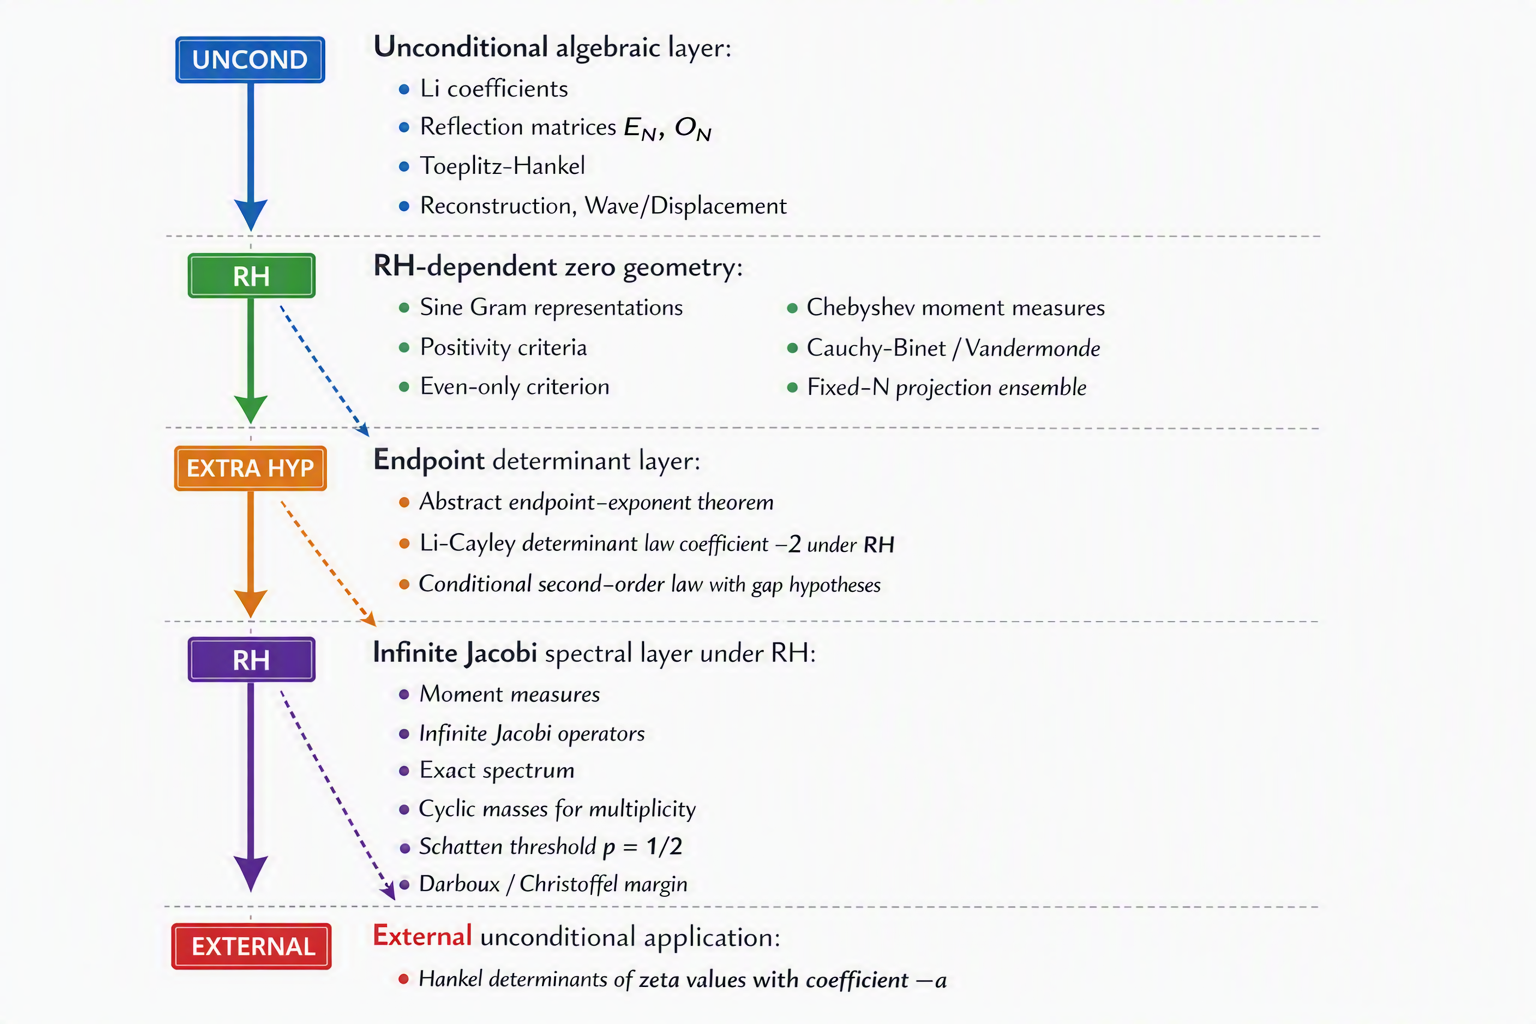
\includegraphics[width=\textwidth]{reflection_li_weil_dependency_map.png}
\caption{Dependency map with logical status made explicit.  Blue arrows are unconditional;
green arrows require \(\RH\); orange dashed arrows invoke the abstract endpoint hypotheses; the
red branch is the external unconditional zeta-value Hankel application.  The \(-2\) Li--Weil law
therefore belongs to the RH branch because the positive Li--Cayley moment measures do, whereas the
endpoint theorem itself does not assume \(\RH\).}
\label{fig:structural_map}
\end{figure}

\section{The xi-function and Li coefficients}
\label{sec:li_background}

Define the completed zeta-function
\begin{equation}
\xi(s)=\frac12 s(s-1)\pi^{-s/2}\Gamma\!\left(\frac{s}{2}\right)\zeta(s).
\label{eq:xi_definition}
\end{equation}
It is entire of order one and satisfies
\begin{equation}
\xi(s)=\xi(1-s)=\overline{\xi(\overline{s})}.
\label{eq:xi_symmetry}
\end{equation}
Riemann's original memoir introduced the analytic framework behind this completion
\cite{Riemann1859}; a modern overview of the hypothesis and its context is given by
Conrey~\cite{Conrey2003}.  The standard analytic theory may be found in
\cite{Edwards1974,Titchmarsh1986,Bombieri2010}.

\begin{definition}[Li coefficients]
\label{def:li_coefficients}
For $n\ge1$, define
\begin{equation}
\lambda_n=
\frac{1}{(n-1)!}
\left.
\frac{\dd^n}{\dd s^n}
\left[s^{n-1}\log\xi(s)\right]
\right|_{s=1},
\qquad \lambda_0:=0.
\label{eq:li_derivative_definition}
\end{equation}
Equivalently, with the symmetric limiting convention over nontrivial zeros,
\begin{equation}
\lambda_n=
\sum_{\rho}
\left[1-\left(1-\frac1\rho\right)^n\right].
\label{eq:li_zero_definition}
\end{equation}
\end{definition}

These numbers are also called the Keiper--Li coefficients: the power-series expansion of $\log\xi$
underlying \eqref{eq:li_derivative_definition} and its high-precision evaluation were studied by
Keiper~\cite{Keiper1992} before Li's positivity criterion appeared.  Subsequent formulations and
computational perspectives on these coefficients include
\cite{Coffey2007ThetaLaguerre,Coffey2010Polygamma,Coffey2010ZeroSums,
Matiyasevich2007a,Matiyasevich2007b}.

For the zeta xi-function the zero symmetry implies an integer-index extension
\begin{equation}
\lambda_{-n}=\lambda_n
\qquad(n\ge1),
\label{eq:li_negative_symmetry}
\end{equation}
as recorded, for example, in \cite[Eq.~(1.2)]{Lagarias2007}. This identity is unconditional and will be used whenever differences of integer indices occur.

\begin{theorem}[Li]
\label{thm:li_criterion}
The Riemann hypothesis is equivalent to
\begin{equation}
\lambda_n\ge0
\qquad\text{for every }n\ge1.
\label{eq:li_criterion}
\end{equation}
\end{theorem}

\begin{proof}
This is Li's positivity criterion \cite{Li1997}; see also \cite{BombieriLagarias1999,Lagarias2007}.
\end{proof}

Li-type criteria have also been developed for zero-free half-planes, extensions of the Selberg
class, Hecke and related \(L\)-functions, and generalized Bombieri--Lagarias settings; see
\cite{Freitas2006,Droll2012,OmarOuniMazhouda2014,OmarOuni2017,
Sekatskii2014,BucurErnvallOdzakSmajlovic2016,Palojarvi2018}.  None of those variants is used below.

Define
\begin{equation}
R_\xi:=\min\!\left\{1,\inf_{\rho}\left|1-\frac1\rho\right|\right\}.
\label{eq:li_generating_radius}
\end{equation}
The Li generating identity is the formal power-series identity
\begin{equation}
\Lambda(z):=\sum_{n\ge1}\lambda_n z^n
=
\frac{z}{(1-z)^2}
\frac{\xi'}{\xi}\!\left(\frac{1}{1-z}\right).
\label{eq:li_generating_function}
\end{equation}
Analytically, \eqref{eq:li_generating_function} holds in the disk $|z|<R_\xi$. Under $\RH$, every nontrivial zero satisfies $|1-1/\rho|=1$, and therefore $R_\xi=1$. If $\RH$ fails, a zero with real part $>1/2$ produces a singularity with $|1-1/\rho|<1$, so the unconditional radius must not be stated as $1$.

Under $\RH$ we may parameterize each zero in the upper half-plane by
\begin{equation}
\rho=\frac12+i\gamma,
\qquad
1-\frac1\rho=\e^{i\theta_\gamma},
\qquad 0<\theta_\gamma<\pi.
\label{eq:theta_parameterization}
\end{equation}
A direct calculation gives
\begin{align}
\cos\theta_\gamma
&=\frac{4\gamma^2-1}{4\gamma^2+1},
\label{eq:theta_cos}\\
\sin\theta_\gamma
&=\frac{4\gamma}{4\gamma^2+1}.
\label{eq:theta_sin}
\end{align}
Pairing conjugate zeros in \eqref{eq:li_zero_definition} yields the absolutely convergent representation
\begin{equation}
\lambda_n
=2\sum_{\gamma>0}
\left(1-\cos(n\theta_\gamma)\right).
\label{eq:li_cosine_representation}
\end{equation}
For fixed $n$, the summands are $O_n(\gamma^{-2})$.

\section{Definition of the reflection matrices}
\label{sec:definitions}

\begin{definition}[Even and odd reflection matrices]
\label{def:reflection_matrices}
For $N\ge1$, define
\begin{align}
\E_N
&:=\left(e_{mn}\right)_{m,n=1}^N,
&
e_{mn}&:=\lambda_{m+n}-\lambda_{|m-n|},
\label{eq:E_definition}\\
\Omat_N
&:=\left(o_{mn}\right)_{m,n=1}^N,
&
o_{mn}&:=\lambda_{m+n-1}-\lambda_{|m-n|}.
\label{eq:O_definition}
\end{align}
\end{definition}

Both are real symmetric. Their first $4\times4$ truncations are
\begin{equation}
\E_4=
\begin{pmatrix}
\lambda_2&\lambda_3-\lambda_1&\lambda_4-\lambda_2&\lambda_5-\lambda_3\\
\lambda_3-\lambda_1&\lambda_4&\lambda_5-\lambda_1&\lambda_6-\lambda_2\\
\lambda_4-\lambda_2&\lambda_5-\lambda_1&\lambda_6&\lambda_7-\lambda_1\\
\lambda_5-\lambda_3&\lambda_6-\lambda_2&\lambda_7-\lambda_1&\lambda_8
\end{pmatrix},
\label{eq:E4}
\end{equation}
and
\begin{equation}
\Omat_4=
\begin{pmatrix}
\lambda_1&\lambda_2-\lambda_1&\lambda_3-\lambda_2&\lambda_4-\lambda_3\\
\lambda_2-\lambda_1&\lambda_3&\lambda_4-\lambda_1&\lambda_5-\lambda_2\\
\lambda_3-\lambda_2&\lambda_4-\lambda_1&\lambda_5&\lambda_6-\lambda_1\\
\lambda_4-\lambda_3&\lambda_5-\lambda_2&\lambda_6-\lambda_1&\lambda_7
\end{pmatrix}.
\label{eq:O4}
\end{equation}

\begin{proposition}[Toeplitz--Hankel decomposition]
\label{prop:toeplitz_hankel}
Let
\begin{equation}
\mathsf T_N:=\bigl(\lambda_{|m-n|}\bigr)_{m,n=1}^N,
\label{eq:T_definition}
\end{equation}
\begin{equation}
\mathsf H_N^{(0)}:=\bigl(\lambda_{m+n}\bigr)_{m,n=1}^N,
\qquad
\mathsf H_N^{(-1)}:=\bigl(\lambda_{m+n-1}\bigr)_{m,n=1}^N.
\label{eq:H_definitions}
\end{equation}
Then
\begin{equation}
\E_N=\mathsf H_N^{(0)}-\mathsf T_N,
\qquad
\Omat_N=\mathsf H_N^{(-1)}-\mathsf T_N.
\label{eq:toeplitz_hankel_decomposition}
\end{equation}
Moreover,
\begin{equation}
\E_N-\Omat_N
=\bigl(\lambda_{m+n}-\lambda_{m+n-1}\bigr)_{m,n=1}^N,
\label{eq:E_minus_O}
\end{equation}
which is a pure Hankel matrix.
\end{proposition}

\begin{proof}
All statements follow directly from \eqref{eq:E_definition} and \eqref{eq:O_definition}.
\end{proof}

\section{Algebraic reconstruction and information content}
\label{sec:algebraic_reconstruction}

The two arrays contain substantial algebraic redundancy.  This can be described exactly without assuming $\RH$.

\begin{proposition}[Reconstruction from the infinite first rows]
\label{prop:first_row_reconstruction}
Since
\begin{equation}
o_{1j}=\lambda_j-\lambda_{j-1},
\qquad j\ge1,
\label{eq:odd_first_row_differences}
\end{equation}
one has
\begin{equation}
\lambda_n=\sum_{j=1}^{n}o_{1j}
\qquad(n\ge1),
\label{eq:lambda_from_O_first_row}
\end{equation}
and, for all $m,n\ge1$,
\begin{equation}
o_{mn}
=\sum_{j=|m-n|+1}^{m+n-1}o_{1j}.
\label{eq:O_interval_sum_reconstruction}
\end{equation}
If $r:=\min(m,n)$, then
\begin{equation}
e_{mn}
=\sum_{j=0}^{r-1}
e_{1,\,|m-n|+1+2j}.
\label{eq:E_step_two_reconstruction}
\end{equation}
Finally,
\begin{equation}
e_{mn}
=\sum_{j=|m-n|+1}^{m+n}o_{1j}.
\label{eq:E_from_O_first_row}
\end{equation}
Thus the semi-infinite odd array determines the complete Li sequence and the semi-infinite even array.
\end{proposition}

\begin{proof}
Equation \eqref{eq:lambda_from_O_first_row} is telescoping.  Substituting it into the definition of $o_{mn}$ gives \eqref{eq:O_interval_sum_reconstruction}.  Since
\begin{equation}
e_{1k}=\lambda_{k+1}-\lambda_{k-1},
\label{eq:E_first_row_step_two}
\end{equation}
the right side of \eqref{eq:E_step_two_reconstruction} telescopes from $\lambda_{|m-n|}$ to $\lambda_{m+n}$.  Equation \eqref{eq:E_from_O_first_row} is the same telescoping identity written in the unit-step differences $o_{1j}$.
\end{proof}

\begin{remark}[Finite truncations versus infinite first rows]
\label{rem:finite_first_row_warning}
Proposition \ref{prop:first_row_reconstruction} concerns the first row of the \emph{semi-infinite} arrays.  The leading block $\Omat_N$ is not determined by its own $N$ displayed first-row entries: reconstructing all of $\Omat_N$ from \eqref{eq:O_interval_sum_reconstruction} requires the prefix $o_{1j}$ through $j=2N-1$.  Likewise, reconstructing $\E_N$ from its infinite first row requires $e_{1j}$ through $j=2N-1$.  Reconstructing $\E_N$ from the odd first row by \eqref{eq:E_from_O_first_row} requires $o_{1j}$ through $j=2N$.
\end{remark}

\begin{proposition}[Injectivity of the odd array and one-dimensional kernel of the even array]
\label{prop:information_kernel}
On real sequences $(\lambda_n)_{n\ge0}$ with $\lambda_0=0$, the map
\begin{equation}
(\lambda_n)_{n\ge0}\longmapsto (o_{mn})_{m,n\ge1}
\label{eq:O_sequence_map}
\end{equation}
is injective.  The kernel of
\begin{equation}
(\lambda_n)_{n\ge0}\longmapsto (e_{mn})_{m,n\ge1}
\label{eq:E_sequence_map}
\end{equation}
consists exactly of the one-parameter family
\begin{equation}
\lambda_{2k}=0,
\qquad
\lambda_{2k+1}=c
\qquad(k\ge0),
\label{eq:E_kernel_sequences}
\end{equation}
with $c\in\mathbb R$.  Consequently $(\E,\lambda_1)$ determines the whole Li sequence and hence $\Omat$.
\end{proposition}

\begin{proof}
If the odd array vanishes, then its first row gives $\lambda_j-\lambda_{j-1}=0$ for every $j$, and $\lambda_0=0$ gives $\lambda_j=0$.  Thus the odd map is injective.

If the even array vanishes, its diagonal gives $\lambda_{2n}=0$ for all $n\ge1$.  Its entries $e_{1,2k}=0$ give $\lambda_{2k+1}=\lambda_{2k-1}$, so every odd term equals $\lambda_1$.  Conversely, a sequence of the form \eqref{eq:E_kernel_sequences} gives $e_{mn}=0$ because $m+n$ and $m-n$ have the same parity.  This proves the kernel statement.
\end{proof}

\begin{proposition}[Reflection boundary conditions]
\label{prop:reflection_boundary_conditions}
Using the even extension $\lambda_{-n}=\lambda_n$, the bilateral kernels satisfy
\begin{align}
e(-m,n)&=-e(m,n),
\label{eq:E_reflection_oddness}\\
o(1-m,n)&=-o(m,n).
\label{eq:O_reflection_oddness}
\end{align}
Hence
\begin{equation}
e(0,n)=0,
\qquad
o(0,n)=-o(1,n).
\label{eq:reflection_boundary_values}
\end{equation}
Together with symmetry in $m,n$ and the discrete wave equation of Section \ref{sec:displacement}, these are the natural reflection boundary conditions at $0$ and $1/2$.
\end{proposition}

\begin{proof}
The identities follow by direct substitution in
$e(m,n)=\lambda_{m+n}-\lambda_{m-n}$ and
$o(m,n)=\lambda_{m+n-1}-\lambda_{m-n}$, using $\lambda_{-k}=\lambda_k$.
\end{proof}

\section{Exact Weil realization and critical-line Gram representations}
\label{sec:gram_criterion}

\noindent\textbf{Logical status.}\quad
The reflected Weil identities in this section are unconditional.  The sine Gram
representations and the resulting positive-definiteness statements begin only after \(\RH\) is
assumed explicitly.

Lagarias defines on the Li test-function class a Hermitian Weil scalar product for which the functions
\eqref{eq:intro_Lagarias_test} satisfy \eqref{eq:intro_Lagarias_Gram}; see
\cite[Section~3, Theorem~3.1]{Lagarias2007}.  This construction belongs to the explicit-formula
tradition initiated by Weil~\cite{Weil1952}; Bombieri's analysis of Weil's quadratic functional
provides a further reference for the positivity framework~\cite{Bombieri2000}.  In particular, for
the Riemann zeta-function,
\begin{equation}
\langle G_r,G_s\rangle_W
=\lambda_r+\lambda_s-\lambda_{|r-s|},
\qquad r,s\in\mathbb Z,
\label{eq:Lagarias_kernel_zeta}
\end{equation}
where \eqref{eq:li_negative_symmetry} has been used.

\begin{theorem}[Exact reflected Weil Gram matrices]
\label{thm:exact_Weil_reflection}
For every $m,n\ge1$, without assuming $\RH$,
\begin{align}
e_{mn}
&=\langle F_m^E,F_n^E\rangle_W,
\label{eq:E_exact_Weil_Gram}\\
o_{mn}
&=\langle F_m^O,F_n^O\rangle_W,
\label{eq:O_exact_Weil_Gram}
\end{align}
where $F_n^E,F_n^O$ are given by \eqref{eq:intro_reflected_tests}.
\end{theorem}

\begin{proof}
Using \eqref{eq:Lagarias_kernel_zeta} and bilinearity/polarization,
\begin{align}
\langle F_m^E,F_n^E\rangle_W
&=\frac12\bigl[
K(m,n)-K(m,-n)-K(-m,n)+K(-m,-n)
\bigr]
\label{eq:E_exact_polarization}\\
&=\lambda_{m+n}-\lambda_{|m-n|}=e_{mn},
\label{eq:E_exact_polarization_result}
\end{align}
where $K(r,s):=\lambda_r+\lambda_s-\lambda_{|r-s|}$. Similarly,
\begin{align}
\langle F_m^O,F_n^O\rangle_W
&=\frac12\bigl[
K(m,n)-K(m,1-n)-K(1-m,n)+K(1-m,1-n)
\bigr]
\label{eq:O_exact_polarization}\\
&=\lambda_{m+n-1}-\lambda_{|m-n|}=o_{mn}.
\label{eq:O_exact_polarization_result}
\end{align}
\end{proof}

The same reflection is transparent in the Cayley coordinate
\begin{equation}
q(s):=1-\frac1s.
\label{eq:q_coordinate}
\end{equation}
Indeed,
\begin{align}
F_n^E(s)
&=\frac{q(s)^{-n}-q(s)^n}{\sqrt2},
\label{eq:FE_q_form}\\
F_n^O(s)
&=\frac{q(s)^{1-n}-q(s)^n}{\sqrt2}.
\label{eq:FO_q_form}
\end{align}

\begin{theorem}[Integer and half-integer sine Gram representations]
\label{thm:gram_representations}
Assume $\RH$. Enumerate the positive ordinates of the nontrivial zeros with multiplicity. Then for every $m,n\ge1$,
\begin{align}
e_{mn}
&=4\sum_{\gamma>0}
\sin(m\theta_\gamma)\sin(n\theta_\gamma),
\label{eq:E_gram}\\
o_{mn}
&=4\sum_{\gamma>0}
\sin\bigl((m-\tfrac12)\theta_\gamma\bigr)
\sin\bigl((n-\tfrac12)\theta_\gamma\bigr).
\label{eq:O_gram}
\end{align}
The two series converge absolutely for fixed $m,n$.
\end{theorem}

\begin{proof}
Under $\RH$, $q(\rho)=\e^{i\theta_\gamma}$ for $\rho=1/2+i\gamma$. Equations \eqref{eq:FE_q_form}--\eqref{eq:FO_q_form} become
\begin{align}
F_n^E(\rho)
&=-\sqrt2\,i\sin(n\theta_\gamma),
\label{eq:FE_on_zero}\\
F_n^O(\rho)
&=-\sqrt2\,i\e^{i\theta_\gamma/2}
\sin\bigl((n-\tfrac12)\theta_\gamma\bigr).
\label{eq:FO_on_zero}
\end{align}
For the numerical normalization, it is safest to use the already established Li cosine formula \eqref{eq:li_cosine_representation}. Subtracting the terms with indices $m+n$ and $|m-n|$ and applying
\begin{equation}
\cos((m-n)\theta)-\cos((m+n)\theta)
=2\sin(m\theta)\sin(n\theta)
\label{eq:integer_sine_identity}
\end{equation}
gives \eqref{eq:E_gram}. Likewise,
\begin{equation}
\cos((m-n)\theta)-\cos((m+n-1)\theta)
=2\sin\bigl((m-\tfrac12)\theta\bigr)
\sin\bigl((n-\tfrac12)\theta\bigr)
\label{eq:half_integer_sine_identity}
\end{equation}
gives \eqref{eq:O_gram}. Since $\theta_\gamma=O(\gamma^{-1})$, every summand is $O_{m,n}(\gamma^{-2})$, and the zero-counting estimate gives absolute convergence.
\end{proof}

\begin{remark}[Negative definite sequences and screw functions]
\label{rem:negative_definite_context}
Representation \eqref{eq:li_cosine_representation} says that, under $\RH$, the extended sequence $\lambda$ is a \emph{negative definite} function on $\mathbb Z$ in the sense of harmonic analysis on groups: it is real, even, vanishes at $0$, and has the L\'evy--Khinchine form $\int(1-\cos n\theta)\dd\sigma(\theta)$ with $\sigma$ the atomic measure carried by the angles $\theta_\gamma$. For any such function the kernel $\lambda_r+\lambda_s-\lambda_{r-s}$ is positive definite, and the passage from that kernel to the sine Gram matrices of Theorem \ref{thm:gram_representations} is the standard consequence of the L\'evy--Khinchine representation \cite{Schoenberg1938,BergChristensenRessel1984}. Conversely, a negative definite $\lambda$ with $\lambda_0=0$ satisfies $\lambda_n\ge0$ for all $n$, so Lagarias's kernel identity \eqref{eq:Lagarias_kernel_zeta} amounts to the statement that $\RH$ is equivalent to negative definiteness of the Li sequence. The continuous counterpart of this circle of ideas is Krein's theory of screw functions, developed for the Riemann zeta-function by Suzuki \cite{Suzuki2023Norms,Suzuki2023Screw,Suzuki2025Hilbert}. The positivity mechanism exploited below is therefore classical; what is specific here is the pair of reflection compressions of Definition \ref{def:reflection_matrices} and the structure theory derived from it.
\end{remark}

\begin{theorem}[Li--Weil reflection criterion]
\label{thm:main_criterion}
The following are equivalent:
\begin{enumerate}[label=(\roman*)]
\item $\RH$;
\item $\E_N\succeq0$ and $\Omat_N\succeq0$ for every $N\ge1$;
\item $\E_N\succ0$ and $\Omat_N\succ0$ for every $N\ge1$;
\item $\det\E_N>0$ and $\det\Omat_N>0$ for every $N\ge1$.
\end{enumerate}
\end{theorem}

\begin{proof}
Assume $\RH$. Theorem \ref{thm:gram_representations} gives positive semidefiniteness. If $c^T\E_Nc=0$, then
\begin{equation}
\sum_{m=1}^{N}c_m\sin(m\theta_\gamma)=0
\qquad\text{for every distinct positive zero ordinate }\gamma.
\label{eq:E_zero_polynomial}
\end{equation}
There are infinitely many distinct ordinates and $\theta_\gamma\to0$. The finite trigonometric polynomial in \eqref{eq:E_zero_polynomial} is analytic in $\theta$ and therefore must vanish identically; hence $c=0$. The half-integer system is handled in the same way. Thus (i) implies (iii), and (iii) implies (ii).

Assume (ii). For $N\ge n$ the diagonal entries satisfy
\begin{equation}
\lambda_{2n}=(\E_N)_{nn}\ge0,
\qquad
\lambda_{2n-1}=(\Omat_N)_{nn}\ge0.
\label{eq:recover_li_from_diagonal}
\end{equation}
Hence every Li coefficient is nonnegative and Theorem \ref{thm:li_criterion} gives $\RH$. Finally, because the families are nested leading principal truncations, Sylvester's criterion gives the equivalence of (iii) and (iv).
\end{proof}

\begin{remark}[High-precision warning for numerical positivity tests]
\label{rem:numerical_positivity_precision}
The criterion in Theorem~\ref{thm:main_criterion} is extremely ill-conditioned numerically.
In the truncation to the first \(1200\) positive ordinates used in
Remark~\ref{rem:condition_number_not_sharp}, high-precision computation at \(N=12\) gives
\[
\det\E_{12}\approx4.3\times10^{-436},
\qquad
\lambda_{\min}(\E_{12})\approx3.6\times10^{-87}.
\]
Consequently, double precision---and even a computation formed from Li coefficients known to
only \(30\) decimal digits---can produce spurious negative eigenvalues and nonpositive leading
minors.  Resolving the smallest eigenvalue against entries of order one requires at least about
\(90\) reliable decimal digits, plus guard digits, while a direct determinant or principal-minor
calculation must accommodate the roughly \(436\)-decimal scale of
\(\lvert\log_{10}\det\E_{12}\rvert\).  This rapid precision loss reflects the
\(N^2\log N\) determinant scale proved below; low-precision indefiniteness is therefore not
evidence against the exact positivity criterion.
\end{remark}

\begin{lemma}[Bombieri--Lagarias admissibility of the quadratic transform]
\label{lem:BL_transformed_multiset}
Let \(\mathcal R\) be the multiset of nontrivial zeros of \(\zeta\), counted with
multiplicity, and define
\begin{equation}
q_\rho:=1-\frac1\rho,
\qquad
\sigma_\rho:=\frac1{1-q_\rho^2}
=\frac{\rho^2}{2\rho-1}.
\label{eq:even_BL_transform}
\end{equation}
The transformed multiset
\(\mathcal S:=\{\sigma_\rho:\rho\in\mathcal R\}\), with pushed-forward multiplicities,
contains neither \(0\) nor \(1\), is invariant under
\(\sigma\mapsto\overline{\sigma}\) and \(\sigma\mapsto1-\sigma\), and satisfies the
summability and symmetric convergence hypotheses of the Bombieri--Lagarias multiset
criterion.  In particular,
\begin{equation}
\sum_{\sigma\in\mathcal S}
\frac{1+|\Re\sigma|}{(1+|\sigma|)^2}<\infty,
\label{eq:BL_transformed_summability}
\end{equation}
and the symmetric sum \(\sum_{\sigma\in\mathcal S}^{*}\sigma^{-1}\) exists.
\end{lemma}

\begin{proof}
The denominator \(2\rho-1\) cannot vanish on the nontrivial zero set, since
\(\rho=\tfrac12\) is not a nontrivial zero of \(\zeta\).  Moreover
\(\sigma_\rho=0\) would force \(\rho=0\), and \(\sigma_\rho=1\) would force
\((\rho-1)^2=0\); neither value occurs in \(\mathcal R\).

The exact identities
\begin{equation}
\frac1{\sigma_\rho}=\frac2\rho-\frac1{\rho^2},
\qquad
\sigma_{\bar\rho}=\overline{\sigma_\rho},
\qquad
\sigma_{1-\rho}=1-\sigma_\rho
\label{eq:BL_transform_basic_identities}
\end{equation}
give both symmetries.  Also
\begin{equation}
\sigma_\rho
=\frac\rho2+\frac14+\frac1{4(2\rho-1)}.
\label{eq:BL_transform_expansion}
\end{equation}
Since every nontrivial zero satisfies \(0<\Re\rho<1\), the last formula gives
\(|\sigma_\rho|\asymp|\rho|\) and \(\Re\sigma_\rho=O(1)\) as
\(|\rho|\to\infty\).  Therefore
\[
\frac{1+|\Re\sigma_\rho|}{(1+|\sigma_\rho|)^2}
\ll \frac1{1+|\rho|^2}.
\]
The right-hand side is summable over the zeta zeros with multiplicity: by
\(N(T)=O(T\log T)\), partial summation gives
\(\sum_\rho(1+|\rho|^2)^{-1}<\infty\).  This proves
\eqref{eq:BL_transformed_summability}.

Finally, the first identity in \eqref{eq:BL_transform_basic_identities} gives
\[
\sum_{\rho}^{*}\frac1{\sigma_\rho}
=
2\sum_{\rho}^{*}\frac1\rho-\sum_{\rho}\frac1{\rho^2}.
\]
The second series is absolutely convergent, while the first symmetric sum is the standard
one attached to the zero multiset of the completed zeta-function.  Hence the transformed
symmetric sum exists.  These are precisely the convergence properties needed in
Bombieri--Lagarias \cite[Theorem~1 and its symmetric corollary]{BombieriLagarias1999}.
\end{proof}

\begin{theorem}[The even reflection family alone is an RH criterion]
\label{thm:even_family_alone}
The following are equivalent:
\begin{enumerate}[label=(\roman*)]
\item \(\RH\);
\item \(\E_N\succeq0\) for every \(N\ge1\);
\item \(\E_N\succ0\) for every \(N\ge1\).
\end{enumerate}
In particular, the odd family is not required for the equivalence.
\end{theorem}

\begin{proof}
The implication \((i)\Rightarrow(iii)\Rightarrow(ii)\) is contained in
Theorem~\ref{thm:main_criterion}.  Assume \(\E_N\succeq0\) for every \(N\).  Its diagonal
gives
\[
\lambda_{2N}=(\E_N)_{NN}\ge0
\qquad(N\ge1).
\]
For the transform \eqref{eq:even_BL_transform},
\begin{equation}
1-\frac1{\sigma_\rho}
=q_\rho^2
=\left(1-\frac1\rho\right)^2,
\label{eq:even_BL_exact_identities}
\end{equation}
and hence, with the same symmetric limiting convention,
\begin{equation}
\lambda_{2n}
=\sum_\rho\left[
1-\left(1-\frac1{\sigma_\rho}\right)^n
\right].
\label{eq:even_Li_as_BL_sum}
\end{equation}
Lemma~\ref{lem:BL_transformed_multiset} verifies the multiset hypotheses.  The symmetric
Bombieri--Lagarias criterion therefore gives
\[
\Re\sigma_\rho=\frac12
\qquad\text{for every nontrivial zero }\rho.
\]
But
\[
\begin{aligned}
\Re\sigma_\rho=\frac12
&\iff \left|1-\frac1{\sigma_\rho}\right|=1
\iff \left|1-\frac1\rho\right|=1,\\
&\iff |\rho-1|=|\rho|
\iff \Re\rho=\frac12.
\end{aligned}
\]
Thus every nontrivial zero lies on the critical line, proving \(\RH\).
\end{proof}

\begin{remark}[Source of the even-only converse]
\label{rem:even_only_source}
The converse in Theorem~\ref{thm:even_family_alone} is an application of the general
Bombieri--Lagarias multiset criterion after the elementary quadratic Cayley transform
\eqref{eq:even_BL_transform}.  The paper therefore claims no priority for the underlying
positivity criterion.  What is used later is only that the matrix diagonal exposes precisely these
even Bombieri--Lagarias sums.
\end{remark}

\begin{remark}[Role of the odd family]
\label{rem:odd_not_needed_RH}
The odd matrices remain useful because they supply the Christoffel/Darboux bridge, an independent
pivot sequence, and a second moment system.  None of those structures is logically necessary for the
implication to \(\RH\): the even family is already a complete reflection criterion through
\(\E_N\succ0\) for every \(N\).
\end{remark}

\begin{corollary}[Full rank]
\label{cor:full_rank}
Under $\RH$,
\begin{equation}
\rank \E_N=\rank \Omat_N=N
\qquad(N\ge1).
\label{eq:full_rank}
\end{equation}
\end{corollary}

\begin{proof}
Under \(\RH\), Theorem~\ref{thm:main_criterion} gives
\(\E_N\succ0\) and \(\Omat_N\succ0\).  A positive definite \(N\times N\)
matrix is nonsingular, hence has rank \(N\).
\end{proof}

\begin{corollary}[All principal minors]
\label{cor:all_principal_minors}
Under $\RH$, every principal minor of $\E_N$ and $\Omat_N$ is strictly positive.
\end{corollary}

\begin{proof}
A principal submatrix is the Gram matrix of a finite set of distinct integer, respectively half-integer, sine modes. The same analytic-zero argument as in Theorem \ref{thm:main_criterion} gives linear independence.
\end{proof}

\section{Reflection geometry inside the Li test class}
\label{sec:reflection_compression}

The exact matrix identities above can be phrased as reflections of Lagarias's bilateral Li-class Gram kernel. Define
\begin{equation}
\Kmat(r,s):=\langle G_r,G_s\rangle_W
=\lambda_r+\lambda_s-\lambda_{|r-s|},
\qquad r,s\in\mathbb Z.
\label{eq:bilateral_kernel}
\end{equation}
Let
\begin{equation}
R_0(k)=-k,
\qquad
R_{1/2}(k)=1-k.
\label{eq:two_reflections}
\end{equation}
Then
\begin{equation}
R_{1/2}R_0(k)=k+1,
\label{eq:reflection_translation}
\end{equation}
so the two reflections generate the infinite dihedral action on the integer label set.

If $u_m=e_m-e_{-m}$ and $v_m=e_m-e_{1-m}$ in the finitely supported bilateral coordinate space, then
\begin{align}
\frac12\,u_m^*\Kmat u_n
&=e_{mn},
\label{eq:E_reflection_compression}\\
\frac12\,v_m^*\Kmat v_n
&=o_{mn}.
\label{eq:O_reflection_compression}
\end{align}
Thus $\E_N$ and $\Omat_N$ are exact congruence compressions of the known Lagarias Gram kernel. The point of the present coordinates is the resulting even--odd diagonal split, the Toeplitz--Hankel form, and the matrix structures developed below.

\section{Discrete wave equations and displacement rank}
\label{sec:displacement}

The Toeplitz--Hankel structure has a useful equivalent formulation as a low-displacement-rank identity.

\begin{definition}[Universal tridiagonal matrices]
\label{def:universal_tridiagonal}
Let $\J_{E,\mathrm{ref}}^{(N)}$ be the $N\times N$ symmetric tridiagonal reflection operator with zero diagonal and $1/2$ on both adjacent diagonals:
\begin{equation}
\J_{E,\mathrm{ref}}^{(N)}=
\frac12
\begin{pmatrix}
0&1&&&\\
1&0&1&&\\
&1&0&\ddots&\\
&&\ddots&\ddots&1\\
&&&1&0
\end{pmatrix}.
\label{eq:J_E_definition}
\end{equation}
Let $\J_{O,\mathrm{ref}}^{(N)}$ be the corresponding odd reflection operator, with the same adjacent diagonals and upper-left entry $-1/2$:
\begin{equation}
\J_{O,\mathrm{ref}}^{(N)}=
\begin{pmatrix}
-\tfrac12&\tfrac12&&&\\
\tfrac12&0&\tfrac12&&\\
&\tfrac12&0&\ddots&\\
&&\ddots&\ddots&\tfrac12\\
&&&\tfrac12&0
\end{pmatrix}.
\label{eq:J_O_definition}
\end{equation}
\end{definition}

\begin{proposition}[Discrete wave relation]
\label{prop:discrete_wave}
For $m,n\ge2$, both arrays satisfy
\begin{equation}
a_{m+1,n}+a_{m-1,n}
=a_{m,n+1}+a_{m,n-1},
\label{eq:discrete_wave}
\end{equation}
where $a=e$ or $a=o$. The boundary relations are exactly those encoded by $\J_{E,\mathrm{ref}}$ and $\J_{O,\mathrm{ref}}$.
\end{proposition}

\begin{proof}
For $e_{mn}=\lambda_{m+n}-\lambda_{|m-n|}$, the four terms in \eqref{eq:discrete_wave} agree after matching the sum and difference indices. The same calculation applies to $o_{mn}$ because the sum index is shifted by one. The boundary $m=1$ is described by the identities $xU_0=U_1/2$ and $xP_0=(P_1-P_0)/2$ developed in Section \ref{sec:moment_representations}.
\end{proof}

\begin{theorem}[Displacement rank at most two]
\label{thm:rank_two_displacement}
Let
\begin{align}
r_E^{(N)}&:=\bigl(e_{1,N+1},\dots,e_{N-1,N+1},0\bigr)^T,
\label{eq:rE_definition}\\
r_O^{(N)}&:=\bigl(o_{1,N+1},\dots,o_{N-1,N+1},0\bigr)^T,
\label{eq:rO_definition}
\end{align}
and let $e_N$ denote the last standard basis vector of $\mathbb R^N$. Then
\begin{align}
\J_{E,\mathrm{ref}}^{(N)}\E_N-\E_N\J_{E,\mathrm{ref}}^{(N)}
&=\frac12\left(r_E^{(N)}e_N^T-e_N(r_E^{(N)})^T\right),
\label{eq:E_displacement}\\
\J_{O,\mathrm{ref}}^{(N)}\Omat_N-\Omat_N\J_{O,\mathrm{ref}}^{(N)}
&=\frac12\left(r_O^{(N)}e_N^T-e_N(r_O^{(N)})^T\right).
\label{eq:O_displacement}
\end{align}
In particular, each displacement has rank at most two.
\end{theorem}

\begin{proof}
The semi-infinite arrays satisfy the commutator relation entrywise as a consequence of \eqref{eq:discrete_wave} and the boundary relation; no bounded-operator assertion is needed here. Finite truncation removes only the coupling from index $N$ to $N+1$. The omitted term is precisely the outer-product defect in \eqref{eq:E_displacement} and \eqref{eq:O_displacement}. The final component of each boundary vector has been set to zero because it cancels identically in the skew outer product.
\end{proof}

\begin{corollary}[Displacement of the inverses]
\label{cor:inverse_displacement}
Whenever $\E_N$ and $\Omat_N$ are invertible,
\begin{align}
\J_{E,\mathrm{ref}}^{(N)}\E_N^{-1}-\E_N^{-1}\J_{E,\mathrm{ref}}^{(N)}
&=-\E_N^{-1}
\left(\J_{E,\mathrm{ref}}^{(N)}\E_N-\E_N\J_{E,\mathrm{ref}}^{(N)}\right)
\E_N^{-1},
\label{eq:E_inverse_displacement}\\
\J_{O,\mathrm{ref}}^{(N)}\Omat_N^{-1}-\Omat_N^{-1}\J_{O,\mathrm{ref}}^{(N)}
&=-\Omat_N^{-1}
\left(\J_{O,\mathrm{ref}}^{(N)}\Omat_N-\Omat_N\J_{O,\mathrm{ref}}^{(N)}\right)
\Omat_N^{-1}.
\label{eq:O_inverse_displacement}
\end{align}
Hence the inverse matrices also have displacement rank at most two with respect to the same tridiagonal operators.  More precisely, if $A$ denotes either $\E_N$ or $\Omat_N$ and $A$ is invertible, then
\begin{equation}
\rank\bigl(\J^{(N)}A^{-1}-A^{-1}\J^{(N)}\bigr)
=
\rank\bigl(\J^{(N)}A-A\J^{(N)}\bigr),
\label{eq:inverse_displacement_rank_equality}
\end{equation}
with the appropriate choice of $\J_{E,\mathrm{ref}}^{(N)}$ or $\J_{O,\mathrm{ref}}^{(N)}$.  Thus inversion preserves the exact displacement rank, whether it is $0$ or $2$.
\end{corollary}

\begin{proof}
For an invertible matrix \(A\),
\[
\J A^{-1}-A^{-1}\J=-A^{-1}(\J A-A\J)A^{-1},
\]
by direct expansion.  Since left and right multiplication by invertible
matrices preserve rank, the rank equality follows as well.
\end{proof}

\section{Chebyshev moment representations}
\label{sec:moment_representations}

Let $U_n$ denote the Chebyshev polynomial of the second kind, normalized by
\begin{equation}
U_n(\cos\theta)=\frac{\sin((n+1)\theta)}{\sin\theta}.
\label{eq:U_definition}
\end{equation}
Define
\begin{equation}
P_n(x):=U_n(x)+U_{n-1}(x),
\qquad U_{-1}:=0.
\label{eq:P_definition}
\end{equation}
Then
\begin{equation}
P_{m-1}(\cos\theta)
=\frac{\sin((m-\tfrac12)\theta)}{\sin(\theta/2)}.
\label{eq:P_sine_identity}
\end{equation}

Under $\RH$, let $m_\gamma$ denote the multiplicity of the zero $1/2+i\gamma$ and set
\begin{equation}
x_\gamma:=\cos\theta_\gamma
=\frac{4\gamma^2-1}{4\gamma^2+1}.
\label{eq:x_gamma}
\end{equation}
Define finite positive Borel measures on $[-1,1]$ by
\begin{align}
\mu_E
&:=4\sum_{\gamma>0}^{\mathrm{distinct}}m_\gamma\sin^2\theta_\gamma\,\delta_{x_\gamma},
\label{eq:mu_E}\\
\mu_O
&:=4\sum_{\gamma>0}^{\mathrm{distinct}}m_\gamma\sin^2(\theta_\gamma/2)\,\delta_{x_\gamma}.
\label{eq:mu_O}
\end{align}
These are finite measures because their total masses are $\lambda_2$ and $\lambda_1$, respectively; equivalently the weights are $O(m_\gamma\gamma^{-2})$ and the standard zero-counting estimate gives convergence.

\begin{theorem}[Moment representation]
\label{thm:moment_representation}
Under $\RH$,
\begin{align}
e_{mn}
&=\int_{-1}^{1}U_{m-1}(x)U_{n-1}(x)\,\dd\mu_E(x),
\label{eq:E_moment_representation}\\
o_{mn}
&=\int_{-1}^{1}P_{m-1}(x)P_{n-1}(x)\,\dd\mu_O(x).
\label{eq:O_moment_representation}
\end{align}
Moreover,
\begin{equation}
\dd\mu_E(x)=2(1+x)\,\dd\mu_O(x).
\label{eq:christoffel_measure_relation}
\end{equation}
\end{theorem}

\begin{proof}
We first verify that the integrals are well defined.  For fixed $m,n$, the polynomials $U_{m-1}U_{n-1}$ and $P_{m-1}P_{n-1}$ are bounded on $[-1,1]$, while $\mu_E$ and $\mu_O$ are finite positive measures.  Thus both Gram integrals converge absolutely.

For the even family, using the atomic definition of $\mu_E$ and $U_{k-1}(\cos\theta)=\sin(k\theta)/\sin\theta$,
\begin{align}
\int U_{m-1}(x)U_{n-1}(x)\,\dd\mu_E(x)
&=4\sum_{\gamma>0}^{\mathrm{distinct}}m_\gamma\sin^2\theta_\gamma
U_{m-1}(x_\gamma)U_{n-1}(x_\gamma)\\
&=4\sum_{\gamma>0}^{\mathrm{distinct}}m_\gamma
\sin(m\theta_\gamma)\sin(n\theta_\gamma).
\end{align}
Counting each ordinate according to multiplicity turns the last sum into the right side of \eqref{eq:E_gram}, hence it equals $e_{mn}$.  For the odd family, \eqref{eq:P_sine_identity} gives
\begin{align}
\int P_{m-1}(x)P_{n-1}(x)\,\dd\mu_O(x)
&=4\sum_{\gamma>0}^{\mathrm{distinct}}m_\gamma\sin^2(\theta_\gamma/2)
P_{m-1}(x_\gamma)P_{n-1}(x_\gamma)\\
&=4\sum_{\gamma>0}^{\mathrm{distinct}}m_\gamma
\sin((m-\tfrac12)\theta_\gamma)
\sin((n-\tfrac12)\theta_\gamma),
\end{align}
which is \eqref{eq:O_gram}.

It remains to compare the atom masses.  At every support point $x_\gamma=\cos\theta_\gamma$,
\begin{equation}
\frac{4m_\gamma\sin^2\theta_\gamma}
{4m_\gamma\sin^2(\theta_\gamma/2)}
=\frac{\sin^2\theta_\gamma}{\sin^2(\theta_\gamma/2)}
=4\cos^2(\theta_\gamma/2)=2(1+x_\gamma).
\label{eq:weight_ratio}
\end{equation}
Thus the two atomic measures have the same support and their masses satisfy
$\mu_E(\{x_\gamma\})=2(1+x_\gamma)\mu_O(\{x_\gamma\})$ at every atom, which is exactly \eqref{eq:christoffel_measure_relation}.
\end{proof}

\begin{remark}[Christoffel transform]
\label{rem:christoffel_transform}
Equation \eqref{eq:christoffel_measure_relation} says that the even measure is, up to the scalar factor $2$, the Christoffel transform of the odd measure at the point $-1$. Here $-1$ is the left endpoint of the ambient interval $[-1,1]$ but lies outside the actual zeta support $\{x_\gamma\}\cup\{1\}$. Thus the two matrix families are linked at the level of measures, orthogonal polynomials, Jacobi matrices, determinants, and Cholesky pivots.
\end{remark}

The weights can be written directly in terms of zero ordinates:
\begin{align}
4\sin^2\theta_\gamma
&=\frac{64\gamma^2}{(4\gamma^2+1)^2},
\label{eq:E_weight_gamma}\\
4\sin^2(\theta_\gamma/2)
&=\frac{4}{4\gamma^2+1}.
\label{eq:O_weight_gamma}
\end{align}

\begin{remark}[Normalization ledger]
\label{rem:normalization_ledger}
The numerical factors used later are fixed by the following exact chain.  The sine Gram
representations \eqref{eq:E_gram}--\eqref{eq:O_gram} carry the common factor \(4\).
That factor is absorbed into the masses of \(\mu_E\) and \(\mu_O\) in
\eqref{eq:mu_E}--\eqref{eq:mu_O}; no further scalar is introduced in the moment identities
\eqref{eq:E_moment_representation}--\eqref{eq:O_moment_representation}.  The ratio of the two
atomic masses is exactly \(2(1+x)\), as shown in \eqref{eq:weight_ratio}.  Both polynomial bases
\(U_n\) and \(P_n\) have leading coefficient \(2^n\), so changing from monomials to either basis
multiplies the order-\(N\) Gram determinant by
\[
\left(\prod_{n=0}^{N-1}2^n\right)^2=2^{N(N-1)}.
\]
Consequently, the Vandermonde formulas carry precisely the product
\(4^N2^{N(N-1)}\).  These identities provide a direct factor-by-factor check of every later
normalization involving the reflection measures and their determinants.
\end{remark}

\section{Changes of basis and hidden Hankel matrices}
\label{sec:changes_of_basis}

Write
\begin{equation}
X_N(x):=(1,x,\dots,x^{N-1})^T.
\label{eq:monomial_vector}
\end{equation}
There exist explicit lower-triangular matrices $B_E^{(N)}$ and $B_O^{(N)}$ satisfying
\begin{align}
\bigl(U_0(x),\dots,U_{N-1}(x)\bigr)^T
&=B_E^{(N)}X_N(x),
\label{eq:CE_basis_change}\\
\bigl(P_0(x),\dots,P_{N-1}(x)\bigr)^T
&=B_O^{(N)}X_N(x).
\label{eq:CO_basis_change}
\end{align}
The coefficients of $U_n$ are explicitly
\begin{equation}
U_n(x)=
\sum_{j=0}^{\lfloor n/2\rfloor}
(-1)^j\binom{n-j}{j}(2x)^{n-2j}.
\label{eq:U_explicit_coefficients}
\end{equation}
Thus both change-of-basis matrices have diagonal
\begin{equation}
1,2,2^2,\dots,2^{N-1},
\label{eq:C_diagonal}
\end{equation}
and hence
\begin{equation}
\det B_E^{(N)}=\det B_O^{(N)}=2^{N(N-1)/2}.
\label{eq:C_determinants}
\end{equation}

Define moments
\begin{equation}
\mu_k^E:=\int_{-1}^{1}x^k\,\dd\mu_E(x),
\qquad
\mu_k^O:=\int_{-1}^{1}x^k\,\dd\mu_O(x),
\label{eq:moment_sequences}
\end{equation}
and Hankel matrices
\begin{equation}
H_N^E:=\bigl(\mu_{i+j}^E\bigr)_{i,j=0}^{N-1},
\qquad
H_N^O:=\bigl(\mu_{i+j}^O\bigr)_{i,j=0}^{N-1}.
\label{eq:hidden_hankel_matrices}
\end{equation}

\begin{theorem}[Congruence to moment Hankel matrices]
\label{thm:hankel_congruence}
Under $\RH$,
\begin{align}
\E_N&=B_E^{(N)}H_N^E(B_E^{(N)})^T,
\label{eq:E_hankel_congruence}\\
\Omat_N&=B_O^{(N)}H_N^O(B_O^{(N)})^T.
\label{eq:O_hankel_congruence}
\end{align}
Consequently,
\begin{align}
\det\E_N&=2^{N(N-1)}\det H_N^E,
\label{eq:E_hankel_det_relation}\\
\det\Omat_N&=2^{N(N-1)}\det H_N^O.
\label{eq:O_hankel_det_relation}
\end{align}
\end{theorem}

\begin{proof}
Let $X_N(x)=(1,x,\ldots,x^{N-1})^T$.  For the even family put
$\Phi_E(x)=(U_0(x),\ldots,U_{N-1}(x))^T=B_E^{(N)}X_N(x)$.  Then the moment representation gives
\begin{align}
\E_N
&=\int \Phi_E(x)\Phi_E(x)^T\,\dd\mu_E(x)\\
&=B_E^{(N)}\left(\int X_N(x)X_N(x)^T\,\dd\mu_E(x)\right)(B_E^{(N)})^T\\
&=B_E^{(N)}H_N^E(B_E^{(N)})^T.
\end{align}
Every entry is a finite integral, so pulling the fixed finite matrices through the integral is purely algebraic.  The same argument with
$\Phi_O=(P_0,\ldots,P_{N-1})^T=B_O^{(N)}X_N$ gives the odd identity.

Taking determinants and using that the basis-change matrices are triangular with diagonal $1,2,\ldots,2^{N-1}$,
\begin{equation}
\det B_E^{(N)}=\det B_O^{(N)}=2^{N(N-1)/2}.
\end{equation}
Hence
\begin{equation}
\det\E_N=(\det B_E^{(N)})^2\det H_N^E
=2^{N(N-1)}\det H_N^E,
\end{equation}
and identically for $\Omat_N$.
\end{proof}

\begin{corollary}[Moment relation]
\label{cor:moment_relation}
For every $k\ge0$,
\begin{equation}
\mu_k^E=2\bigl(\mu_k^O+\mu_{k+1}^O\bigr).
\label{eq:moment_relation}
\end{equation}
Equivalently,
\begin{equation}
H_N^E=2\left(H_N^O+H_N^{O,(1)}\right),
\qquad
H_N^{O,(1)}:=\bigl(\mu_{i+j+1}^O\bigr)_{i,j=0}^{N-1}.
\label{eq:hankel_relation}
\end{equation}
\end{corollary}

\begin{proof}
The measure identity \eqref{eq:christoffel_measure_relation} gives, for every \(k\ge0\),
\[
\mu_k^E=\int x^k\,\dd\mu_E(x)
=2\int x^k(1+x)\,\dd\mu_O(x)
=2(\mu_k^O+\mu_{k+1}^O).
\]
Applying this entrywise to the Hankel matrices gives \eqref{eq:hankel_relation}.
\end{proof}

The first moments may be read directly from the original matrices:
\begin{align}
\mu_0^E&=\lambda_2,
&\mu_1^E&=\frac{\lambda_3-\lambda_1}{2},
&\mu_2^E&=\frac{\lambda_4}{4},
\label{eq:first_E_moments}\\
\mu_0^O&=\lambda_1,
&\mu_1^O&=\frac{\lambda_2-2\lambda_1}{2},
&\mu_2^O&=\frac{\lambda_3-2\lambda_2+3\lambda_1}{4}.
\label{eq:first_O_moments}
\end{align}

\section{Determinants and Vandermonde expansions}
\label{sec:determinants}

Enumerate the positive zero ordinates with multiplicity as $\gamma_1,\gamma_2,\ldots$, and write $\theta_j:=\theta_{\gamma_j}$ and $x_j:=x_{\gamma_j}$.

\begin{theorem}[Cauchy--Binet determinant formulas]
\label{thm:cauchy_binet_determinants}
Assume $\RH$. Then
\begin{equation}
\det\E_N
=4^N
\sum_{1\le j_1<\cdots<j_N}
\left(\det\bigl[\sin(m\theta_{j_k})\bigr]_{m,k=1}^N\right)^2,
\label{eq:E_cauchy_binet}
\end{equation}
and
\begin{equation}
\det\Omat_N
=4^N
\sum_{1\le j_1<\cdots<j_N}
\left(\det\bigl[\sin((m-\tfrac12)\theta_{j_k})\bigr]_{m,k=1}^N\right)^2.
\label{eq:O_cauchy_binet}
\end{equation}
\end{theorem}

\begin{proof}
We give the even proof; the odd one is identical after replacing the sine frequencies.  For $M\ge1$, let
\begin{equation}
A_{N,M}^E:=2\bigl[\sin(m\theta_j)\bigr]_{1\le m\le N,\ 1\le j\le M}.
\end{equation}
Then the truncated Gram matrix is
\begin{equation}
G_{N,M}^E=A_{N,M}^E(A_{N,M}^E)^T
=4\sum_{j=1}^{M}s_j s_j^T,
\end{equation}
where $s_j=(\sin\theta_j,\ldots,\sin N\theta_j)^T$.  For each entry $(m,n)$, the series
$4\sum_j\sin(m\theta_j)\sin(n\theta_j)$ converges absolutely by Theorem~\ref{thm:gram_representations}; hence $G_{N,M}^E\to\E_N$ entrywise.  Since the dimension $N$ is fixed, entrywise convergence is equivalent to convergence in any matrix norm, and the determinant, being a polynomial in the entries, satisfies
\begin{equation}
\det G_{N,M}^E\longrightarrow\det\E_N.
\end{equation}

For each finite $M$, the ordinary Cauchy--Binet formula applied to the $N\times M$ matrix $A_{N,M}^E$ gives, when $M\ge N$,
\begin{align}
\det G_{N,M}^E
&=\sum_{J\subset\{1,\ldots,M\},\ |J|=N}\det(A_{N,M}^E[:,J])^2\\
&=4^N\sum_{1\le j_1<\cdots<j_N\le M}
\left(\det[\sin(m\theta_{j_k})]_{m,k=1}^{N}\right)^2.
\end{align}
Every summand is nonnegative.  Therefore the finite subset sums form an increasing sequence in $M$ and have a limit in $[0,\infty]$.  Because their values equal $\det G_{N,M}^E$ and the latter converge to the finite number $\det\E_N$, monotone convergence of these finite sums gives exactly \eqref{eq:E_cauchy_binet}.  The same construction with columns
$2(\sin(\theta_j/2),\ldots,\sin((N-\tfrac12)\theta_j))^T$ gives \eqref{eq:O_cauchy_binet}.
\end{proof}

\begin{theorem}[Vandermonde form]
\label{thm:vandermonde_form}
Under $\RH$,
\begin{align}
\det\E_N
&=4^N2^{N(N-1)}
\sum_{1\le j_1<\cdots<j_N}
\left(\prod_{a=1}^N\sin^2\theta_{j_a}\right)
\left(\prod_{1\le a<b\le N}(x_{j_b}-x_{j_a})^2\right),
\label{eq:E_vandermonde}\\
\det\Omat_N
&=4^N2^{N(N-1)}
\sum_{1\le j_1<\cdots<j_N}
\left(\prod_{a=1}^N\sin^2(\theta_{j_a}/2)\right)
\left(\prod_{1\le a<b\le N}(x_{j_b}-x_{j_a})^2\right).
\label{eq:O_vandermonde}
\end{align}
\end{theorem}

\begin{proof}
For the even family,
\begin{equation}
\sin(m\theta)=\sin\theta\,U_{m-1}(\cos\theta).
\label{eq:sin_U_factor}
\end{equation}
The leading coefficient of $U_{m-1}$ is $2^{m-1}$, hence
\begin{equation}
\det[U_{m-1}(x_j)]_{m,j=1}^{N}
=2^{N(N-1)/2}\prod_{j<k}(x_k-x_j).
\label{eq:U_vandermonde}
\end{equation}
Squaring and inserting into \eqref{eq:E_cauchy_binet} yields \eqref{eq:E_vandermonde}. The proof for $\Omat_N$ uses \eqref{eq:P_sine_identity}; $P_{m-1}$ has the same leading coefficient $2^{m-1}$.
\end{proof}

In terms of the zero enumeration with multiplicity,
\begin{align}
\det\E_N
&=4^N2^{N(N-1)}
\sum_{1\le j_1<\cdots<j_N}
\prod_{a=1}^N\frac{16\gamma_{j_a}^2}{(4\gamma_{j_a}^2+1)^2}
\prod_{a<b}(x_{j_b}-x_{j_a})^2,
\label{eq:E_vandermonde_gamma}\\
\det\Omat_N
&=4^N2^{N(N-1)}
\sum_{1\le j_1<\cdots<j_N}
\prod_{a=1}^N\frac{1}{4\gamma_{j_a}^2+1}
\prod_{a<b}(x_{j_b}-x_{j_a})^2.
\label{eq:O_vandermonde_gamma}
\end{align}
If two selected indices correspond to the same multiple zero, the associated Vandermonde factor vanishes; selecting one copy produces the correct multiplicity factor.

\begin{corollary}[Arbitrary principal minors]
\label{cor:arbitrary_principal_minor_formula}
Let $I=\{n_1<\cdots<n_r\}\subset\{1,\dots,N\}$. Under $\RH$,
\begin{equation}
\det \E_N[I,I]
=4^r\sum_{1\le j_1<\cdots<j_r}
\left(\det\bigl[\sin(n_a\theta_{j_b})\bigr]_{a,b=1}^r\right)^2,
\label{eq:E_arbitrary_principal_minor}
\end{equation}
and
\begin{equation}
\det \Omat_N[I,I]
=4^r\sum_{1\le j_1<\cdots<j_r}
\left(\det\bigl[\sin((n_a-\tfrac12)\theta_{j_b})\bigr]_{a,b=1}^r\right)^2.
\label{eq:O_arbitrary_principal_minor}
\end{equation}
\end{corollary}

\begin{proof}
We prove the even identity.  Let $A_E$ be the full zero-column operator and let $A_E[I,:]$ denote the $r\times\infty$ operator obtained by retaining the rows indexed by $I=\{n_1,\ldots,n_r\}$.  Taking the corresponding principal block of the Gram identity $\E_N=A_EA_E^T$ gives
\begin{equation}
\E_N[I,I]=A_E[I,:]A_E[I,:]^T.
\end{equation}
For a finite truncation to the first $M$ zero indices, Cauchy--Binet gives
\begin{equation}
\det\E_{N,M}[I,I]
=4^r\sum_{1\le j_1<\cdots<j_r\le M}
\left(\det[\sin(n_a\theta_{j_b})]_{a,b=1}^r\right)^2.
\end{equation}
The entries of the truncated principal block converge absolutely to those of $\E_N[I,I]$ by Theorem~\ref{thm:gram_representations}, so its determinant converges.  The right-hand sums increase monotonically because all terms are nonnegative.  Passing to the limit $M\to\infty$ proves \eqref{eq:E_arbitrary_principal_minor}.  The odd formula follows identically from the half-integer zero columns.
\end{proof}

\section{Canonical Cauchy--Binet ensemble and zero influence}
\label{sec:zero_leverage}

The determinant formulas above are sums over all $N$-element zero subsets.  It is therefore important to distinguish the full determinant from any one Vandermonde term.  In this section the complete Cauchy--Binet sum itself is normalized and used to define the canonical zero-selection law attached to each reflection matrix.

For a positive ordinate $\gamma$, counted with multiplicity, define the column vectors
\begin{align}
a_{N,\gamma}^{E}
&:=2\bigl(\sin\theta_\gamma,\sin(2\theta_\gamma),\ldots,\sin(N\theta_\gamma)\bigr)^T,
\label{eq:E_zero_column}\\
a_{N,\gamma}^{O}
&:=2\bigl(\sin(\tfrac12\theta_\gamma),\sin(\tfrac32\theta_\gamma),\ldots,
\sin((N-\tfrac12)\theta_\gamma)\bigr)^T.
\label{eq:O_zero_column}
\end{align}
Let $A_E$ and $A_O$ denote the $N\times\infty$ matrices having these columns.  Under $\RH$ the sine Gram formulas are precisely
\begin{equation}
\E_N=A_EA_E^T,
\qquad
\Omat_N=A_OA_O^T.
\label{eq:zero_column_gram}
\end{equation}
The column operators are Hilbert--Schmidt because the traces of the two Gram matrices are finite.

\begin{theorem}[Canonical projection ensemble]
\label{thm:canonical_projection_ensemble}
Assume $\RH$ and fix $N$.  Let $M_N$ denote either $\E_N$ or $\Omat_N$, and let $A$ be the corresponding column operator in \eqref{eq:zero_column_gram}.  For each $N$-element subset $J$ of the positive zero indices define
\begin{equation}
\mathbb P_N(J):=
\frac{\det(A_J)^2}{\det M_N}.
\label{eq:CB_probability}
\end{equation}
Then $\mathbb P_N$ is a probability measure.  Moreover
\begin{equation}
K_N:=A^TM_N^{-1}A
\label{eq:projection_kernel_zero_indices}
\end{equation}
is an orthogonal projection of rank $N$ on the zero-index space, and
\begin{equation}
\mathbb P_N(J)=\det K_N[J,J],
\qquad |J|=N.
\label{eq:projection_DPP_formula}
\end{equation}
Thus the normalized Cauchy--Binet expansion is a fixed-size projection determinantal process
on the positive zero indices, in the standard finite-rank projection-kernel sense; see
\cite{HoughKrishnapurPeresVirag2009} for general background on determinantal point processes.
\end{theorem}

\begin{proof}
For fixed $N$, regard $A$ as an operator from the zero-index Hilbert space $\ell^2$ to $\mathbb R^N$.  Its columns are $a_{N,\gamma}$.  Since
\begin{equation}
\sum_{\gamma>0}\|a_{N,\gamma}\|_2^2
=\operatorname{tr}\left(\sum_{\gamma>0}a_{N,\gamma}a_{N,\gamma}^T\right)
=\operatorname{tr}M_N<\infty,
\end{equation}
$A$ is Hilbert--Schmidt, hence bounded, and the series $AA^T=\sum a_\gamma a_\gamma^T$ converges in trace norm (in finite dimension, equivalently entrywise and in every matrix norm).  Under $\RH$, Theorem~\ref{thm:main_criterion} gives $M_N\succ0$, so $M_N^{-1/2}$ exists.

The infinite Cauchy--Binet identity is obtained by truncation.  Let $A^{(M)}$ contain the first $M$ columns.  Then
$A^{(M)}(A^{(M)})^T\to M_N$ in norm.  For $M\ge N$, finite Cauchy--Binet gives
\begin{equation}
\det\bigl(A^{(M)}(A^{(M)})^T\bigr)
=\sum_{J\subset\{1,\ldots,M\},\ |J|=N}\det(A_J)^2.
\end{equation}
The left side tends to $\det M_N$ by continuity of the determinant.  The right side is monotone increasing in $M$ because every summand is nonnegative; therefore
\begin{equation}
\det M_N=\sum_{|J|=N}\det(A_J)^2.
\label{eq:CB_normalization_again}
\end{equation}
Since $\det M_N>0$, \eqref{eq:CB_probability} is nonnegative and has total mass one.

Now define $B:=M_N^{-1/2}A$.  As an operator $\ell^2\to\mathbb R^N$ it satisfies
\begin{equation}
BB^*=M_N^{-1/2}AA^TM_N^{-1/2}=I_{\mathbb R^N}.
\end{equation}
Thus $B$ is a coisometry.  Its adjoint product
$K_N:=B^*B=A^TM_N^{-1}A$ is bounded and self-adjoint, and
\begin{equation}
K_N^2=B^*(BB^*)B=B^*B=K_N.
\end{equation}
Hence $K_N$ is the orthogonal projection onto $\operatorname{Ran}B^*$; because $BB^*=I_N$, this range has dimension $N$.

For a finite $N$-element index set $J$, the principal block is
$K_N[J,J]=B_J^TB_J$.  Since $B_J=M_N^{-1/2}A_J$ is square,
\begin{align}
\det K_N[J,J]
&=\det(B_J^TB_J)=\det(B_J)^2\\
&=\det(M_N^{-1/2})^2\det(A_J)^2
=\frac{\det(A_J)^2}{\det M_N},
\end{align}
which proves \eqref{eq:projection_DPP_formula}.
\end{proof}

\begin{definition}[Zero leverage]
\label{def:zero_leverage}
For either reflection family define
\begin{equation}
\ell_{N,\gamma}:=(a_{N,\gamma})^TM_N^{-1}a_{N,\gamma}.
\label{eq:zero_leverage}
\end{equation}
If a zero has multiplicity greater than one, each copy is regarded as a separate zero index with the same column vector.
\end{definition}

\begin{corollary}[Exact one- and two-zero marginals]
\label{cor:zero_marginals}
Under $\RH$,
\begin{align}
\mathbb P_N(\gamma\in J)&=\ell_{N,\gamma},
\label{eq:one_zero_marginal}\\
\mathbb P_N(\gamma,\eta\in J)
&=\ell_{N,\gamma}\ell_{N,\eta}-K_N(\gamma,\eta)^2,
\qquad \gamma\ne\eta,
\label{eq:two_zero_marginal}\\
\sum_{\gamma>0}\ell_{N,\gamma}&=N.
\label{eq:total_leverage_N}
\end{align}
In particular, the full determinant assigns an intrinsic, normalized influence profile to the zero ordinates.
\end{corollary}

\begin{proof}
We derive the marginals directly.  Fix one index $\gamma$ and remove its column from $A$.  The Cauchy--Binet normalization for the reduced column set gives
\begin{equation}
\mathbb P_N(\gamma\notin J)
=\frac{\det(M_N-a_\gamma a_\gamma^T)}{\det M_N}.
\end{equation}
Because $M_N$ is invertible,
\begin{align}
\det(M_N-a_\gamma a_\gamma^T)
&=\det M_N\,\det(I-M_N^{-1}a_\gamma a_\gamma^T)\\
&=\det M_N\,(1-a_\gamma^TM_N^{-1}a_\gamma),
\end{align}
where the last equality follows from $\det(I-uv^T)=1-v^Tu$ (choose a basis whose first vector is $u$ when $u\ne0$, or use the characteristic polynomial of the rank-one operator).  Hence
\begin{equation}
\mathbb P_N(\gamma\in J)=\ell_{N,\gamma}.
\end{equation}

For two distinct indices $\gamma,\eta$, put $A_S=(a_\gamma,a_\eta)$ and
$K_S=A_S^TM_N^{-1}A_S$.  The finite-rank determinant identity
\begin{equation}
\det(M_N-A_SA_S^T)=\det M_N\,\det(I_2-K_S)
\end{equation}
follows by factoring out $M_N$ and using $\det(I-UV)=\det(I-VU)$ for the finite matrices $U=M_N^{-1}A_S$ and $V=A_S^T$; the latter identity follows by taking the determinant of the two Schur complements of
$\begin{psmallmatrix}I&U\\V&I\end{psmallmatrix}$.  Thus
\begin{equation}
\mathbb P_N(\gamma,\eta\notin J)
=(1-\ell_\gamma)(1-\ell_\eta)-K_N(\gamma,\eta)^2.
\end{equation}
Inclusion--exclusion, together with the one-point formula, yields
\begin{align}
\mathbb P_N(\gamma,\eta\in J)
&=1-\mathbb P_N(\gamma\notin J)-\mathbb P_N(\eta\notin J)
+\mathbb P_N(\gamma,\eta\notin J)\\
&=\ell_\gamma\ell_\eta-K_N(\gamma,\eta)^2.
\end{align}
Finally, absolute convergence of the leverage sum follows from positivity and the trace computation
\begin{align}
\sum_{\gamma>0}\ell_{N,\gamma}
&=\sum_{\gamma>0}\operatorname{tr}(M_N^{-1}a_\gamma a_\gamma^T)\\
&=\operatorname{tr}\left(M_N^{-1}\sum_{\gamma>0}a_\gamma a_\gamma^T\right)
=\operatorname{tr}I_N=N,
\end{align}
where interchange of sum and trace is valid because the summands are nonnegative and the ambient matrix space is finite dimensional.
\end{proof}

The leverage has an equivalent deterministic interpretation that does not require probabilistic terminology.

\begin{theorem}[Deletion law]
\label{thm:zero_deletion_law}
Let $M_N^{(-\gamma)}$ be the Gram matrix obtained after removing one copy of the positive zero ordinate $\gamma$ from the zero-side representation.  Then
\begin{equation}
\boxed{
\frac{\det M_N^{(-\gamma)}}{\det M_N}=1-\ell_{N,\gamma}.}
\label{eq:single_zero_deletion_ratio}
\end{equation}
More generally, if $S$ is a finite set of zero indices and $K_N[S,S]$ is the corresponding principal block of \eqref{eq:projection_kernel_zero_indices}, then
\begin{equation}
\frac{\det M_N^{(-S)}}{\det M_N}
=\det\bigl(I-K_N[S,S]\bigr).
\label{eq:multi_zero_deletion_ratio}
\end{equation}
\end{theorem}

\begin{proof}
Under $\RH$, $M_N\succ0$ and is therefore invertible.  Removing one indexed copy of the zero column $a=a_{N,\gamma}$ changes the Gram sum by exactly
\begin{equation}
M_N^{(-\gamma)}=M_N-aa^T.
\end{equation}
Factoring out $M_N$ gives
\begin{equation}
\det(M_N-aa^T)=\det M_N\,\det(I-M_N^{-1}aa^T).
\end{equation}
The rank-one matrix $M_N^{-1}aa^T$ has at most one nonzero eigenvalue, equal to its trace $a^TM_N^{-1}a=\ell_{N,\gamma}$; hence
\begin{equation}
\det(I-M_N^{-1}aa^T)=1-\ell_{N,\gamma},
\end{equation}
proving \eqref{eq:single_zero_deletion_ratio}.  Notice that $M_N^{(-\gamma)}$ is only positive semidefinite in general, so the ratio is allowed to be zero; no invertibility of the deleted matrix is assumed.

For a finite indexed set $S$ of size $r$, let $A_S$ be the $N\times r$ matrix formed from the corresponding columns.  Then
\begin{equation}
M_N^{(-S)}=M_N-A_SA_S^T
\end{equation}
and therefore
\begin{align}
\frac{\det M_N^{(-S)}}{\det M_N}
&=\det(I_N-M_N^{-1}A_SA_S^T)\\
&=\det(I_r-A_S^TM_N^{-1}A_S).
\end{align}
The second equality is Sylvester's finite-dimensional identity $\det(I_N+UV)=\det(I_r+VU)$, which follows by evaluating the determinant of
$\begin{psmallmatrix}I_N&U\\-V&I_r\end{psmallmatrix}$ using either diagonal block as the Schur pivot.  By definition the $r\times r$ matrix $A_S^TM_N^{-1}A_S$ is exactly $K_N[S,S]$, proving \eqref{eq:multi_zero_deletion_ratio}.
\end{proof}

\subsection{Transport of a single zero}

The same framework gives an exact answer to how one moved zero is represented in the Li sequence and how it changes the matrix determinant.  This is a sensitivity identity for the zero-side Gram representation; the perturbed zero configuration need not itself arise from an arithmetic $L$-function.

Let one conjugate pair $1/2\pm i\gamma$ be moved to $1/2\pm i\gamma'$, leaving all other zeros fixed, and write
\begin{equation}
\theta=2\arctan\frac{1}{2\gamma},
\qquad
\theta'=2\arctan\frac{1}{2\gamma'}.
\label{eq:theta_transport}
\end{equation}

\begin{proposition}[Single-zero transport through the Li coefficients]
\label{prop:single_zero_transport_Li}
The contribution of the moved conjugate pair to the change of the Li coefficient is
\begin{equation}
\boxed{
\delta\lambda_n
=2\bigl(\cos(n\theta)-\cos(n\theta')\bigr).}
\label{eq:delta_lambda_single_zero}
\end{equation}
Consequently the reflection matrices change by
\begin{align}
\delta\E_N
&=a_{N,\gamma'}^E(a_{N,\gamma'}^E)^T
-a_{N,\gamma}^E(a_{N,\gamma}^E)^T,
\label{eq:E_single_zero_rank_two}\\
\delta\Omat_N
&=a_{N,\gamma'}^O(a_{N,\gamma'}^O)^T
-a_{N,\gamma}^O(a_{N,\gamma}^O)^T.
\label{eq:O_single_zero_rank_two}
\end{align}
Thus moving one conjugate zero pair is an update of rank at most two in either reflection family.
\end{proposition}

\begin{proof}
Under $\RH$, the pair $1/2\pm i\gamma$ contributes
\begin{equation}
2\bigl(1-\cos(n\theta)\bigr)
\end{equation}
to $\lambda_n$.  Subtraction before and after the move gives \eqref{eq:delta_lambda_single_zero}.  Using
\begin{equation}
\cos((m+n)\theta)-\cos((m-n)\theta)
=-2\sin(m\theta)\sin(n\theta)
\end{equation}
in the definitions of $\E_N$ and $\Omat_N$ yields \eqref{eq:E_single_zero_rank_two}--\eqref{eq:O_single_zero_rank_two}.
\end{proof}

\begin{theorem}[Exact determinant response to a moved zero]
\label{thm:moved_zero_determinant_ratio}
Let $M_N$ denote either reflection matrix, let $a=a_{N,\gamma}$ and $a'=a_{N,\gamma'}$ be the corresponding old and new zero columns, and define with respect to the \emph{unperturbed} inverse
\begin{equation}
\ell=a^TM_N^{-1}a,
\qquad
\ell'=(a')^TM_N^{-1}a',
\qquad
\kappa=(a')^TM_N^{-1}a.
\label{eq:moved_zero_leverages}
\end{equation}
Then
\begin{equation}
\boxed{
\frac{\det M_N'}{\det M_N}
=(1-\ell)(1+\ell')+\kappa^2.}
\label{eq:exact_moved_zero_ratio}
\end{equation}
\end{theorem}

\begin{proof}
Under $\RH$, the unperturbed matrix $M_N$ is positive definite and hence invertible.  Proposition~\ref{prop:single_zero_transport_Li} gives the exact finite-rank update
\begin{equation}
M_N'=M_N+a'(a')^T-aa^T=M_N+UCU^T,
\end{equation}
where $U=(a',a)$ is $N\times2$ and $C=\operatorname{diag}(1,-1)$.  Factoring out $M_N$,
\begin{equation}
\frac{\det M_N'}{\det M_N}
=\det(I_N+M_N^{-1}UCU^T).
\end{equation}
Apply Sylvester's identity with $X=M_N^{-1}U$ and $Y=CU^T$:
\begin{equation}
\det(I_N+XY)=\det(I_2+YX)
=\det(I_2+CU^TM_N^{-1}U).
\end{equation}
No invertibility of $M_N'$ is required for this determinant identity; if the moved configuration makes $M_N'$ singular, both sides simply vanish.

By the definitions of $\ell,\ell',\kappa$ and symmetry of $M_N^{-1}$,
\begin{equation}
U^TM_N^{-1}U
=\begin{pmatrix}\ell'&\kappa\\\kappa&\ell\end{pmatrix}.
\end{equation}
Hence
\begin{equation}
I_2+CU^TM_N^{-1}U
=\begin{pmatrix}1+\ell'&\kappa\\-\kappa&1-\ell\end{pmatrix},
\end{equation}
and direct evaluation gives
\begin{equation}
\frac{\det M_N'}{\det M_N}
=(1-\ell)(1+\ell')+\kappa^2.
\end{equation}
\end{proof}

\begin{corollary}[Infinitesimal zero sensitivity]
\label{cor:infinitesimal_zero_sensitivity}
For the even family let
\begin{equation}
\begin{aligned}
s_E(\theta)&:=(\sin\theta,\sin2\theta,\ldots,\sin N\theta)^T,\\
\dot s_E(\theta)&:=(\cos\theta,2\cos2\theta,\ldots,N\cos N\theta)^T.
\end{aligned}
\end{equation}
Then a motion of the conjugate pair at ordinate $\gamma$ satisfies
\begin{equation}
\boxed{\begin{aligned}
\frac{\partial}{\partial\gamma}\log\det\E_N
&=-\frac{32}{4\gamma^2+1}\,\\[-2pt]
&\quad\dot s_E(\theta_\gamma)^T\E_N^{-1}s_E(\theta_\gamma).
\end{aligned}}
\label{eq:E_zero_logdet_derivative}
\end{equation}
For the odd family the identical formula holds with
\begin{align}
s_O(\theta)&:=\bigl(\sin(\tfrac12\theta),\sin(\tfrac32\theta),\ldots,
\sin((N-\tfrac12)\theta)\bigr)^T,\\
\dot s_O(\theta)&:=\bigl(\tfrac12\cos(\tfrac12\theta),\tfrac32\cos(\tfrac32\theta),\ldots,
(N-\tfrac12)\cos((N-\tfrac12)\theta)\bigr)^T.
\end{align}
\end{corollary}

\begin{proof}
Fix $N$ and one positive ordinate $\gamma_0>0$ in the unperturbed zero configuration.  The other zero columns are held fixed.  For $t>0$ define
\begin{equation}
\theta(t):=2\arctan\frac{1}{2t},
\qquad
a(t):=2s(\theta(t)),
\end{equation}
with $s=s_E$ or $s=s_O$ according to the reflection family, and define the one-parameter matrix
\begin{equation}
\widetilde M_N(t):=M_N-a(\gamma_0)a(\gamma_0)^T+a(t)a(t)^T.
\label{eq:local_moving_zero_matrix}
\end{equation}
This definition avoids any differentiation of the infinite zero sum: only one finite-rank term depends on $t$.  Since $\theta$ is $C^\infty$ on $(0,\infty)$ and $s$ is a finite vector of trigonometric functions, $t\mapsto\widetilde M_N(t)$ is $C^\infty$ as a map into the real symmetric $N\times N$ matrices.

At $t=\gamma_0$ one has $\widetilde M_N(\gamma_0)=M_N\succ0$ under $\RH$.  The smallest eigenvalue is a continuous function of the matrix entries; hence there exists $\varepsilon>0$, with $(\gamma_0-\varepsilon,\gamma_0+\varepsilon)\subset(0,\infty)$, such that $\widetilde M_N(t)\succ0$ throughout this interval.  Consequently $\det\widetilde M_N(t)>0$ there and $\log\det\widetilde M_N(t)$ is well defined and differentiable.

For any differentiable curve of invertible matrices $A(t)$, Jacobi's formula follows from
$\det(A+H)=\det A\,\det(I+A^{-1}H)$ and the first-order expansion
$\det(I+\varepsilon B)=1+\varepsilon\operatorname{tr}B+o(\varepsilon)$; hence
\begin{equation}
\frac{\dd}{\dd t}\log\det A(t)
=\operatorname{tr}\bigl(A(t)^{-1}A'(t)\bigr).
\end{equation}
Applying this at $t=\gamma_0$ to \eqref{eq:local_moving_zero_matrix},
\begin{equation}
\widetilde M_N'(\gamma_0)
=a'(\gamma_0)a(\gamma_0)^T+a(\gamma_0)a'(\gamma_0)^T,
\end{equation}
and therefore, using symmetry of $M_N^{-1}$ and cyclicity of the trace,
\begin{align}
\left.\frac{\dd}{\dd t}\log\det\widetilde M_N(t)\right|_{t=\gamma_0}
&=\operatorname{tr}\!\left(M_N^{-1}
[a'a^T+aa'^T]\right)\notag\\
&=2(a')^TM_N^{-1}a,
\end{align}
where $a=a(\gamma_0)$ and $a'=a'(\gamma_0)$.  Finally,
\begin{equation}
\theta'(t)
=2\frac{1}{1+(2t)^{-2}}\left(-\frac{1}{2t^2}\right)
=-\frac{4}{4t^2+1},
\label{eq:theta_gamma_derivative}
\end{equation}
so $a'(t)=2\theta'(t)\dot s(\theta(t))$.  Substitution gives
\begin{equation}
\left.\frac{\dd}{\dd t}\log\det\widetilde M_N(t)\right|_{t=\gamma_0}
=-\frac{32}{4\gamma_0^2+1}
\dot s(\theta_{\gamma_0})^TM_N^{-1}s(\theta_{\gamma_0}),
\end{equation}
which is \eqref{eq:E_zero_logdet_derivative} and its odd analogue.  The derivative is thus a local derivative on the open domain $t>0$ on which the perturbed matrix remains invertible; no statement is made at the boundary $t=0$.
\end{proof}

\begin{theorem}[High-zero leverage decay at fixed matrix order]
\label{thm:high_zero_leverage_decay}
Assume $\RH$ and fix $N$.  Put
\begin{align}
v_E&:=(1,2,\ldots,N)^T,
&c_N^E&:=v_E^T\E_N^{-1}v_E,
\label{eq:cNE_definition}\\
v_O&:=(\tfrac12,\tfrac32,\ldots,N-\tfrac12)^T,
&c_N^O&:=v_O^T\Omat_N^{-1}v_O.
\label{eq:cNO_definition}
\end{align}
Then, as $\gamma\to\infty$ through positive zero ordinates,
\begin{align}
\ell_{N,\gamma}^E
&=\frac{4c_N^E}{\gamma^2}+O_N(\gamma^{-4}),
\label{eq:E_leverage_high_zero}\\
\ell_{N,\gamma}^O
&=\frac{4c_N^O}{\gamma^2}+O_N(\gamma^{-4}),
\label{eq:O_leverage_high_zero}
\end{align}
and
\begin{align}
\frac{\partial}{\partial\gamma}\log\det\E_N
&=-\frac{8c_N^E}{\gamma^3}+O_N(\gamma^{-5}),
\label{eq:E_logdet_high_zero}\\
\frac{\partial}{\partial\gamma}\log\det\Omat_N
&=-\frac{8c_N^O}{\gamma^3}+O_N(\gamma^{-5}).
\label{eq:O_logdet_high_zero}
\end{align}
Consequently, if the positive ordinates are enumerated with multiplicity,
\begin{equation}
\ell_{N,\gamma_j}^{E,O}
=O_N\left(\frac{(\log j)^2}{j^2}\right),
\qquad
\sum_{j>J}\ell_{N,\gamma_j}^{E,O}
=O_N\left(\frac{(\log J)^2}{J}\right).
\label{eq:leverage_tail_bound}
\end{equation}
\end{theorem}

\begin{proof}
As $\gamma\to\infty$,
\begin{equation}
\theta_\gamma
=2\arctan\frac1{2\gamma}
=\frac1\gamma+O(\gamma^{-3}).
\end{equation}
For fixed $N$ this gives
\begin{align}
s_E(\theta_\gamma)&=\frac{v_E}{\gamma}+O_N(\gamma^{-3}),
&\dot s_E(\theta_\gamma)&=v_E+O_N(\gamma^{-2}),\\
s_O(\theta_\gamma)&=\frac{v_O}{\gamma}+O_N(\gamma^{-3}),
&\dot s_O(\theta_\gamma)&=v_O+O_N(\gamma^{-2}).
\end{align}
Substitution into \eqref{eq:zero_leverage} gives \eqref{eq:E_leverage_high_zero}--\eqref{eq:O_leverage_high_zero}; substitution into Corollary~\ref{cor:infinitesimal_zero_sensitivity} gives \eqref{eq:E_logdet_high_zero}--\eqref{eq:O_logdet_high_zero}.  Finally the Riemann--von Mangoldt formula gives $\gamma_j\asymp j/\log j$, and summation of $(\log j)^2/j^2$ gives \eqref{eq:leverage_tail_bound}.
\end{proof}

\begin{remark}[What the leverage theorem does and does not say]
\label{rem:leverage_scope}
The decay in Theorem~\ref{thm:high_zero_leverage_decay} is a statement about a \emph{fixed} matrix order $N$.  It proves that an individual sufficiently high zero has vanishing influence on that fixed determinant and that the normalized Cauchy--Binet mass has a summable high-zero tail.  It does not provide a uniform estimate when $N$ and the zero height grow together, and therefore it does not replace the large-$N$ determinant analysis of Section~\ref{sec:determinant_decay}.
\end{remark}

\section{Universal endpoint decay and the Li--Weil determinant law}
\label{sec:determinant_decay}

This section contains two logically different statements.  First comes an abstract theorem about
positive discrete measures; it does not assume \(\RH\).  Second comes its specialization to the
Li--Cayley zero measures, where \(\RH\) is assumed in order to obtain the positive moment
representation.  The abstract theorem does \emph{not} say that the endpoint exponent \(\beta\) alone
determines the determinant.  Its conclusion holds only after the node parameters are restricted to
the polynomial scale encoded by hypotheses (ii)--(iii), with the selected weights subleading as in
(iv).  Once that scale is fixed, logarithmic refinements of the counting law do not change the
leading coefficient.

\subsection{An endpoint-exponent theorem for discrete Gram determinants}

Let
\begin{equation}
\mu=\sum_{j\ge1}w_j\,\delta_{x_j},
\qquad
0<w_j,
\qquad
x_j=x(t_j)\uparrow1,
\label{eq:abstract_discrete_measure}
\end{equation}
be a finite positive measure, with distinct $t_1<t_2<\cdots\to\infty$.  On the support
parameters write \(w(t_j):=w_j\).  Write
\begin{equation}
D_N[\mu]
:=\det\left(\int x^{r+s}\,\dd\mu(x)\right)_{r,s=0}^{N-1}
\label{eq:abstract_hankel_determinant}
\end{equation}
for its monomial Hankel determinant.

\begin{lemma}[Discrete Vandermonde entropy]
\label{lem:discrete_vandermonde_entropy}
For \(N\ge2\),
\begin{equation}
\prod_{1\le a<b\le N}(b-a)=\prod_{k=1}^{N-1}k!,
\label{eq:integer_vandermonde_product}
\end{equation}
and consequently
\begin{equation}
\sum_{1\le a<b\le N}\log(b-a)
=
\frac12N^2\log N-\frac34N^2+O(N\log N).
\label{eq:abstract_pair_log_sum}
\end{equation}
\end{lemma}

\begin{proof}
For a fixed \(b\), the factors with \(a<b\) are
\((b-1)(b-2)\cdots1=(b-1)!\), which proves
\eqref{eq:integer_vandermonde_product}.  Summing Stirling's formula
\[
\log(k!)=k\log k-k+O(\log k)
\]
for \(1\le k<N\), and using
\[
\sum_{k<N}k\log k
=\frac12N^2\log N-\frac14N^2+O(N\log N),
\qquad
\sum_{k<N}k=\frac12N^2+O(N),
\]
gives \eqref{eq:abstract_pair_log_sum}.
\end{proof}

\begin{theorem}[Endpoint-exponent law at polynomial node scale]
\label{thm:endpoint_exponent_law}
Assume that there is a number $\beta>0$ for which the following conditions hold.
\begin{enumerate}[label=(\roman*)]
\item There are constants $c,C,t_0>0$ such that, for $t\ge t_0$,
\begin{equation}
c\,t^{-\beta}\le1-x(t)\le C\,t^{-\beta},
\qquad
c\,t^{-\beta-1}\le x'(t)\le C\,t^{-\beta-1}.
\label{eq:endpoint_power_law}
\end{equation}
\item The full parameter sequence is not too dense on the logarithmic scale:
\begin{equation}
\log t_j\ge (1-o(1))\log j.
\label{eq:abstract_node_lower_scale}
\end{equation}
\item The support is not too sparse: for every sufficiently large $N$ there are $N$ support parameters
$s_{N,1}<\cdots<s_{N,N}$ and a number $\eta_N\to0$ such that
\begin{equation}
s_{N,N}\le N^{1+\eta_N},
\qquad
s_{N,b}-s_{N,a}\ge(b-a)N^{-\eta_N}
\quad(1\le a<b\le N).
\label{eq:abstract_separated_configuration}
\end{equation}
\item The weights on these selected atoms are subleading at the determinant scale:
\begin{equation}
\sum_{a=1}^N \log w(s_{N,a})
\ge-o(N^2\log N).
\label{eq:abstract_weight_condition}
\end{equation}
\end{enumerate}
Then
\begin{equation}
\boxed{
\lim_{N\to\infty}
\frac{\log D_N[\mu]}{N^2\log N}
=-\beta.}
\label{eq:endpoint_exponent_limit}
\end{equation}
More generally, the same limit holds for the Gram determinant in any polynomial basis $p_0,p_1,\ldots$ with $\deg p_n=n$ and leading coefficients $c_n$ satisfying
\begin{equation}
\sum_{n=0}^{N-1}\log|c_n|=O(N^2).
\label{eq:basis_subleading_condition}
\end{equation}
\end{theorem}

\begin{lemma}[Upper extremal-polynomial bound]
\label{lem:endpoint_upper_module}
Under hypotheses \textup{(i)}--\textup{(ii)} of
Theorem~\ref{thm:endpoint_exponent_law},
\[
\log D_N[\mu]\le-\beta N^2\log N+o(N^2\log N).
\]
\end{lemma}

\begin{proof}
Let \(h_n\) be the squared norm of the monic orthogonal polynomial of degree \(n\), so
\(D_N[\mu]=\prod_{n<N}h_n\); see, for example, Chihara~\cite{Chihara1978} for the
classical moment-determinant and monic-orthogonal-polynomial framework.  The monic competitor
\(q_n(x)=\prod_{j\le n}(x-x_j)\) vanishes at the first \(n\) atoms and satisfies

\[
h_n\le \mu(\mathbb R)\prod_{j\le n}(1-x_j)^2.
\]

Hypotheses \textup{(i)}--\textup{(ii)} give
\(\sum_{j\le n}\log(1-x_j)\le-\beta n\log n+o(n\log n)\).  Thus
\(\log h_n\le-2\beta n\log n+o(n\log n)\), and summation over \(n<N\) proves the
claim.
\end{proof}

\begin{lemma}[Selected Vandermonde lower bound]
\label{lem:endpoint_lower_module}
Under hypotheses \textup{(i)}, \textup{(iii)}, and \textup{(iv)} of
Theorem~\ref{thm:endpoint_exponent_law},
\[
\log D_N[\mu]\ge-\beta N^2\log N-o(N^2\log N).
\]
\end{lemma}

\begin{proof}
Retain in Cauchy--Binet the term formed by the selected atoms
\(y_a=x(s_{N,a})\).  Positivity gives

\[
D_N[\mu]\ge
\left(\prod_{a\le N}w(s_{N,a})\right)
\prod_{a<b}(y_b-y_a)^2.
\]

The derivative bound and hypothesis \textup{(iii)} imply
\(y_b-y_a\ge c(b-a)N^{-\beta-1-(\beta+2)\eta_N}\).
Lemma~\ref{lem:discrete_vandermonde_entropy} then yields
\(2\sum_{a<b}\log(y_b-y_a)\ge-\beta N^2\log N-o(N^2\log N)\), and
hypothesis \textup{(iv)} shows that the selected weights are subleading.
\end{proof}

\begin{lemma}[Polynomial-basis stability]
\label{lem:endpoint_basis_module}
Let \(p_n(x)=c_nx^n+\) lower-degree terms.  If \(G_N[p]\) is its Gram matrix and
\(H_N\) is the monomial Gram matrix, then
\[
\det G_N[p]=\left(\prod_{n<N}c_n^2\right)\det H_N.
\]
Consequently, condition \eqref{eq:basis_subleading_condition} leaves the coefficient of
\(N^2\log N\) unchanged.
\end{lemma}

\begin{proof}
If \(C_N\) is the lower triangular coefficient matrix taking the monomial basis to
\((p_0,\ldots,p_{N-1})\), then \(G_N[p]=C_NH_NC_N^T\) and
\(\det C_N=\prod_{n<N}c_n\).  Taking determinants proves both assertions.
\end{proof}

\begin{proof}
The argument is divided into the three independently checkable modules isolated in
Lemmas~\ref{lem:endpoint_upper_module}--\ref{lem:endpoint_basis_module}.  We now give the
complete estimates, including all error terms needed at the \(N^2\log N\) scale.

\emph{Upper bound.}
Because $\mu$ is a finite positive measure with infinite support, the monomials $1,x,\ldots,x^n$ are linearly independent in $L^2(\mu)$ for every $n$: a nonzero polynomial has only finitely many zeros, whereas the support contains infinitely many distinct points.  Hence the monic orthogonal polynomial $\pi_n$ of degree $n$ exists uniquely, and its squared norm
\begin{equation}
h_n:=\int |\pi_n(x)|^2\,\dd\mu(x)>0
\end{equation}
is the minimum of $\int|q|^2\dd\mu$ among all monic polynomials $q$ of degree $n$.  Gram--Schmidt, or equivalently triangular change of basis from monomials to the monic orthogonal polynomials, gives the exact product identity
\begin{equation}
D_N[\mu]=\prod_{n=0}^{N-1}h_n.
\label{eq:abstract_D_product_h}
\end{equation}

For $n\ge1$ take the monic competitor
\begin{equation}
q_n(x):=\prod_{j=1}^{n}(x-x_j).
\end{equation}
It vanishes at the first $n$ atoms.  Since $x_j\uparrow1$, for $j>n$ and every $1\le r\le n$,
\begin{equation}
0<x_j-x_r\le1-x_r.
\end{equation}
Therefore
\begin{equation}
|q_n(x_j)|\le\prod_{r=1}^{n}(1-x_r),\qquad j>n.
\end{equation}
Writing $M:=\mu(\mathbb R)<\infty$ and using the extremal property of $\pi_n$,
\begin{align}
h_n
&\le\int |q_n(x)|^2\,\dd\mu(x)\\
&=\sum_{j>n}w_j|q_n(x_j)|^2\\
&\le M\prod_{r=1}^{n}(1-x_r)^2.
\label{eq:abstract_monic_upper}
\end{align}

By hypothesis (i), after increasing a fixed initial index if necessary,
\begin{equation}
\log(1-x_j)\le \log C-\beta\log t_j.
\end{equation}
Hypothesis (ii) means that there exists a sequence $\varepsilon_j\to0$ such that
$\log t_j\ge(1-\varepsilon_j)\log j$ for all sufficiently large $j$.  Hence
\begin{equation}
\log(1-x_j)
\le-\beta\log j+\beta\varepsilon_j\log j+O(1).
\label{eq:abstract_point_upper_explicit}
\end{equation}
The error sums to $o(n\log n)$.  Indeed, for every $\epsilon>0$ choose $J$ so that $|\varepsilon_j|\le\epsilon$ for $j\ge J$; then
\begin{equation}
\sum_{j=J}^{n}|\varepsilon_j|\log j
\le\epsilon\sum_{j=J}^{n}\log j
=O(\epsilon n\log n),
\end{equation}
and the finitely many $j<J$ contribute $O_J(1)$.  Since
\begin{equation}
\sum_{j=1}^{n}\log j=\log(n!)=n\log n-n+O(\log n),
\end{equation}
we obtain
\begin{equation}
\sum_{j=1}^{n}\log(1-x_j)
\le-\beta n\log n+o(n\log n).
\end{equation}
Thus \eqref{eq:abstract_monic_upper} gives
\begin{equation}
\log h_n\le-2\beta n\log n+o(n\log n).
\label{eq:abstract_h_upper_rigorous}
\end{equation}
Summing \eqref{eq:abstract_h_upper_rigorous} for $0\le n<N$ is legitimate at the same scale: if $r_n=o(n\log n)$, then for every $\epsilon>0$ one has $|r_n|\le\epsilon n\log n$ for all sufficiently large $n$, so
$\sum_{n<N}r_n=o(N^2\log N)$.  Finally,
\begin{equation}
\sum_{n=1}^{N-1}n\log n
=\frac12N^2\log N-\frac14N^2+O(N\log N),
\end{equation}
and therefore
\begin{equation}
\log D_N[\mu]
\le-\beta N^2\log N+o(N^2\log N).
\label{eq:abstract_det_upper}
\end{equation}

\emph{Lower bound.}
Fix $N$ large enough that hypothesis (iii) supplies distinct support parameters
$s_{N,1}<\cdots<s_{N,N}$, and put $y_a:=x(s_{N,a})$.  The finite $N\times N$ moment matrix generated by these selected atoms is
\begin{equation}
H_N^{\mathrm{sel}}=V_NW_NV_N^T,
\end{equation}
where $(V_N)_{r,a}=y_a^{r}$ for $0\le r\le N-1$ and
$W_N=\operatorname{diag}(w(s_{N,1}),\ldots,w(s_{N,N}))$.  Since the full moment matrix is the sum of this positive semidefinite matrix and the contribution of all remaining atoms, the Cauchy--Binet expansion of the full determinant contains the selected term with positive sign; equivalently, applying Cauchy--Binet first to a finite truncation containing the selected atoms and then passing monotonically to the full measure gives
\begin{equation}
D_N[\mu]\ge
\left(\prod_{a=1}^{N}w(s_{N,a})\right)
\prod_{1\le a<b\le N}(y_b-y_a)^2.
\label{eq:abstract_one_term_lower}
\end{equation}

For $a<b$, monotonicity of $x$ and hypothesis (i) give
\begin{align}
y_b-y_a
&=\int_{s_{N,a}}^{s_{N,b}}x'(u)\,\dd u\\
&\ge c\,s_{N,N}^{-\beta-1}(s_{N,b}-s_{N,a}),
\end{align}
because $u\le s_{N,N}$ on the interval and $u\mapsto u^{-\beta-1}$ is decreasing.  By hypothesis (iii),
\begin{align}
y_b-y_a
&\ge c(b-a)
N^{-(\beta+1)(1+\eta_N)}N^{-\eta_N}\\
&=c(b-a)N^{-\beta-1-(\beta+2)\eta_N}.
\label{eq:abstract_node_gap_lower_rigorous}
\end{align}
Taking logarithms and summing over the $\binom N2$ pairs,
\begin{align}
2\sum_{a<b}\log(y_b-y_a)
&\ge 2\sum_{a<b}\log(b-a)
\\
&\quad-2[\beta+1+(\beta+2)\eta_N]\binom N2\log N
+O(N^2).
\label{eq:abstract_vdm_lower_expand}
\end{align}
Lemma~\ref{lem:discrete_vandermonde_entropy} gives the required pair-product asymptotic.
Since $\eta_N\to0$, \eqref{eq:abstract_vdm_lower_expand} and \eqref{eq:abstract_pair_log_sum} yield
\begin{equation}
2\sum_{a<b}\log(y_b-y_a)
\ge-\beta N^2\log N-o(N^2\log N).
\end{equation}
Hypothesis (iv) states precisely that the selected weights do not decrease this bound at the leading scale.  Inserting the result into \eqref{eq:abstract_one_term_lower} gives
\begin{equation}
\log D_N[\mu]
\ge-\beta N^2\log N-o(N^2\log N).
\label{eq:abstract_det_lower}
\end{equation}
Together with \eqref{eq:abstract_det_upper}, this proves the limit.

\emph{Polynomial bases.}
Let $p_n(x)=c_nx^n+$ terms of degree $<n$, and let $C_N$ be the lower triangular coefficient matrix taking the monomial vector $(1,x,\ldots,x^{N-1})^T$ to $(p_0,\ldots,p_{N-1})^T$.  Its diagonal is $(c_0,\ldots,c_{N-1})$, so
$\det C_N=\prod_{n<N}c_n$.  If $G_N[p]$ denotes the corresponding Gram matrix, then exactly
\begin{equation}
G_N[p]=C_NH_NC_N^T,
\end{equation}
and hence
\begin{equation}
\log\det G_N[p]
=\log D_N[\mu]+2\sum_{n=0}^{N-1}\log|c_n|.
\end{equation}
Hypothesis \eqref{eq:basis_subleading_condition} makes the second term $O(N^2)=o(N^2\log N)$, so the leading coefficient remains $-\beta$.
\end{proof}


\begin{remark}[The node-scale hypotheses are essential]
\label{rem:endpoint_hypotheses_essential}
The conclusion is not automatic from the endpoint exponent.  Without the node-scale
hypotheses, it is false: \(\beta\) by itself does not determine the coefficient of
\(N^2\log N\).  Hypothesis (ii) is used only in the upper bound; hypotheses (iii) and (iv)
are used only in the lower bound; hypothesis (i) supplies the endpoint factor in both directions.
The following three measures have the \emph{same} endpoint map and the \emph{same} weights,
\[
x(t)=1-t^{-2},\qquad w_j=j^{-2},
\]
so that \(\beta=2\) in every case, but their normalized determinant asymptotics are different:
\begin{center}
\small
\begin{tabular}{p{0.30\textwidth}p{0.28\textwidth}p{0.25\textwidth}}
\toprule
\textbf{Node parameters} & \textbf{Endpoint hypotheses} &
\(\displaystyle \frac{\log D_N}{N^2\log N}\)\\
\midrule
\(t_j=j\) & (i)--(iv) hold & \(\longrightarrow -2\)\\
\(t_j=1+\log j\) & (ii) fails: parameters are too dense & \(\longrightarrow 0\)\\
\(t_j=c^j\), \(c>1\) & (iii) fails: parameters are too sparse & \(\longrightarrow -\infty\)\\
\bottomrule
\end{tabular}
\end{center}
Thus the theorem is a statement about the endpoint exponent \emph{after the parameter scale has
been fixed}, not a statement that \(\beta\) alone controls arbitrary discrete supports.

For completeness, the last two limits follow directly from the same two estimates used in the
proof.  If \(t_j=1+\log j\), the monic competitor gives
\[
\log D_N\le -2N^2\log\log N+O(N^2).
\]
For the matching lower scale retain the first \(N\) atoms.  For \(1\le k<\ell\le N\),
\[
\log(\ell/k)\ge\frac{\ell-k}{\ell}\ge\frac{\ell-k}{N},
\]
and since \(x'(t)=2t^{-3}\),
\[
x(t_\ell)-x(t_k)
\ge c\,\frac{\ell-k}{N(1+\log N)^3}.
\]
The integer Vandermonde entropy of Lemma~\ref{lem:discrete_vandermonde_entropy} cancels the
resulting \(N^{-1}\) pair scale, while the factor \((1+\log N)^{-3}\) contributes only
\(-3N^2\log\log N+O(N^2)\).  The weights contribute \(-O(N\log N)\).  Hence
\[
-3N^2\log\log N+O(N^2)
\le \log D_N
\le -2N^2\log\log N+O(N^2),
\]
and the normalized quotient tends to \(0\).

If \(t_j=c^j\), then \(1-x_j=c^{-2j}\), and the monic upper bound gives
\[
\log h_n\le -2(\log c)n(n+1)+O(1).
\]
Summation yields
\[
\log D_N\le -\frac{2}{3}(\log c)N^3+O(N^2),
\]
which forces \(\log D_N/(N^2\log N)\to-\infty\).

Finally, (ii) and (iii) together pin down the full parameter sequence at logarithmic polynomial
scale.  Indeed (ii) gives \(t_N\ge N^{1-o(1)}\), while the existence of \(N\) selected support
parameters in (iii) gives \(t_N\le s_{N,N}\le N^{1+o(1)}\).  Hence
\[
\boxed{t_N=N^{1+o(1)}.}
\]
This is the scale on which the endpoint exponent becomes the leading determinant coefficient.
Accordingly, the theorem should be read as
\[
\begin{gathered}
\text{endpoint exponent \(\beta\)}
+\text{node clock \(t_j=j^{1+o(1)}\)}\\
\Longrightarrow\ \text{leading coefficient \(-\beta\)}.
\end{gathered}
\]
It should not be shortened to the assertion that \(\beta\) alone governs the determinant.
\end{remark}

\begin{experiment}[Finite numerical illustration of the three node clocks]
\label{exp:endpoint_three_clocks}
To illustrate the preceding distinction, keep the same endpoint map
\(x(t)=1-t^{-2}\) and the same weights \(w_j=j^{-2}\), and change only the node
parameters.  A computation using 400-digit arithmetic and Lanczos orthogonalization with full
reorthogonalization gives the following values of
\(\log D_N/(N^2\log N)\):
\begin{center}
\small
\begin{tabular}{p{0.36\textwidth}rrrc}
\toprule
\textbf{Node parameters} & \(\boldsymbol{N=8}\) & \(\boldsymbol{N=16}\) &
\(\boldsymbol{N=24}\) & \textbf{proved limit}\\
\midrule
\(t_j=j\): hypotheses (ii)--(iii) hold
& \(-1.024\) & \(-1.195\) & \(-1.273\) & \(-2\)\\
\(t_j=1+\log j\): hypothesis (ii) fails
& \(-0.862\) & \(-0.888\) & \(-0.885\) & \(0\)\\
\(t_j=1.5^j\): hypothesis (iii) fails
& \(-1.243\) & \(-1.672\) & \(-2.118\) & \(-\infty\)\\
\bottomrule
\end{tabular}
\end{center}
The table is illustrative, not a proof of any limit.  In the polynomial-clock case the rigorous
\(O(N^2)\) remainder gives an \(O(1/\log N)\) convergence rate after normalization, so the
value \(-1.273\) at \(N=24\) is compatible with the limit \(-2\).  In the logarithmic-clock
case the small reversal from \(-0.888\) to \(-0.885\) is likewise compatible with the proved
limit \(0\); in the exponential-clock case the normalized values continue toward
\(-\infty\).  The rigorous proofs of all three limits are the estimates in
Remark~\ref{rem:endpoint_hypotheses_essential}.
\end{experiment}

\begin{remark}[Role of the four hypotheses]
\label{rem:endpoint_hypothesis_roles}
The proof can be read as the following one-line accounting.  Hypothesis (ii), combined with the
endpoint distance in (i), gives the monic upper estimate
\[
\log h_n\le-2\beta n\log n+o(n\log n).
\]
For the lower bound, (iii) and the derivative part of (i) give pair gaps of size
\((b-a)N^{-(\beta+1)-o(1)}\).  The integer Vandermonde contributes
\(+\tfrac12N^2\log N\) before squaring, while this scale contributes
\(-\tfrac{\beta+1}{2}N^2\log N\); their difference is
\(-\tfrac\beta2N^2\log N\), and the square produces \(-\beta N^2\log N\).
Hypothesis (iv) only prevents the selected weights from changing that leading order.
Thus the identity
\[
\frac12-\frac{\beta+1}{2}=-\frac{\beta}{2},
\]
followed by the square of the Vandermonde, is the entire leading-order balance.
Logarithmic refinements such as \(t_j\asymp j/\log j\) remain within
\(j^{1+o(1)}\), so they are invisible at the \(N^2\log N\) scale.  Arithmetic information
can therefore first appear below that leading scale.
\end{remark}

\begin{theorem}[Regularly varying endpoint law]
\label{thm:endpoint_regular_variation}
In Theorem~\ref{thm:endpoint_exponent_law}, hypothesis
\eqref{eq:endpoint_power_law} may be replaced by
\begin{equation}
1-x(t)=t^{-\beta}L(t),
\qquad
x'(t)=\beta t^{-\beta-1}L(t)(1+o(1)),
\label{eq:endpoint_regular_variation}
\end{equation}
where \(L\) is slowly varying and \(\log L(t)=o(\log t)\), provided the remaining node,
separation, and weight hypotheses are unchanged.  Then
\begin{equation}
\lim_{N\to\infty}\frac{\log D_N}{N^2\log N}=-\beta.
\label{eq:endpoint_regular_variation_limit}
\end{equation}
The same conclusion holds after a polynomial change of Gram basis satisfying
\eqref{eq:basis_subleading_condition}.
\end{theorem}

\begin{proof}
Fix \(\varepsilon>0\).  Since \(\log L(t)=o(\log t)\), there is
\(T_\varepsilon\) such that, for \(t\ge T_\varepsilon\),
\begin{equation}
t^{-\varepsilon}\le L(t)\le t^\varepsilon.
\label{eq:slow_variation_power_sandwich}
\end{equation}
The factor \(1+o(1)\) in the derivative may simultaneously be placed between
\(1/2\) and \(2\).

For the upper bound,
\[
1-x(t)=t^{-\beta}L(t)\le t^{-(\beta-\varepsilon)}
\]
for large \(t\).  Repeating the monic-polynomial argument in the proof of
Theorem~\ref{thm:endpoint_exponent_law}, with \(\beta-\varepsilon\) in place of
\(\beta\), gives
\[
\limsup_{N\to\infty}
\frac{\log D_N}{N^2\log N}
\le-(\beta-\varepsilon).
\]

For the lower bound, the derivative assumption and
\eqref{eq:slow_variation_power_sandwich} give
\[
x'(t)\ge \frac{\beta}{2}\,t^{-(\beta+1+\varepsilon)}
\]
for large \(t\).  On the selected configuration of hypothesis
\eqref{eq:abstract_separated_configuration}, the mean-value estimate used in the lower
bound of Theorem~\ref{thm:endpoint_exponent_law} therefore becomes
\[
x(s_{N,b})-x(s_{N,a})
\ge c_\varepsilon(b-a)
N^{-\beta-1-\varepsilon-o(1)}.
\]
Lemma~\ref{lem:discrete_vandermonde_entropy} then yields
\[
\liminf_{N\to\infty}
\frac{\log D_N}{N^2\log N}
\ge-(\beta+\varepsilon).
\]
The selected weights remain subleading by the unchanged weight hypothesis.  Since
\(\varepsilon>0\) is arbitrary, the limsup and liminf coincide at \(-\beta\).
The basis statement is unchanged because its contribution is
\(O(N^2)=o(N^2\log N)\).
\end{proof}

\begin{remark}[Why regular variation is the natural formulation]
\label{rem:endpoint_regular_variation_natural}
The exponent is invariant under the logarithmic reindexings produced by counting laws.  For
example, if \(t_j\asymp j/\log j\), then
\[
1-x(t_j)\asymp j^{-\beta}(\log j)^\beta,
\]
and the extra logarithmic factor is slowly varying.  Thus the \(T\log T\) density of zeta zeros can
alter lower-order terms without changing the endpoint exponent.  A formulation demanding
\(1-x(t_j)\asymp j^{-\beta}\) with hard constants would obscure precisely this invariance.
\end{remark}

\begin{proposition}[Jacobi translation of the endpoint law]
\label{prop:endpoint_jacobi_translation}
Let \(\mu\) be a probability measure satisfying the endpoint hypotheses, and let its orthonormal
polynomials satisfy
\begin{equation}
xp_n(x)=b_np_{n+1}(x)+a_np_n(x)+b_{n-1}p_{n-1}(x),
\qquad b_n>0.
\label{eq:endpoint_jacobi_recurrence}
\end{equation}
For the monomial Hankel determinant \(D_N\), one has the exact identity
\begin{equation}
\boxed{\log D_N=2\sum_{m=0}^{N-2}(N-1-m)\log b_m.}
\label{eq:endpoint_jacobi_identity}
\end{equation}
Consequently the endpoint law is equivalent to
\begin{equation}
\frac{2}{N^2}\sum_{m<N}(N-m)\log b_m
=-\beta\log N+o(\log N),
\label{eq:endpoint_jacobi_cesaro}
\end{equation}
that is, to \(b_m=m^{-\beta+o(1)}\) in logarithmic Ces\`aro mean.
\end{proposition}

\begin{proof}
If \(k_n\) is the leading coefficient of the orthonormal polynomial \(p_n\), then
\eqref{eq:endpoint_jacobi_recurrence} gives \(k_n=k_{n-1}/b_{n-1}\).  Hence the squared norm of the
monic polynomial is
\[
h_n=k_n^{-2}=(b_0\cdots b_{n-1})^2.
\]
Since \(D_N=\prod_{n=0}^{N-1}h_n\), collecting powers gives
\eqref{eq:endpoint_jacobi_identity}.  Finally
\(\sum_{m<N}(N-m)\log m=\tfrac12N^2\log N+O(N^2)\), which yields
\eqref{eq:endpoint_jacobi_cesaro}.
\end{proof}

\begin{remark}[What is universal after the node scale is fixed]
\label{rem:what_is_universal}
Theorem~\ref{thm:endpoint_exponent_law} and Remark~\ref{rem:endpoint_hypotheses_essential}
show precisely what is universal.  The exponent \(\beta\) is not sufficient on an arbitrary node
sequence.  Once hypotheses (ii)--(iii) place the parameters at the logarithmic polynomial scale
\(t_j=j^{1+o(1)}\), and the selected weights satisfy (iv), the coefficient is \(-\beta\).
Consequently \(t_j\asymp j\), \(t_j\asymp j/\log j\), and other logarithmic refinements compatible
with the theorem have the same leading coefficient.  The Riemann--von Mangoldt logarithm is
therefore invisible at the \(N^2\log N\) scale.  For the Li--Cayley map, \(\beta=2\), so the
coefficient \(-2\) is a geometric consequence of the endpoint map together with the verified node
scale, not by itself an arithmetic diagnostic.  Finer arithmetic information can first enter below
that scale.
\end{remark}

\begin{remark}[Relation with earlier discrete Hankel asymptotics]
\label{rem:monien_haynes_position}
The mere occurrence of an $N^2\log N$ scale for a discrete Hankel determinant is not new. Monien \cite{Monien2009} derived a discrete Vandermonde representation for Hankel determinants of Dirichlet series.  For the reciprocal-integer zeta model his Coulomb-gas calculation leads to
\begin{equation}
\log H_n^{(r)}[\zeta]
=-n^2\left(\log(2n)-\frac32\right)+o(n^2)
\label{eq:monien_model_asymptotic}
\end{equation}
at the level of the variational analysis presented there.  Monien explicitly notes that the passage from the discrete optimizer to the continuous density is assumed and suggests Poissonization as a route to a fully rigorous treatment.  Thus \eqref{eq:monien_model_asymptotic} should not be cited here as a proved general asymptotic theorem from that preprint.  Its leading coefficient nevertheless provides an important external consistency check: the nodes $x_m=1/m$ have endpoint exponent $\beta=1$, and Theorem~\ref{thm:endpoint_exponent_law} gives the same rigorous leading term $-n^2\log n$ under its hypotheses.  The present theorem is broader at leading order---arbitrary $\beta$ and non-explicit node sets satisfying coarse separation hypotheses---whereas Monien's special-model variational calculation is finer at order $n^2$.

Haynes and Zudilin \cite{HaynesZudilin2015} prove the one-sided estimate
\begin{equation}
\log\left|\det(\zeta(a(i+j)+b))_{1\le i,j\le n}\right|
\le-\frac a2 n^2\log n+O(n^2),
\end{equation}
which was sufficient for the application they considered.  In the notation used here, the
support \(m^{-a}\) has endpoint exponent \(\beta=a\).  The endpoint theorem gives both sides
and therefore proves the leading asymptotic
\begin{equation}
\log H_n^{(a,b)}
=-a n^2\log n+O(n^2)
=-\beta n^2\log n+O(n^2).
\label{eq:HZ_comparison_full_law}
\end{equation}

Johansson's discrete orthogonal-polynomial framework \cite{Johansson2001} is also closely related but does not make Theorem~\ref{thm:endpoint_exponent_law} an immediate corollary, and the reason is structural rather than a matter of coverage.  Every ensemble treated there is supported on a \emph{uniform} lattice: the configurations range over $\mathbb N^N$ or $\{0,\dots,K\}^N$, the Vandermonde is formed in the lattice variable, and the asymptotic analysis proceeds through a constrained equilibrium measure whose saturation constraint $\rho\le1$ is precisely an expression of that uniform spacing.  The detailed results are then obtained for the structured Meixner, Charlier, Krawtchouk, Hahn, and Plancherel weights.

The support relevant here is of a different type.  The nodes $x_\gamma$ of \eqref{eq:universal_li_cayley_map} are nonuniform, do not lie on a lattice, and accumulate at an endpoint.  Thus there is no fixed uniform saturation constraint of the form $\rho\le1$ inherited from unit lattice spacing; any continuum occupancy constraint would instead have to reflect the local nonuniform node density.  The hypotheses used above, \eqref{eq:endpoint_power_law}, \eqref{eq:abstract_node_lower_scale} and \eqref{eq:abstract_separated_configuration}, are coarse and impose no lattice structure at all.  Accordingly, Johansson supplies the rigorous discrete-Coulomb-gas context and is directly relevant to the lower-order constrained-equilibrium questions raised in Remark~\ref{rem:second_order_not_artifact}, but Theorem~\ref{thm:endpoint_exponent_law} is logically independent of the results stated there.  This is a statement about \cite{Johansson2001} only; no general priority is claimed against the wider literature on discrete orthogonal polynomials with an accumulation point, on Stieltjes-type moment problems, or on Hankel determinant asymptotics.

These are different matrices from the Li--Weil reflection pair, with Dirichlet-series or lattice nodes rather than Cayley-transformed zero ordinates. Accordingly, no novelty is claimed here for the generic presence of $N^2\log N$ or for constrained equilibrium methods themselves. The distinction of Theorem~\ref{thm:endpoint_exponent_law} is the elementary two-sided endpoint-exponent principle under coarse geometric hypotheses and its application to the Li--Weil reflection measures below.
\end{remark}

\subsection{\texorpdfstring{The zeta reflection measures and the universal constant $-2$}{The zeta reflection measures and the universal constant -2}}

\noindent\textbf{Logical status.}\quad
Everything in this subsection assumes \(\RH\), because the positive reflection measures and the
real ordinates \(\gamma\) come from the critical-line Gram representation.  No additional
unproved spacing hypothesis is used for the first-order \(-2\) law: the node-scale and separated-
subconfiguration assumptions of Theorem~\ref{thm:endpoint_exponent_law} are verified below from
standard zero counting.  Extra hypotheses enter only in the later second-order subsection.

Let $\gamma_1^*<\gamma_2^*<\cdots$ denote the distinct positive ordinates and set
\begin{equation}
\delta_j:=1-x_{\gamma_j^*}=\frac{2}{4(\gamma_j^*)^2+1}.
\label{eq:delta_distinct_nodes}
\end{equation}
Multiplicity is deliberately omitted from this enumeration.

\begin{lemma}[Coarse location of distinct ordinates]
\label{lem:distinct_ordinate_lower_bound}
There are constants $c>0$ and $j_0$ such that
\begin{equation}
\gamma_j^*\ge c\frac{j}{\log j},
\qquad j\ge j_0.
\label{eq:distinct_gamma_lower_bound}
\end{equation}
This estimate requires no simplicity hypothesis.
\end{lemma}

\begin{proof}
Let $N^*(T)$ count distinct positive ordinates and let $N(T)$ count positive ordinates with multiplicity. Then $N^*(T)\le N(T)$. The Riemann--von Mangoldt formula gives $N(T)\ll T\log T$, hence
$j\le N(\gamma_j^*)\ll \gamma_j^*\log\gamma_j^*$, which implies \eqref{eq:distinct_gamma_lower_bound}. Multiple zeros can only decrease $N^*(T)$ and therefore move the distinct ordinates to larger heights; the estimate is thus robust with respect to multiplicity.
\end{proof}

\begin{lemma}[A deterministically separated zero subsequence]
\label{lem:separated_zero_subsequence}
There are constants $H>0$, $T_0>0$, and distinct positive ordinates $\widetilde\gamma_j$ such that, for all $j\ge1$,
\begin{equation}
T_0+2Hj\le \widetilde\gamma_j\le T_0+2Hj+H.
\label{eq:separated_gamma_boxes}
\end{equation}
Consequently $\widetilde\gamma_j\asymp j$ and
\begin{equation}
\widetilde\gamma_b-\widetilde\gamma_a\ge H(b-a),
\qquad 1\le a<b.
\label{eq:separated_gamma_gap}
\end{equation}
\end{lemma}

\begin{proof}
Write the Riemann--von Mangoldt formula as
\begin{equation}
N(T)=F(T)+R(T),
\qquad
F(T):=\frac{T}{2\pi}\log\frac{T}{2\pi}-\frac{T}{2\pi},
\qquad
R(T)=O(\log T).
\label{eq:RVM_for_boxes}
\end{equation}
Thus there are absolute constants $A,T_1>0$ such that $|R(T)|\le A\log T$ for $T\ge T_1$. For every fixed $H\ge1$,
\begin{equation}
F(T+H)-F(T)=\frac{H}{2\pi}\log T+O_H(1),
\qquad T\to\infty.
\label{eq:RVM_short_fixed_interval}
\end{equation}
Choose once and for all $H>4\pi A$. Then, for sufficiently large $T$,
\[
N(T+H)-N(T)
\ge
\left(\frac{H}{2\pi}-2A+o(1)\right)\log T>0.
\]
Hence every interval $[T,T+H]$ with $T\ge T_0$ contains a zero for some $T_0\ge T_1$. Applying this to the alternating boxes $[T_0+2Hj,T_0+2Hj+H]$ gives \eqref{eq:separated_gamma_boxes}; the boxes are disjoint and \eqref{eq:separated_gamma_gap} follows immediately.
\end{proof}

\begin{theorem}[Li--Weil determinant law]
\label{thm:determinant_first_order}
Assume $\RH$. Then, for both reflection families,
\begin{equation}
\boxed{
\lim_{N\to\infty}
\frac{\log\Delta_N^E}{N^2\log N}
=
\lim_{N\to\infty}
\frac{\log\Delta_N^O}{N^2\log N}
=-2.}
\label{eq:determinant_first_order_limit}
\end{equation}
More quantitatively,
\begin{align}
-2N^2\log N+O(N^2)
&\le \log\Delta_N^E
\le -2N^2\log N+2N^2\log\log N+O(N^2),
\label{eq:E_determinant_two_sided}\\
-2N^2\log N+O(N^2)
&\le \log\Delta_N^O
\le -2N^2\log N+2N^2\log\log N+O(N^2).
\label{eq:O_determinant_two_sided}
\end{align}
\end{theorem}

\begin{proof}
For both zero measures the support map is
\begin{equation}
x(t)=1-\frac{2}{4t^2+1},
\label{eq:x_of_t_decay}
\end{equation}
so
\begin{equation}
1-x(t)\asymp t^{-2},
\qquad
x'(t)\asymp t^{-3}.
\label{eq:zeta_endpoint_beta_two}
\end{equation}
Thus $\beta=2$. Lemma~\ref{lem:distinct_ordinate_lower_bound} verifies the full-sequence condition \eqref{eq:abstract_node_lower_scale}, while Lemma~\ref{lem:separated_zero_subsequence} verifies \eqref{eq:abstract_separated_configuration} with $\eta_N=0$ up to harmless constants. Along that separated subsequence, the multiplicity of every selected ordinate is at least one and \(\widetilde\gamma_j\asymp j\).  Hence each selected one-point weight in \eqref{eq:E_vandermonde_gamma}--\eqref{eq:O_vandermonde_gamma} is bounded below by a constant multiple of \(j^{-2}\).  Consequently its logarithmic product is bounded below by \(-O(N\log N)\), which is exactly the one-sided information required in \eqref{eq:abstract_weight_condition}.  No upper bound on zero multiplicities is used. The Chebyshev-adapted bases have leading coefficient $2^n$, hence their total basis contribution is $O(N^2)$. Theorem~\ref{thm:endpoint_exponent_law} therefore gives the limit \eqref{eq:determinant_first_order_limit}.

For the quantitative upper bound, let $h_n$ be the squared norm of the monic orthogonal polynomial for either $\mu_E$ or $\mu_O$. The competitor
\begin{equation}
q_n(x):=\prod_{j=1}^{n}(x-x_{\gamma_j^*})
\label{eq:extremal_competitor}
\end{equation}
gives
\begin{equation}
h_n\le M\prod_{j=1}^{n}\delta_j^2,
\qquad M=\mu([-1,1]).
\label{eq:monic_norm_upper_bound}
\end{equation}
Lemma~\ref{lem:distinct_ordinate_lower_bound} yields
\begin{equation}
\delta_j\ll\frac{(\log j)^2}{j^2},
\label{eq:delta_upper_RVM}
\end{equation}
and therefore, after restoring the leading coefficient $2^n$ of $U_n$ or $P_n$,
\begin{equation}
\log d_{n+1}^{E,O}
\le -4n\log n+4n\log\log n+O(n).
\label{eq:pivot_upper_asymptotic}
\end{equation}
Summing gives the upper inequalities in \eqref{eq:E_determinant_two_sided}--\eqref{eq:O_determinant_two_sided}.

For the quantitative lower bound, retain the separated term $\widetilde\gamma_1,\ldots,\widetilde\gamma_N$ in the nonnegative Cauchy--Binet expansion. Since $x'(t)\asymp t^{-3}$ and \eqref{eq:separated_gamma_gap} holds,
\begin{equation}
\widetilde x_b-\widetilde x_a
\gg\frac{b-a}{b^3}.
\label{eq:regularized_x_gap}
\end{equation}
Hence
\begin{align}
2\sum_{a<b}\log(\widetilde x_b-\widetilde x_a)
&\ge
2\sum_{a<b}\log(b-a)-6\sum_{a<b}\log b+O(N^2)\\
&=-2N^2\log N+O(N^2),
\label{eq:regularized_vandermonde_lower}
\end{align}
using
\begin{equation}
\sum_{a<b}\log(b-a)=\frac12N^2\log N+O(N^2),
\qquad
\sum_{a<b}\log b=\frac12N^2\log N+O(N^2).
\label{eq:pair_log_sums}
\end{equation}
The selected one-point weights can decrease the logarithm of this retained term by at most \(O(N\log N)\), while the explicit basis prefactor contributes only \(O(N^2)\); this gives the lower inequalities.
\end{proof}

\begin{corollary}[Universal Cayley exponent]
\label{cor:universal_cayley_exponent}
For every positive discrete Gram system satisfying the hypotheses of Theorem~\ref{thm:endpoint_exponent_law} with the Li--Cayley support map
\begin{equation}
x(t)=\frac{4t^2-1}{4t^2+1},
\label{eq:universal_li_cayley_map}
\end{equation}
the leading determinant coefficient is $-2$. In particular, the value $-2$ is unchanged by replacing a $T\log T$ counting law by a $T$ counting law, or by any other logarithmic refinement compatible with the theorem's node hypotheses.
\end{corollary}

\begin{proof}
The map \eqref{eq:universal_li_cayley_map} has endpoint exponent $\beta=2$, so the conclusion is Theorem~\ref{thm:endpoint_exponent_law}.
\end{proof}

\begin{remark}[Automorphic Li coefficients]
\label{rem:automorphic_universality}
Lagarias defines generalized Li coefficients for principal automorphic $L$-functions and relates them to Weil's quadratic functional \cite{Lagarias2007}. Consequently, whenever a self-dual member of that class is placed under GRH and its canonical reflection compression has the same positive Cayley zero measure with the standard coarse zero-counting and separation properties, Corollary~\ref{cor:universal_cayley_exponent} gives the same coefficient $-2$. The degree and conductor can change lower-order terms but not the endpoint exponent. This is a conditional universality statement: the present paper does not identify a real even--odd reflection pair for every non-self-dual automorphic representation.
\end{remark}

\begin{corollary}[Condition-number obstruction]
\label{cor:condition_number_obstruction}
Assume $\RH$. Then
\begin{equation}
\boxed{
\liminf_{N\to\infty}
\frac{\log\kappa_2(\E_N)}{N\log N}\ge2,
\qquad
\liminf_{N\to\infty}
\frac{\log\kappa_2(\Omat_N)}{N\log N}\ge2.}
\label{eq:condition_number_liminf}
\end{equation}
More quantitatively,
\begin{equation}
\log\kappa_2(\E_N),\ \log\kappa_2(\Omat_N)
\ge
2N\log N-2N\log\log N-O(N).
\label{eq:condition_number_quantitative}
\end{equation}
\end{corollary}

\begin{proof}
For a positive definite $N\times N$ matrix $A_N$,
\begin{equation}
\lambda_{\min}(A_N)^N\le\det A_N,
\end{equation}
so
\begin{equation}
\log\kappa_2(A_N)
\ge \log\lambda_{\max}(A_N)-\frac1N\log\det A_N.
\label{eq:condition_from_det}
\end{equation}
For the even family $\lambda_{\max}(\E_N)\ge(\E_N)_{11}=\lambda_2>0$, while for the odd family $\lambda_{\max}(\Omat_N)\ge(\Omat_N)_{11}=\lambda_1>0$. Insert the determinant upper bounds from Theorem~\ref{thm:determinant_first_order}. This gives \eqref{eq:condition_number_quantitative}, and division by $N\log N$ gives \eqref{eq:condition_number_liminf}.
\end{proof}

\begin{corollary}[Divergence of the inverse norm under RH]
\label{cor:inverse_norm_divergence}
Assume \(\RH\).  Then
\begin{equation}
\boxed{
\log\|\E_N^{-1}\|_2
\ge
2N\log N-2N\log\log N-O(N),}
\label{eq:E_inverse_norm_lower}
\end{equation}
and consequently \(\|\E_N^{-1}\|_2\to\infty\) faster than \(C^N\) for every fixed
\(C>1\).  The same statement holds for \(\Omat_N^{-1}\).
\end{corollary}

\begin{proof}
For a positive definite matrix,
\(\|A_N^{-1}\|_2=\lambda_{\min}(A_N)^{-1}\) and
\(\lambda_{\min}(A_N)^N\le\det A_N\).  The determinant upper bound in
Theorem~\ref{thm:determinant_first_order} therefore gives
\[
\log\lambda_{\min}(\E_N)
\le
-2N\log N+2N\log\log N+O(N),
\]
which is equivalent to \eqref{eq:E_inverse_norm_lower}.  The odd case is identical.
\end{proof}

\begin{remark}[Congruence warning for first-difference eigenvalues]
\label{rem:first_difference_inverse_congruence}
Let
\(\widehat E_N:=\tfrac12D_N\E_ND_N^T\).  Then
\begin{equation}
\E_N^{-1}=\frac12D_N^T\widehat E_N^{-1}D_N.
\label{eq:E_inverse_from_Ehat}
\end{equation}
Hence a tiny value of \(\lambda_{\min}(\widehat E_N)\) does force a large inverse after
accounting for the congruence, but one must not write
\(\|\E_N^{-1}\|_2=1/\lambda_{\min}(\widehat E_N)\).  More precisely,
\begin{equation}
\|\E_N^{-1}\|_2
\ge
\frac{\sigma_{\min}(D_N)^2}{2\,\lambda_{\min}(\widehat E_N)}.
\label{eq:E_inverse_Ehat_lower}
\end{equation}
The direct identity is
\(\|\E_N^{-1}\|_2=1/\lambda_{\min}(\E_N)\).
\end{remark}

\begin{remark}[Finite condition-number illustration; no asymptotic claim]
\label{rem:condition_number_not_sharp}
Corollary~\ref{cor:condition_number_obstruction} uses
\[
\lambda_{\min}(A_N)^N\le\det A_N,
\]
which replaces the smallest eigenvalue by the geometric mean of the spectrum.  For these matrices
the spectrum is extremely spread, so the substitution is lossy.  In a direct computation with the
measure carried by the first \(1200\) ordinates and eigenvalues evaluated at \(1200\) decimal
digits, the observed ratios
\begin{equation}
\frac{\log\lambda_{\min}(\E_N)}{N\log N}
\label{eq:observed_lambda_min_ratio}
\end{equation}
are $-11.9,\,-8.85,\,-7.83,\,-7.31,\,-6.94,\,-6.68,\,-6.48,\,-6.32$ for $N=2,4,\dots,16$, decreasing slowly. The scale that \eqref{eq:condition_from_det} induces for the same ratio \eqref{eq:observed_lambda_min_ratio} is only $-2$, since the argument replaces $\log\lambda_{\min}$ by $N^{-1}\log\det$; the sign convention here is that of $\lambda_{\min}$, not of $\kappa_2$. Correspondingly, at $N=16$ the computation gives $\log_{10}\kappa_2(\E_{16})\approx123.9$ against a proved lower bound near $38.5$. The corollary is therefore correct but conservative by a factor of about three at these orders. All numbers refer to the measure truncated to the first $1200$ ordinates and are reported as computation on that truncation, not as values for the exact infinite matrices, and not as an asymptotic claim.
\end{remark}

\subsubsection{Conditional second-order refinements}
\label{subsubsec:conditional_second_order}
This subsection is logically separate from the first-order Li--Weil law.  Every statement below
that goes beyond the coefficient \(-2\) carries hypotheses additional to \(\RH\); none of those
hypotheses is used in Theorem~\ref{thm:determinant_first_order}.

\begin{remark}[Why the $N^2\log\log N$ term is unresolved]
\label{rem:second_order_not_artifact}
The upper term $2N^2\log\log N$ in Theorem~\ref{thm:determinant_first_order} is not declared to be an artifact. Positivity implies that one favorable Cauchy--Binet subset gives a lower bound, but it does not imply that the logarithm of the full infinite sum equals the logarithm of its largest term; an entropy contribution can survive below the leading scale. Moreover, the Riemann--von Mangoldt clock itself suggests that the displayed logarithmic correction is structurally plausible. If, heuristically, $t_j\asymp j/\log j$ with local spacing $t_{j+1}-t_j\asymp1/\log j$, then for a general endpoint exponent $\beta$ one has at the pairwise level
\begin{equation}
x(t_b)-x(t_a)
\asymp
\frac{(b-a)(\log b)^{\beta}}{b^{\beta+1}},
\label{eq:clock_gap_second_order}
\end{equation}
and the corresponding Vandermonde energy has the scale
\begin{equation}
-\beta N^2\log N
+\beta N^2\log\log N
+O(N^2).
\label{eq:clock_vandermonde_second_order}
\end{equation}
Thus for the Li--Cayley value $\beta=2$ the coefficient $+2$ in the present upper bound is exactly what the smooth clock predicts. Proving a matching second-order law would require substantially finer information on the dense zero configuration and is deliberately separated from the universal leading theorem. Theorem~\ref{thm:conditional_second_order} below isolates exactly what that finer information has to be.
\end{remark}

The next statement isolates a second-order law under explicit strengthened hypotheses on the node scale, the aggregate gap geometry, and the first-$N$ atom weights.  No implication of these hypotheses from $\RH$ alone is asserted. Write
\begin{equation}
\Lambda_N:=
\sum_{1\le a<b\le N}
\left[
\log(t_b-t_a)-\log\frac{b-a}{\log t_b}
\right].
\label{eq:gap_regularity_functional}
\end{equation}

\begin{theorem}[Conditional second-order law]
\label{thm:conditional_second_order}
Assume the hypotheses of Theorem~\ref{thm:endpoint_exponent_law} together with the strengthened node scale
\begin{equation}
\log t_j=\log j-\log\log j+O(1),
\label{eq:RVM_node_scale}
\end{equation}
the aggregate gap regularity hypothesis
\begin{equation}
\Lambda_N=O(N^2),
\label{eq:gap_regularity_hypothesis}
\end{equation}
and the first-$N$ weight condition
\begin{equation}
\sum_{j=1}^{N}\log w_j\ge -O(N^2).
\label{eq:second_order_weight_condition}
\end{equation}
Then
\begin{equation}
\log D_N[\mu]
=-\beta N^2\log N+\beta N^2\log\log N+O(N^2).
\label{eq:conditional_second_order_law}
\end{equation}

For the Li--Weil reflection measures, assume $\RH$ and, in addition, that the distinct positive ordinates satisfy
\begin{equation}
\log\gamma_j^*
=\log j-\log\log j+O(1)
\label{eq:distinct_RVM_scale_hypothesis}
\end{equation}
and that \eqref{eq:gap_regularity_hypothesis} holds with $t_j=\gamma_j^*$.  Then
\begin{equation}
\log\Delta_N^{E},\ \log\Delta_N^{O}
=-2N^2\log N+2N^2\log\log N+O(N^2).
\label{eq:conditional_second_order_li_weil}
\end{equation}
No claim is made that \eqref{eq:distinct_RVM_scale_hypothesis} follows from $\RH$ alone.
\end{theorem}

\begin{proof}
The upper bound is already available. Indeed $1-x(t_j)\asymp t_j^{-\beta}$ and \eqref{eq:RVM_node_scale} give $\log\bigl(1-x(t_j)\bigr)=-\beta\log j+\beta\log\log j+O(1)$, so the extremal-polynomial estimate used in Theorem~\ref{thm:endpoint_exponent_law} yields
\begin{equation}
\log h_n\le-2\beta n\log n+2\beta n\log\log n+O(n),
\end{equation}
and summation over $n=0,\dots,N-1$, together with $\sum_{n<N}n\log n=\tfrac12N^2\log N+O(N^2)$ and $\sum_{n<N}n\log\log n=\tfrac12N^2\log\log N+O(N^2)$, gives the upper bound in \eqref{eq:conditional_second_order_law}.

For the lower bound retain in the nonnegative Cauchy--Binet expansion the single term carried by the first $N$ atoms.  By the lower derivative bound in \eqref{eq:endpoint_power_law},
\begin{align}
x_b-x_a
&=\int_{t_a}^{t_b}x'(u)\,\dd u\\
&\ge c\int_{t_a}^{t_b}u^{-\beta-1}\,\dd u\\
&\ge c\,(t_b-t_a)t_b^{-\beta-1},
\qquad 1\le a<b\le N,
\label{eq:second_order_node_gap_lower}
\end{align}
because $u\le t_b$ on $[t_a,t_b]$.  Hence
\begin{equation}
2\sum_{a<b}\log(x_b-x_a)
\ge
2\sum_{a<b}\log(t_b-t_a)
-2(\beta+1)\sum_{a<b}\log t_b
+O(N^2).
\label{eq:second_order_vandermonde_lower}
\end{equation}
By \eqref{eq:gap_regularity_hypothesis} and \eqref{eq:RVM_node_scale},
\begin{align}
\sum_{a<b}\log(t_b-t_a)
&=\sum_{a<b}\log(b-a)-\sum_{a<b}\log\log t_b+O(N^2)\\
&=\tfrac12N^2\log N-\tfrac12N^2\log\log N+O(N^2).
\end{align}
while \eqref{eq:RVM_node_scale} gives
\begin{equation}
\sum_{a<b}\log t_b=\tfrac12N^2\log N-\tfrac12N^2\log\log N+O(N^2).
\end{equation}
Combining the preceding estimates gives
\begin{equation}
2\sum_{a<b}\log(x_b-x_a)
\ge
-\beta N^2\log N+\beta N^2\log\log N-O(N^2).
\label{eq:second_order_vandermonde_final_lower}
\end{equation}
Hypothesis \eqref{eq:second_order_weight_condition} shows that the first-$N$ one-point weights can lower the logarithm of the retained Cauchy--Binet term by at most $O(N^2)$. Therefore
\begin{equation}
\log D_N[\mu]
\ge
-\beta N^2\log N+\beta N^2\log\log N-O(N^2),
\end{equation}
which matches the upper bound.

For the Li--Weil measures, \eqref{eq:distinct_RVM_scale_hypothesis} and the explicit weights in \eqref{eq:E_weight_gamma}--\eqref{eq:O_weight_gamma} give
\begin{equation}
\sum_{j\le N}\log w_{E}(\gamma_j^*),
\quad
\sum_{j\le N}\log w_{O}(\gamma_j^*)
\ge -O(N\log N),
\end{equation}
because every zero multiplicity is at least one.  This one-sided lower bound is all that
\eqref{eq:second_order_weight_condition} requires; no upper bound on multiplicities is assumed.  The Chebyshev changes of basis contribute only $O(N^2)$ to the logarithm of the two reflection determinants.  Thus the same second-order formula holds for $\Delta_N^E$ and $\Delta_N^O$ under the additional hypotheses stated above.
\end{proof}

\begin{remark}[Where the gap hypothesis actually bites]
\label{rem:gap_hypothesis_localised}
Hypothesis \eqref{eq:gap_regularity_hypothesis} is an upper and a lower constraint, but only the lower one has content, and only for close pairs. On one side, a counting law of the form $N(T+h)-N(T)\ll h\log T+\log T$ forces $t_b-t_a\gg(b-a)/\log t_b$ whenever $b-a\gg\log t_N$, with no further hypothesis; the error term $\log T$ is what prevents the same deduction for smaller $b-a$. Hence \eqref{eq:gap_regularity_hypothesis} constrains only the $O(N\log N)$ pairs with $b-a\ll\log t_N$, and it permits those separations to be as small as $\exp(-cN/\log N)$ on logarithmic average. It is logically independent of simplicity, because the sequence \(t_j\) contains distinct ordinates and carries no multiplicity information, and it is far weaker than any conjectured pointwise lower bound on normalized gaps. What it is not is a theorem: no unconditional lower bound of this kind for consecutive ordinates is currently available, which is precisely why \eqref{eq:conditional_second_order_law} is stated conditionally.
\end{remark}

\begin{remark}[Size of the Cauchy--Binet defect]
\label{rem:cauchy_binet_defect_numerics}
The gap described in Remark~\ref{rem:second_order_not_artifact} can be measured. With the same finite measure on both sides, namely the first $1200$ ordinates, and $\log\det$ evaluated by Cholesky at $3000$ decimal digits, the difference between $\log\Delta_N^E$ and the logarithm of the single Cauchy--Binet term carried by the first $N$ atoms is as follows.
\begin{center}
\small
\begin{tabular}{rrrrr}
\toprule
$N$ & $\log\Delta_N^E$ & single term & defect & defect$/|\log\Delta_N^E|$\\
\midrule
$2$ & $-17.336$ & $-20.421$ & $3.085$ & $0.178$\\
$4$ & $-88.812$ & $-96.619$ & $7.807$ & $0.088$\\
$8$ & $-414.694$ & $-438.761$ & $24.067$ & $0.058$\\
$12$ & $-1002.853$ & $-1048.617$ & $45.765$ & $0.046$\\
$16$ & $-1869.011$ & $-1943.919$ & $74.908$ & $0.040$\\
\bottomrule
\end{tabular}
\end{center}
Over the computed range the normalized defect decreases, which is consistent with a contribution of lower order relative to $N^2\log N$; a power-law fit over these orders is close to $N^{3/2}$. No asymptotic exponent is claimed, and no growth rate is asserted beyond the tabulated orders: both statements would require an independent proof, and the positivity of the Cauchy--Binet expansion gives only $\text{defect}\ge0$.

What the table does establish, without extrapolation, is that a single Cauchy--Binet term is already quantitatively inadequate at these orders. Consequently no statement below the $N^2\log N$ scale should be extracted from one term without control of $\log\sum_J$. This is the quantitative form of the caveat in Remark~\ref{rem:second_order_not_artifact}.
\end{remark}

\begin{remark}[Zero logarithmic capacity]
\label{rem:zero_capacity_support}
The compact support
\begin{equation}
\{1\}\cup\{x_\gamma:\gamma\in\Gamma_+^*\}
\label{eq:polar_support}
\end{equation}
is countable and therefore has logarithmic capacity zero. This places the two measures outside the usual positive-capacity regular regime of orthogonal-polynomial asymptotics; see Stahl--Totik \cite{StahlTotik1992} and Totik's survey \cite{Totik2005Orthogonal}. Zero carrier capacity alone does not impose a universal regular $n$th-root law for the leading coefficients; the geometry and the weights of a discrete measure remain decisive. Discrete orthogonal polynomials on infinite node sets with an accumulation point form a classical subject in their own right; see \cite{WuLinXuZhao2016} for a modern asymptotic treatment in a specific model. Under the change of variable $u=(1-x)^{-1}$, the endpoint law $1-x(t)\asymp t^{-\beta}$ becomes $u\asymp t^{\beta}$, so Theorem~\ref{thm:endpoint_exponent_law} may also be viewed as a power-counting statement for a Stieltjes-type discrete moment problem. The comparison with earlier discrete Hankel asymptotics in Remark~\ref{rem:monien_haynes_position} is therefore useful: the present claim is not that $N^2\log N$ decay is new, but that the Li--Weil coefficient is fixed by the Cayley endpoint exponent and can be proved from the coarse hypotheses above.
\end{remark}

\section{\texorpdfstring{$LDL^T$}{LDL\textasciicircum T}, LU, Cholesky, and Schur complements}
\label{sec:factorizations}

Set
\begin{equation}
\Delta_N^E:=\det\E_N,
\qquad
\Delta_N^O:=\det\Omat_N,
\qquad
\Delta_0^E=\Delta_0^O:=1.
\label{eq:delta_definitions}
\end{equation}

\begin{theorem}[$LDL^T$ decomposition]
\label{thm:LDL}
Under $\RH$, there are unique unit lower-triangular matrices $L_E,L_O$ and positive diagonal matrices $D_E,D_O$ such that
\begin{equation}
\E_N=L_E D_E L_E^T,
\qquad
\Omat_N=L_O D_O L_O^T.
\label{eq:LDL_decompositions}
\end{equation}
Their diagonal pivots are
\begin{align}
(D_E)_{nn}&=\frac{\Delta_n^E}{\Delta_{n-1}^E},
\label{eq:E_LDL_pivots}\\
(D_O)_{nn}&=\frac{\Delta_n^O}{\Delta_{n-1}^O}.
\label{eq:O_LDL_pivots}
\end{align}
\end{theorem}

\begin{proof}
We prove the statement for a generic real symmetric positive definite matrix $A_N$ whose leading principal blocks are denoted $A_n$, $1\le n\le N$; the two reflection families then follow from Theorem~\ref{thm:main_criterion}.  Set $A_0$ equal to the empty matrix and $\det A_0:=1$.

We argue by induction on $N$.  For $N=1$, write $A_1=(a_{11})$.  Positive definiteness gives $a_{11}>0$, and the factorization $A_1=(1)(a_{11})(1)$ is unique.  Assume the result for $A_{N-1}$ and write
\begin{equation}
A_N=\begin{pmatrix}A_{N-1}&r\\ r^T&\alpha\end{pmatrix}.
\end{equation}
Since $A_N\succ0$, its principal block $A_{N-1}$ is positive definite and hence invertible.  By the induction hypothesis,
$A_{N-1}=L_{N-1}D_{N-1}L_{N-1}^T$ with $L_{N-1}$ unit lower triangular and $D_{N-1}$ positive diagonal.  Put
\begin{equation}
y:=L_{N-1}^{-1}r,
\qquad
 d_N:=\alpha-r^TA_{N-1}^{-1}r,
\end{equation}
and define
\begin{equation}
L_N:=\begin{pmatrix}L_{N-1}&0\\ y^TD_{N-1}^{-1}&1\end{pmatrix},
\qquad
D_N:=\begin{pmatrix}D_{N-1}&0\\0&d_N\end{pmatrix}.
\end{equation}
A direct block multiplication gives $L_ND_NL_N^T=A_N$.  Moreover,
\begin{equation}
d_N=
\begin{pmatrix}-A_{N-1}^{-1}r\\1\end{pmatrix}^{T}
A_N
\begin{pmatrix}-A_{N-1}^{-1}r\\1\end{pmatrix}>0,
\end{equation}
so $D_N$ is positive diagonal.  Uniqueness follows recursively: in any factorization $A_N=LDL^T$ with $L$ unit lower triangular and $D$ diagonal, the leading $(N-1)\times(N-1)$ block fixes $L_{N-1},D_{N-1}$ by induction; then the last column below the diagonal is fixed by $r=L_{N-1}D_{N-1}\ell$, and the last diagonal entry is fixed by the $(N,N)$ entry.

Finally, $\det L_n=1$, so
\begin{equation}
\det A_n=\det D_n=\prod_{j=1}^{n}d_j.
\end{equation}
Dividing the identities for $n$ and $n-1$ yields $d_n=\det A_n/\det A_{n-1}$.  Taking $A_n=\E_n$ and $A_n=\Omat_n$ proves \eqref{eq:E_LDL_pivots}--\eqref{eq:O_LDL_pivots}.
\end{proof}

The first pivots are
\begin{align}
d_{E,1}&=\lambda_2,
\label{eq:E_first_pivot}\\
d_{E,2}&=\lambda_4-
\frac{(\lambda_3-\lambda_1)^2}{\lambda_2},
\label{eq:E_second_pivot}\\
d_{O,1}&=\lambda_1,
\label{eq:O_first_pivot}\\
d_{O,2}&=\lambda_3-
\frac{(\lambda_2-\lambda_1)^2}{\lambda_1}.
\label{eq:O_second_pivot}
\end{align}

The ordinary LU factorization with unit diagonal in the lower factor is
\begin{equation}
\E_N=L_EU_E,
\qquad U_E=D_EL_E^T,
\label{eq:E_LU}
\end{equation}
and similarly
\begin{equation}
\Omat_N=L_OU_O,
\qquad U_O=D_OL_O^T.
\label{eq:O_LU}
\end{equation}
Thus the diagonal of $U_E$ and $U_O$ is exactly the pivot sequence in \eqref{eq:E_LDL_pivots}--\eqref{eq:O_LDL_pivots}.

The Cholesky factors are
\begin{equation}
\E_N=R_ER_E^T,
\qquad R_E=L_ED_E^{1/2},
\label{eq:E_cholesky}
\end{equation}
and
\begin{equation}
\Omat_N=R_OR_O^T,
\qquad R_O=L_OD_O^{1/2}.
\label{eq:O_cholesky}
\end{equation}
In particular,
\begin{align}
(R_E)_{nn}&=\sqrt{\frac{\Delta_n^E}{\Delta_{n-1}^E}},
\label{eq:E_cholesky_diagonal}\\
(R_O)_{nn}&=\sqrt{\frac{\Delta_n^O}{\Delta_{n-1}^O}}.
\label{eq:O_cholesky_diagonal}
\end{align}

\begin{proposition}[Schur-complement recursion]
\label{prop:schur_recursion}
Write
\begin{equation}
\E_N=
\begin{pmatrix}
\E_{N-1}&r_N^E\\
(r_N^E)^T&\lambda_{2N}
\end{pmatrix},
\qquad
\Omat_N=
\begin{pmatrix}
\Omat_{N-1}&r_N^O\\
(r_N^O)^T&\lambda_{2N-1}
\end{pmatrix}.
\label{eq:block_decomposition}
\end{equation}
Then under $\RH$,
\begin{align}
\frac{\Delta_N^E}{\Delta_{N-1}^E}
&=\lambda_{2N}-(r_N^E)^T\E_{N-1}^{-1}r_N^E>0,
\label{eq:E_schur_complement}\\
\frac{\Delta_N^O}{\Delta_{N-1}^O}
&=\lambda_{2N-1}-(r_N^O)^T\Omat_{N-1}^{-1}r_N^O>0.
\label{eq:O_schur_complement}
\end{align}
\end{proposition}

\begin{proof}
We again treat a generic block matrix
\begin{equation}
A_N=\begin{pmatrix}A&r\\r^T&\alpha\end{pmatrix},
\end{equation}
where $A=A_{N-1}$ is positive definite.  In particular $A$ is invertible.  Consider the two block triangular matrices
\begin{equation}
L:=\begin{pmatrix}I&0\\-r^TA^{-1}&1\end{pmatrix},
\qquad
R:=\begin{pmatrix}I&-A^{-1}r\\0&1\end{pmatrix}.
\end{equation}
Both have determinant one.  Direct multiplication gives
\begin{equation}
LA_NR=
\begin{pmatrix}
A&0\\
0&\alpha-r^TA^{-1}r
\end{pmatrix}.
\end{equation}
Taking determinants therefore yields
\begin{equation}
\det A_N=\det A\,\bigl(\alpha-r^TA^{-1}r\bigr),
\end{equation}
and, since $\det A>0$,
\begin{equation}
\frac{\det A_N}{\det A}=\alpha-r^TA^{-1}r.
\end{equation}
The scalar on the right is strictly positive because the nonzero vector
\begin{equation}
z:=\begin{pmatrix}-A^{-1}r\\1\end{pmatrix}
\end{equation}
satisfies
\begin{equation}
z^TA_Nz=\alpha-r^TA^{-1}r>0
\end{equation}
by positive definiteness of $A_N$.  Substituting $A=\E_{N-1}$, $r=r_N^E$, $\alpha=\lambda_{2N}$ and then $A=\Omat_{N-1}$, $r=r_N^O$, $\alpha=\lambda_{2N-1}$ proves both formulas and their strict positivity.
\end{proof}

\begin{remark}[Geometric meaning]
\label{rem:schur_geometry}
The quantities in \eqref{eq:E_schur_complement} and \eqref{eq:O_schur_complement} are the squared residual norms after orthogonally projecting the new sine mode onto the span of all preceding modes. They quantify the genuinely new Gram energy contributed by frequency $N$ or $N-1/2$.
\end{remark}

\section{Inverse matrices and reproducing kernels}
\label{sec:inverse}

Whenever the matrices are invertible, the adjugate formula gives
\begin{align}
(\E_N^{-1})_{ij}
&=(-1)^{i+j}\frac{\det \E_N^{(j,i)}}{\Delta_N^E},
\label{eq:E_inverse_adjugate}\\
(\Omat_N^{-1})_{ij}
&=(-1)^{i+j}\frac{\det \Omat_N^{(j,i)}}{\Delta_N^O}.
\label{eq:O_inverse_adjugate}
\end{align}
More structure is visible after the moment-basis transformation.

Let
\begin{align}
u_N(x)&:=(U_0(x),\dots,U_{N-1}(x))^T,
\label{eq:uN_vector}\\
\mathbf p_N(x)&:=(P_0(x),\dots,P_{N-1}(x))^T.
\label{eq:pN_vector}
\end{align}
Define
\begin{align}
\mathcal K_N^E(x,y)
&:=u_N(x)^T\E_N^{-1}u_N(y),
\label{eq:KE_definition}\\
\mathcal K_N^O(x,y)
&:=\mathbf p_N(x)^T\Omat_N^{-1}\mathbf p_N(y).
\label{eq:KO_definition}
\end{align}

\begin{theorem}[Christoffel--Darboux interpretation]
\label{thm:inverse_CD}
Under $\RH$, $\mathcal K_N^E$ and $\mathcal K_N^O$ are the reproducing kernels of the polynomial spaces of degree $<N$ in $L^2(\mu_E)$ and $L^2(\mu_O)$, respectively. If $\{q_j^E\}$ and $\{q_j^O\}$ are the corresponding orthonormal polynomials, then
\begin{align}
\mathcal K_N^E(x,y)&=\sum_{j=0}^{N-1}q_j^E(x)q_j^E(y),
\label{eq:KE_orthonormal_sum}\\
\mathcal K_N^O(x,y)&=\sum_{j=0}^{N-1}q_j^O(x)q_j^O(y).
\label{eq:KO_orthonormal_sum}
\end{align}
\end{theorem}

\begin{proof}
We prove the even statement.  Let
\begin{equation}
\mathcal P_{N-1}:=\operatorname{span}\{U_0,\ldots,U_{N-1}\}
\end{equation}
inside $L^2(\mu_E)$.  Under $\RH$, $\E_N\succ0$, so these basis functions are linearly independent in $L^2(\mu_E)$ and their Gram matrix is invertible.  For fixed $y$, define
\begin{equation}
K_y(x):=u_N(x)^T\E_N^{-1}u_N(y)\in\mathcal P_{N-1}.
\end{equation}
Take an arbitrary $f\in\mathcal P_{N-1}$ and write $f(x)=c^Tu_N(x)$ with $c\in\mathbb R^N$.  Then, using the moment Gram identity,
\begin{align}
\langle f,K_y\rangle_{L^2(\mu_E)}
&=\int c^Tu_N(x)u_N(x)^T\E_N^{-1}u_N(y)\,\dd\mu_E(x)\\
&=c^T\left(\int u_N(x)u_N(x)^T\,\dd\mu_E(x)\right)\E_N^{-1}u_N(y)\\
&=c^T\E_N\E_N^{-1}u_N(y)=f(y).
\end{align}
Thus $K_y$ has the reproducing property and is the unique reproducing kernel section at $y$.  This proves \eqref{eq:KE_definition} as a reproducing kernel; the odd case is identical with $p_N$ and $\Omat_N$.

Now let $q_0^E,\ldots,q_{N-1}^E$ be any orthonormal basis of $\mathcal P_{N-1}$.  The function
\begin{equation}
\widetilde K_N^E(x,y):=\sum_{j=0}^{N-1}q_j^E(x)q_j^E(y)
\end{equation}
has the same reproducing property, because for
$f=\sum_j\widehat f_jq_j^E$ one has
$\langle f,\widetilde K_N^E(\cdot,y)\rangle=\sum_j\widehat f_jq_j^E(y)=f(y)$.  Uniqueness of the Riesz representer in the finite-dimensional Hilbert space therefore gives
$\widetilde K_N^E=\mathcal K_N^E$.  This is \eqref{eq:KE_orthonormal_sum}; the odd formula follows in the same way.
\end{proof}

In the monomial basis, Theorem \ref{thm:hankel_congruence} gives the exact inverse identities
\begin{align}
\E_N^{-1}
&=(B_E^{(N)})^{-T}(H_N^E)^{-1}(B_E^{(N)})^{-1},
\label{eq:E_inverse_hankel}\\
\Omat_N^{-1}
&=(B_O^{(N)})^{-T}(H_N^O)^{-1}(B_O^{(N)})^{-1}.
\label{eq:O_inverse_hankel}
\end{align}
Together with Corollary \ref{cor:inverse_displacement}, these formulas show that the inverses simultaneously possess moment-kernel and low-displacement-rank descriptions.

\begin{remark}[No universal sign pattern]
\label{rem:no_M_matrix}
The off-diagonal entries $\lambda_{m+n}-\lambda_{|m-n|}$ and $\lambda_{m+n-1}-\lambda_{|m-n|}$ do not have an algebraically forced sign. Consequently the matrices are not naturally Stieltjes $M$-matrices, and no universal checkerboard or nonpositive off-diagonal sign pattern for their inverses follows from the present theory.
\end{remark}


\section{Column recursion and the closed two-generator bordering scheme}
\label{sec:two_generator}

The rank-two displacement and nesting identities permit the bordering recurrence to be closed algebraically in a finite state.  Throughout, $\lambda_0=0$ and $\lambda_{-j}=\lambda_j$.

\begin{definition}[Bordering column]
\label{def:bordering_column}
For $N\ge1$ let $\mathsf b^{(N)}$ be the semi-infinite vector
\begin{equation}
 \mathsf b^{(N)}_m:=\lambda_{m+N}-\lambda_{|m-N|},
 \qquad m\ge1.
 \label{eq:bordering_column}
\end{equation}
Its first $N-1$ entries form the off-diagonal block of $\E_N$ in
\eqref{eq:block_decomposition}, and $\mathsf b^{(N)}_N=\lambda_{2N}$.
\end{definition}

\begin{proposition}[Column wave equation]
\label{prop:column_wave_equation}
Let $T$ denote the formal nearest-neighbour shift on semi-infinite sequences with Dirichlet
condition at $0$, that is $(Tv)_m=v_{m+1}+v_{m-1}$ with $v_0:=0$.  No $\ell^2$ assumption is
made on the bordering columns.  Then for every $N\ge2$,
\begin{equation}
 \boxed{\;
 \mathsf b^{(N+1)}+\mathsf b^{(N-1)}=T\,\mathsf b^{(N)} \;}
 \label{eq:column_wave_equation}
\end{equation}
as an identity between semi-infinite vectors, valid unconditionally.  Equivalently,
\begin{equation}
 \mathsf b^{(N)}=U_{N-1}\!\left(\tfrac{T}{2}\right)\mathsf b^{(1)},
 \label{eq:column_chebyshev}
\end{equation}
where $U_n$ is the Chebyshev polynomial of the second kind.
\end{proposition}

\begin{proof}
Fix $m\ge1$.  The left-hand side of \eqref{eq:column_wave_equation} at index $m$ is
\begin{equation}
 \bigl(\lambda_{m+N+1}-\lambda_{|m-N-1|}\bigr)
 +\bigl(\lambda_{m+N-1}-\lambda_{|m-N+1|}\bigr),
\end{equation}
and the right-hand side is
\begin{equation}
 \bigl(\lambda_{m+1+N}-\lambda_{|m+1-N|}\bigr)
 +\bigl(\lambda_{m-1+N}-\lambda_{|m-1-N|}\bigr),
\end{equation}
where the convention $v_0=0$ is automatic because $\mathsf b^{(N)}_0=\lambda_N-\lambda_N=0$.
The two positive parts agree termwise.  The two negative parts agree as well, since
$|m-N-1|=|m-1-N|$ and $|m-N+1|=|m+1-N|$.  This proves
\eqref{eq:column_wave_equation}.  Since $\mathsf b^{(0)}=0$, the recursion
$\mathsf b^{(N+1)}=T\mathsf b^{(N)}-\mathsf b^{(N-1)}$ with initial data
$\mathsf b^{(0)}=0$, $\mathsf b^{(1)}$ is exactly the Chebyshev recursion, giving
\eqref{eq:column_chebyshev}.
\end{proof}

\begin{remark}[Interpretation]
\label{rem:column_wave_meaning}
Under $\RH$ the identity \eqref{eq:column_wave_equation} is the statement
$\sin((N+1)\theta)+\sin((N-1)\theta)=2\cos\theta\,\sin(N\theta)$ transported through the
Gram representation \eqref{eq:E_gram}.  The content of
Proposition~\ref{prop:column_wave_equation} is that it holds \emph{unconditionally}, as an
identity in the Li coefficients: the same discrete wave equation that
Section~\ref{sec:displacement} exhibits in the row index also governs the sequence of
bordering columns.  The pair $\bigl(\mathsf b^{(1)},\mathsf b^{(2)}\bigr)$ therefore
generates the entire semi-infinite array, which is the sense in which the scheme below is
a \emph{two-generator} scheme.
\end{remark}

\begin{proposition}[Closed bordering recursion]
\label{prop:closed_bordering}
Assume $\E_{N-1}$ is invertible and set $G:=\E_{N-1}^{-1}$.  Write $e:=e_{N-1}\in\mathbb R^{N-1}$
for the last standard basis vector, let
\begin{equation}
 \omega_N:=\lambda_{2N-1}-\lambda_1,
 \qquad
 r^{(N)}:=\bigl(\mathsf b^{(N)}_1,\dots,\mathsf b^{(N)}_{N-2},0\bigr)^T,
 \label{eq:omegaN_and_r}
\end{equation}
so that the off-diagonal block of $\E_N$ is
\begin{equation}
 b_N=r^{(N)}+\omega_N\,e .
 \label{eq:b_split}
\end{equation}
Put $g:=Ge$, $h:=Gr^{(N)}$ and $q:=h+\omega_Ng$.  Then the next Schur pivot is
\begin{equation}
 p_N:=\frac{\Delta_N^E}{\Delta_{N-1}^E}
 =\lambda_{2N}-\bigl(r^{(N)}\bigr)^Th-2\omega_N h_{N-1}-\omega_N^2 g_{N-1}.
 \label{eq:pN_two_generator}
\end{equation}
If, in addition, \(p_N\ne0\)---equivalently, \(\E_N\) is invertible---then
\begin{equation}
 \E_N^{-1}=
 \begin{pmatrix}
 G+p_N^{-1}qq^T & -p_N^{-1}q\\[2pt]
 -p_N^{-1}q^T & p_N^{-1}
 \end{pmatrix},
 \qquad
 g^{(N)}:=\E_N^{-1}e_N=\begin{pmatrix}-q/p_N\\ 1/p_N\end{pmatrix}.
 \label{eq:gN_two_generator}
\end{equation}
In particular \(g^{(N)}_N\,p_N=1\) whenever the inverse exists.
\end{proposition}

\begin{proof}
Equation \eqref{eq:b_split} is the definition of $r^{(N)}$ together with
$\mathsf b^{(N)}_{N-1}=\lambda_{2N-1}-\lambda_1=\omega_N$.  Since $G$ is symmetric,
\begin{equation}
 b_N^TGb_N
 =\bigl(r^{(N)}+\omega_Ne\bigr)^TG\bigl(r^{(N)}+\omega_Ne\bigr)
 =\bigl(r^{(N)}\bigr)^Th+2\omega_N\,e^Th+\omega_N^2\,e^Tg,
\end{equation}
and $e^Th=h_{N-1}$, $e^Tg=g_{N-1}$.  Substituting into the Schur complement
\eqref{eq:E_schur_complement} gives \eqref{eq:pN_two_generator}.  Formula
\eqref{eq:gN_two_generator} is the standard block inverse of
$\begin{psmallmatrix}\E_{N-1}&b_N\\b_N^T&\lambda_{2N}\end{psmallmatrix}$ with
$q=Gb_N=h+\omega_Ng$, which is valid whenever $p_N\ne0$.
\end{proof}


\begin{proposition}[Closed two-vector state update]
\label{prop:two_vector_state_update}
Under the hypotheses and notation of Proposition~\ref{prop:closed_bordering}, assume in addition
that \(p_N\ne0\), so that \(\E_N^{-1}\) exists, and let
\begin{equation}
 \rho_N:=\bigl(\mathsf b^{(N+1)}_1,\dots,\mathsf b^{(N+1)}_{N-1}\bigr)^T\in\mathbb R^{N-1}.
 \label{eq:rhoN_two_vector}
\end{equation}
Then the column wave equation gives
\begin{equation}
 \boxed{\;
 \rho_N=2\J_{E,\mathrm{ref}}^{(N-1)}b_N-\E_{N-1}e+\lambda_{2N}e.\;}
 \label{eq:rhoN_wave}
\end{equation}
If $q=h+\omega_Ng=\E_{N-1}^{-1}b_N$ and
\begin{equation}
 \eta_N:=-\frac{q^T\rho_N}{p_N},
 \label{eq:etaN_two_vector}
\end{equation}
then the second inverse generator
\begin{equation}
 h^{(N)}:=\E_N^{-1}r_E^{(N)},
 \qquad
 r_E^{(N)}=(\rho_N^T,0)^T,
\end{equation}
is obtained without a new inverse column:
\begin{equation}
 \boxed{
 h^{(N)}=
 \begin{pmatrix}
 2\J_{E,\mathrm{ref}}^{(N-1)}q+(q_{N-1}-\eta_N)q+p_Ng-e\\[2pt]
 \eta_N
 \end{pmatrix}.}
 \label{eq:hN_two_vector_update}
\end{equation}
Together with \eqref{eq:gN_two_generator}, equations
\eqref{eq:pN_two_generator} and \eqref{eq:hN_two_vector_update} close the inverse information
needed at the next step on the pair $(g^{(N)},h^{(N)})$ and the bordering columns.
\end{proposition}

\begin{proof}
The first identity is the finite restriction of
$\mathsf b^{(N+1)}+\mathsf b^{(N-1)}=T\mathsf b^{(N)}$ at the new boundary; the missing
$N$-th coupling contributes the last two terms in \eqref{eq:rhoN_wave}.  For completeness,
the inverse displacement identity gives
\begin{equation}
 \J_{E,\mathrm{ref}}^{(N-1)}G-G\J_{E,\mathrm{ref}}^{(N-1)}
 =\frac12(gh^T-hg^T).
 \label{eq:inverse_displacement_gh_local}
\end{equation}
Apply $G$ to \eqref{eq:rhoN_wave}, substitute $q=Gb_N=h+\omega_Ng$, and use
$p_N=\lambda_{2N}-b_N^Tq$.  The scalar terms combine to give
\begin{equation}
 G\rho_N=2\J_{E,\mathrm{ref}}^{(N-1)}q+q_{N-1}q+p_Ng-e.
 \label{eq:Grho_two_vector}
\end{equation}
Finally multiply $r_E^{(N)}=(\rho_N^T,0)^T$ by the block inverse
\eqref{eq:gN_two_generator}.  Its last component is $-q^T\rho_N/p_N=\eta_N$, and its top
block is $G\rho_N-\eta_Nq$.  Equation \eqref{eq:hN_two_vector_update} follows.
\end{proof}

\begin{lemma}[Interior tridiagonality after elimination]
\label{lem:interior_tridiagonality_B}
Let \(A_{n+2}=L_{n+2}D_{n+2}L_{n+2}^T\) be a leading reflection block, where
\(L_{n+2}\) is unit lower triangular and \(p_1,\ldots,p_{n+1}\ne0\).  With
\[
B=L_{n+2}^{-1}J_{\mathrm{ref}}^{(n+2)}L_{n+2},
\]
the leading \((n+1)\times(n+1)\) block of \(B\) is tridiagonal and satisfies
\begin{equation}
B_{ij}p_j=p_iB_{ji},
\qquad 1\le i,j\le n+1.
\label{eq:B_D_symmetry_interior_module}
\end{equation}
\end{lemma}

\begin{proof}
The displacement identity of Theorem~\ref{thm:rank_two_displacement} is supported only in
the last row and column.  Since \(L_{n+2}^{-1}e_{n+2}=e_{n+2}\), conjugation by
\(L_{n+2}^{-1}\) and \(L_{n+2}^{-T}\) gives
\eqref{eq:B_D_symmetry_interior_module}.  Moreover,
\(J_{\mathrm{ref}}^{(n+2)}L_{n+2}\) is upper Hessenberg, and left multiplication by
\(L_{n+2}^{-1}\) preserves that property.  Thus \(B_{ij}=0\) for \(j>i+1\); the displayed
weighted symmetry and the nonvanishing pivots give the transposed zeros.  This proves
interior tridiagonality.
\end{proof}

\begin{lemma}[Entry computation in the transformed column]
\label{lem:entry_computation_column_n}
Under the hypotheses of Lemma~\ref{lem:interior_tridiagonality_B}, set
\(\ell_n=(L_{n+1})_{n+1,n}\), \(\tau_n=(L_{n+2})_{n+2,n}\), and
\(\ell_0=\sigma\), where \(\sigma=0\) for the even family and \(\sigma=1\) for the odd
family.  Then
\begin{equation}
2B_{n-1,n}=1,
\qquad
2B_{nn}=\ell_n-\ell_{n-1},
\qquad
2B_{n+1,n}=\frac{p_{n+1}}{p_n}.
\label{eq:B_three_entries_module}
\end{equation}
\end{lemma}

\begin{proof}
Read \(J_{\mathrm{ref}}^{(n+2)}L_{n+2}=L_{n+2}B\) at entries \((n-1,n)\) and
\((n,n)\).  The first gives \(2B_{n-1,n}=1\), while the second gives
\(2B_{nn}=\ell_n-\ell_{n-1}\); the convention \(\ell_0=\sigma\) absorbs the odd
upper-left entry when \(n=1\).  Finally \(B_{n,n+1}=1/2\), so
\eqref{eq:B_D_symmetry_interior_module} gives the last identity.
\end{proof}

\begin{theorem}[Local $LDL^T$ pivot dynamics]
\label{thm:local_ldl_pivot_ratio}
Let $A$ denote either the even or the odd semi-infinite reflection array, and suppose
$p_1,\dots,p_n$ are nonzero.  Gaussian $LDL^T$ elimination is then well defined through
column $n$; in particular the leading block $A_{n+1}$ has the factorization
\begin{equation}
 A_{n+1}=L_{n+1}\,\diag(p_1,\dots,p_{n+1})\,L_{n+1}^T,
 \qquad (L_{n+1})_{jj}=1,
 \label{eq:local_LDL_factor}
\end{equation}
where $p_{n+1}$ is allowed to vanish.  The $n$th elimination column in the next
leading block is also defined because its construction divides only by
$p_1,\dots,p_n$.  Define the first two subdiagonals
\begin{equation}
 \ell_n:=(L_{n+1})_{n+1,n},
 \qquad
 \tau_n:=(L_{n+2})_{n+2,n},
 \qquad n\ge1.
 \label{eq:ell_tau_def}
\end{equation}
Set
\begin{equation}
 \ell_0=\sigma,
 \qquad \tau_0=0,
 \qquad
 \sigma=\begin{cases}0,&A=\E,\\1,&A=\Omat.\end{cases}
 \label{eq:ell_tau_boundary}
\end{equation}
Then, for every $n\ge1$,
\begin{equation}
 \boxed{\;
 \frac{p_{n+1}}{p_n}
 =1+(\tau_n-\tau_{n-1})
 -\ell_n(\ell_n-\ell_{n-1}).\;}
 \label{eq:local_pivot_ratio}
\end{equation}
Equivalently, if
\begin{equation}
 \mathcal H_n:=\tau_n+n-\frac12\ell_n^2
 -\frac12\sum_{j=1}^{n}(\ell_j-\ell_{j-1})^2,
 \qquad \mathcal H_0=-\frac12\sigma^2,
 \label{eq:Hlocal_def}
\end{equation}
then
\begin{equation}
 \boxed{\;\mathcal H_n-\mathcal H_{n-1}=\frac{p_{n+1}}{p_n}.\;}
 \label{eq:Hlocal_increment}
\end{equation}
Thus, once $p_n>0$ is known, positivity of the next pivot is equivalent to the strict
increase $\mathcal H_n>\mathcal H_{n-1}$.
\end{theorem}

\begin{proof}
We first treat the case \(p_{n+1}\ne0\).  All arguments are finite.  Take the leading
block \(A_{n+2}\) and its elimination factorization
\[
A_{n+2}=L_{n+2}D_{n+2}L_{n+2}^T,
\qquad
D_{n+2}=\diag(p_1,\ldots,p_{n+2}).
\]
The last pivot \(p_{n+2}\) is allowed to vanish; construction of \(L_{n+2}\) requires only
\(p_1,\ldots,p_{n+1}\ne0\).  Let \(J_{\mathrm{ref}}^{(n+2)}\) denote
\(\J_{E,\mathrm{ref}}^{(n+2)}\) or \(\J_{O,\mathrm{ref}}^{(n+2)}\), according to the
family, and define
\[
B:=L_{n+2}^{-1}J_{\mathrm{ref}}^{(n+2)}L_{n+2}.
\]

Lemma~\ref{lem:interior_tridiagonality_B} shows that the leading
\((n+1)\times(n+1)\) block of \(B\) is tridiagonal.  The underlying intertwining identity is
\begin{equation}
J_{\mathrm{ref}}^{(n+2)}L_{n+2}=L_{n+2}B.
\label{eq:JL_equals_LB}
\end{equation}
Lemma~\ref{lem:entry_computation_column_n} gives its three relevant entries in
\eqref{eq:B_three_entries_module}.

Read \eqref{eq:JL_equals_LB} now at entry \((n+1,n)\).  Its left-hand side is
\[
\frac12L_{n,n}+\frac12L_{n+2,n}
=\frac12(1+\tau_n),
\]
where the odd boundary modification has no effect because \(n+1>1\).  The tridiagonal
form of \(B\) and \eqref{eq:B_three_entries_module} give for the
right-hand side
\[
\frac12\tau_{n-1}
+\frac12\ell_n(\ell_n-\ell_{n-1})
+\frac12\frac{p_{n+1}}{p_n}.
\]
Multiplication by \(2\) and rearrangement yield
\[
\frac{p_{n+1}}{p_n}
=
1+(\tau_n-\tau_{n-1})
-\ell_n(\ell_n-\ell_{n-1}),
\]
which is \eqref{eq:local_pivot_ratio}.

If \(p_{n+1}=0\), perturb only the next diagonal datum of the abstract reflection sequence:
\(\lambda_{2n+2}\) in the even family and \(\lambda_{2n+1}\) in the odd family.  The
previous pivots \(p_1,\ldots,p_n\) are unchanged, while \(p_{n+1}\) is an affine
nonconstant function of this new diagonal entry and is nonzero away from one parameter
value.  Every coefficient \(\ell_j,\tau_j\) appearing in
\eqref{eq:local_pivot_ratio} is a rational function of the reflection entries with
denominators involving only \(p_1,\ldots,p_n\), so both sides vary continuously as the
perturbation is removed.  The identity therefore extends to \(p_{n+1}=0\).

Finally,
\[
\ell_n(\ell_n-\ell_{n-1})
=
\frac12(\ell_n^2-\ell_{n-1}^2)
+\frac12(\ell_n-\ell_{n-1})^2.
\]
Substitution into \eqref{eq:local_pivot_ratio} and telescoping gives
\eqref{eq:Hlocal_increment}.
\end{proof}

\begin{corollary}[Defect-energy form]
\label{cor:defect_energy_pivot}
With $\sigma$ as in Theorem~\ref{thm:local_ldl_pivot_ratio}, define
\begin{align}
 d_n&:=2n+\sigma-\ell_n,\label{eq:dn_local_def}\\
 c_n&:=2n^2+(1+2\sigma)n-\tau_n,\label{eq:cn_local_def}\\
 V_n&:=(2n+\sigma+2)d_n-\frac12d_n^2-c_n,
 \qquad d_0=c_0=V_0=0.
 \label{eq:Vn_local_def}
\end{align}
Then
\begin{equation}
 \boxed{\;
 \frac{p_{n+1}}{p_n}
 =V_n-V_{n-1}-\frac12(d_n-d_{n-1})^2.\;}
 \label{eq:defect_energy_ratio}
\end{equation}
In particular, under the inductive hypothesis $p_1,\dots,p_n>0$,
\begin{equation}
 p_{n+1}>0
 \quad\Longleftrightarrow\quad
 V_n-V_{n-1}>\frac12(d_n-d_{n-1})^2.
 \label{eq:defect_energy_sign}
\end{equation}
Equivalently, the symmetric cell
\begin{equation}
 \mathcal C_n=
 \begin{pmatrix}
 V_n-V_{n-1} & (d_n-d_{n-1})/\sqrt2\\[2pt]
 (d_n-d_{n-1})/\sqrt2 & 1
 \end{pmatrix}
 \label{eq:local_cell_def}
\end{equation}
satisfies
\begin{equation}
 \det\mathcal C_n=\frac{p_{n+1}}{p_n}.
 \label{eq:local_cell_det}
\end{equation}
Thus the next reflection pivot is controlled by a $2\times2$ local cell built only from
the first two subdiagonals of the $LDL^T$ elimination factor.
\end{corollary}

\begin{proof}
Substitute the definitions \eqref{eq:dn_local_def} and
\eqref{eq:cn_local_def} into \eqref{eq:local_pivot_ratio}, and simplify.  Equation \eqref{eq:local_cell_det} is the
Schur-complement identity for the lower-right entry $1$.
\end{proof}

\begin{corollary}[Cost]
\label{cor:two_generator_cost}
Suppose the inverse-producing steps under consideration have nonzero Schur pivots.
Given $\E_{N-1}^{-1}$ and $\mathsf b^{(N-1)},\mathsf b^{(N-2)}$, one step of
Propositions~\ref{prop:column_wave_equation} and \ref{prop:closed_bordering} produces
$\mathsf b^{(N)}$, $p_N$, $g^{(N)}$ and $\E_N^{-1}$ using one banded matrix--vector product
and two dense matrix--vector products, that is $O(N^2)$ operations and no determinant
evaluation.  In particular the whole pivot sequence $p_1,\dots,p_N$ is obtained in
$O(N^3)$ operations without ever forming $\Delta_N^E$.
\end{corollary}

\begin{proof}
The column-wave update is banded and costs \(O(N)\).  Forming the required inverse
generator vectors uses dense matrix--vector products with an \((N-1)\times(N-1)\)
matrix and therefore costs \(O(N^2)\); the rank-one block-inverse update also costs
\(O(N^2)\).  Thus one nonsingular bordering step is \(O(N^2)\), and summing these
costs through order \(N\) gives \(O(N^3)\).  No determinant evaluation is required,
because \(p_n\) is obtained directly from the Schur formula.
\end{proof}





\section{Orthogonal polynomials and infinite Jacobi operators}
\label{sec:jacobi}

Assume $\RH$. Let $\pi_n^E$ and $\pi_n^O$ denote the monic orthogonal polynomials associated with $\mu_E$ and $\mu_O$.  The following elementary argument records the hypotheses behind their three-term recurrences.  For either positive measure $\mu=\mu_E$ or $\mu_O$, let $h_n=\|\pi_n\|_{L^2(\mu)}^2>0$.  Since $x\pi_n$ is monic of degree $n+1$, it has an expansion
\begin{equation}
x\pi_n=\pi_{n+1}+\sum_{j=0}^{n}c_{n,j}\pi_j.
\end{equation}
For $j\le n-2$, symmetry of multiplication by the real variable $x$ gives
\begin{equation}
\langle x\pi_n,\pi_j\rangle
=\langle\pi_n,x\pi_j\rangle=0,
\end{equation}
because $x\pi_j$ has degree at most $n-1$.  Thus only the $j=n$ and $j=n-1$ coefficients can remain.  Moreover
\begin{equation}
c_{n,n-1}
=\frac{\langle x\pi_n,\pi_{n-1}\rangle}{h_{n-1}}
=\frac{\langle\pi_n,x\pi_{n-1}\rangle}{h_{n-1}}
=\frac{h_n}{h_{n-1}}>0,
\end{equation}
because $x\pi_{n-1}=\pi_n+$ lower-degree terms.  Writing
$b_n:=c_{n,n}$ and $(a_n)^2:=h_n/h_{n-1}$ gives
\begin{align}
x\pi_n^E(x)
&=\pi_{n+1}^E(x)+b_n^E\pi_n^E(x)+(a_n^E)^2\pi_{n-1}^E(x),
\label{eq:E_monic_recurrence}\\
x\pi_n^O(x)
&=\pi_{n+1}^O(x)+b_n^O\pi_n^O(x)+(a_n^O)^2\pi_{n-1}^O(x),
\label{eq:O_monic_recurrence}
\end{align}
with $a_n^E,a_n^O>0$ for $n\ge1$ and the convention $\pi_{-1}=0$.  After normalizing $q_n=\pi_n/\sqrt{h_n}$, multiplication by $x$ has the symmetric tridiagonal matrix with diagonal $b_n$ and positive off-diagonal $a_{n+1}$.  Because the measures are supported in $[-1,1]$, multiplication by $x$ is a bounded self-adjoint operator of norm at most one on each $L^2$ space; once polynomial completeness is established below, the corresponding Jacobi matrices define bounded self-adjoint operators $\mathcal J_E$ and $\mathcal J_O$ unitarily equivalent to multiplication by $x$.

The first recurrence coefficients are explicit in the Li coefficients:
\begin{align}
b_0^E
&=\frac{\lambda_3-\lambda_1}{2\lambda_2},
\label{eq:b0E}\\
(a_1^E)^2
&=\frac{\lambda_2\lambda_4-(\lambda_3-\lambda_1)^2}{4\lambda_2^2},
\label{eq:a1E}\\
b_0^O
&=\frac{\lambda_2-2\lambda_1}{2\lambda_1},
\label{eq:b0O}\\
(a_1^O)^2
&=\frac{\lambda_1\lambda_3-(\lambda_2-\lambda_1)^2}{4\lambda_1^2}.
\label{eq:a1O}
\end{align}

\begin{proposition}[Jacobi off-diagonals from the principal determinants]
\label{prop:jacobi_from_determinants}
Let
\begin{equation}
d_n^E:=\frac{\Delta_n^E}{\Delta_{n-1}^E},
\qquad
d_n^O:=\frac{\Delta_n^O}{\Delta_{n-1}^O}.
\label{eq:pivot_short_notation}
\end{equation}
Under $\RH$, for every $n\ge1$,
\begin{align}
(a_n^E)^2
&=\frac14\frac{d_{n+1}^E}{d_n^E}
=\frac14\frac{\Delta_{n+1}^E\Delta_{n-1}^E}{(\Delta_n^E)^2},
\label{eq:anE_from_determinants}\\
(a_n^O)^2
&=\frac14\frac{d_{n+1}^O}{d_n^O}
=\frac14\frac{\Delta_{n+1}^O\Delta_{n-1}^O}{(\Delta_n^O)^2}.
\label{eq:anO_from_determinants}
\end{align}
\end{proposition}

\begin{proof}
The basis polynomial $U_{n-1}$, and also $P_{n-1}$, has leading coefficient $2^{n-1}$.  Therefore the squared norm $h_{n-1}$ of the corresponding monic orthogonal polynomial is
\begin{equation}
h_{n-1}^E=\frac{d_n^E}{4^{n-1}},
\qquad
h_{n-1}^O=\frac{d_n^O}{4^{n-1}}.
\label{eq:monic_norm_from_pivot}
\end{equation}
For monic orthogonal polynomials $(a_n)^2=h_n/h_{n-1}$, which yields \eqref{eq:anE_from_determinants}--\eqref{eq:anO_from_determinants}.
\end{proof}

Let $\Gamma_+^*$ denote the set of \emph{distinct} positive ordinates of nontrivial zeros and let $m_\gamma$ denote multiplicity.

The measures $\mu_E$ and $\mu_O$ are convenient unnormalized representing measures. The spectral measure of the first Jacobi basis vector is instead the corresponding probability measure
\begin{equation}
\nu_E:=\frac{\mu_E}{\lambda_2},
\qquad
\nu_O:=\frac{\mu_O}{\lambda_1},
\label{eq:normalized_spectral_measures}
\end{equation}
because $\mu_E([-1,1])=\lambda_2$ and $\mu_O([-1,1])=\lambda_1$. This normalization does not alter the orthogonal polynomials except for their orthonormal scaling, and it does not alter the associated Jacobi operator.

\begin{theorem}[Exact spectrum of the infinite Jacobi operators]
\label{thm:jacobi_zero_support}
Assume $\RH$. Then
\begin{equation}
\spec(\mathcal J_E)=\spec(\mathcal J_O)
=\{1\}\cup\{x_\gamma:\gamma\in\Gamma_+^*\},
\label{eq:jacobi_support}
\end{equation}
where
\begin{equation}
x_\gamma=\frac{4\gamma^2-1}{4\gamma^2+1}.
\label{eq:jacobi_xgamma_repeat}
\end{equation}
Each $x_\gamma$ is an isolated eigenvalue of the multiplication operator with spectral mass determined by $m_\gamma$, while $1$ is the unique accumulation point of the spectrum. The inverse transformation is
\begin{equation}
\gamma=\frac12\sqrt{\frac{1+x}{1-x}}
\qquad(-1<x<1).
\label{eq:gamma_from_x}
\end{equation}
Moreover,
\begin{equation}
I-\mathcal J_E\in\mathcal S_1,
\qquad
I-\mathcal J_O\in\mathcal S_1,
\label{eq:Jacobi_trace_class}
\end{equation}
so both are trace-class perturbations of the identity and have essential spectrum $\{1\}$.
\end{theorem}

\begin{proof}
We treat either measure $\mu=\mu_E$ or $\mu_O$; the support is the same in both cases.  Every atom has positive mass, and
$x_\gamma\to1$ as $\gamma\to\infty$.  Hence the topological support is exactly
\begin{equation}
K:=\operatorname{supp}\mu
=\{x_\gamma:\gamma\in\Gamma_+^*\}\cup\{1\}.
\label{eq:measure_support_exact}
\end{equation}
There is no atom at $1$; it is present because it is the unique accumulation point of the atoms.

Because $K$ is a compact subset of $\mathbb R$, the restrictions of algebraic polynomials form a unital subalgebra of $C(K)$ that separates points.  The Stone--Weierstrass theorem therefore makes polynomials uniformly dense in $C(K)$.  Continuous functions are dense in $L^2(\mu)$ for every finite Borel measure on a compact metric space, hence polynomials are dense in $L^2(\mu)$.  Gram--Schmidt applied to $1,x,x^2,\ldots$ therefore produces a complete orthonormal polynomial basis $\{p_n\}_{n\ge0}$.

Let $\mathcal F:\ell^2(\mathbb N_0)\to L^2(\mu)$ send the standard vector $e_n$ to $p_n$.  Completeness makes $\mathcal F$ unitary.  Multiplication by $x$ is a bounded self-adjoint operator $M_x$ with $\|M_x\|\le1$.  Its matrix in the orthonormal polynomial basis is the Jacobi matrix $\mathcal J$ coming from the three-term recurrence, so
\begin{equation}
\mathcal J=\mathcal F^{-1}M_x\mathcal F.
\label{eq:Jacobi_multiplication_equivalence}
\end{equation}

Now identify $L^2(\mu)$ explicitly with a weighted sequence space.  If $w_\gamma=\mu(\{x_\gamma\})$, then
\begin{equation}
Tf:=\bigl(\sqrt{w_\gamma}\,f(x_\gamma)\bigr)_{\gamma\in\Gamma_+^*}
\end{equation}
is unitary from $L^2(\mu)$ onto $\ell^2(\Gamma_+^*)$, and
\begin{equation}
TM_xT^{-1}=\operatorname{diag}(x_\gamma).
\end{equation}
The spectrum of a bounded diagonal operator is the closure of its diagonal entries.  Since the only accumulation point is $1$,
\begin{equation}
\operatorname{spec}(\mathcal J)=\{x_\gamma:\gamma\in\Gamma_+^*\}\cup\{1\}.
\end{equation}
Each $x_\gamma$ is an isolated eigenvalue with one-dimensional eigenspace generated by the normalized atom indicator.  The point $1$ belongs to the spectrum as a limit point but is not an eigenvalue because $\mu(\{1\})=0$.  Solving
$x=(4\gamma^2-1)/(4\gamma^2+1)$ for $\gamma>0$ gives \eqref{eq:gamma_from_x}.

Under the same unitary identification,
\begin{equation}
I-\mathcal J\sim\operatorname{diag}(1-x_\gamma),
\qquad
1-x_\gamma=\frac{2}{4\gamma^2+1}.
\label{eq:one_minus_xgamma}
\end{equation}
To prove trace-class membership without appealing to an unnamed estimate, enumerate distinct ordinates increasingly as $\gamma_j^*$.  Lemma~\ref{lem:distinct_ordinate_lower_bound} gives
$\gamma_j^*\gg j/\log j$, hence
\begin{equation}
\sum_j(1-x_{\gamma_j^*})
\ll\sum_{j\ge2}\frac{(\log j)^2}{j^2}<\infty.
\end{equation}
A positive diagonal operator is trace class exactly when the sum of its diagonal eigenvalues is finite.  Therefore
\begin{equation}
\operatorname{Tr}(I-\mathcal J)
=\sum_{\gamma\in\Gamma_+^*}\frac{2}{4\gamma^2+1},
\label{eq:Jacobi_trace_formula}
\end{equation}
and the same expression holds for both $E$ and $O$ because their supports coincide.

For every integer $k\ge1$, the positive operator $(I-\mathcal J)^k$ is trace class as well, since
$0\le1-x_\gamma<1$ and $\sum(1-x_\gamma)<\infty$.  Its eigenvalues are $(1-x_\gamma)^k$, so for both reflection families
\begin{equation}
\operatorname{Tr}\!\left((I-\mathcal J_E)^k\right)
=\operatorname{Tr}\!\left((I-\mathcal J_O)^k\right)
=\sum_{\gamma\in\Gamma_+^*}\left(\frac{2}{4\gamma^2+1}\right)^k.
\label{eq:Jacobi_trace_powers}
\end{equation}
Finally, trace invariance under change of orthonormal basis gives
\begin{equation}
\sum_{n\ge0}(1-b_n^E)
=\sum_{n\ge0}(1-b_n^O)
=\sum_{\gamma\in\Gamma_+^*}\frac{2}{4\gamma^2+1}.
\label{eq:Jacobi_diagonal_trace}
\end{equation}
Indeed, for either family the left side is $\sum_n\langle(I-\mathcal J)e_n,e_n\rangle=\operatorname{Tr}(I-\mathcal J)$; monotone convergence is automatic because $I-\mathcal J\ge0$.
\end{proof}

\begin{remark}[Finite truncations are not formulas for the zeros]
\label{rem:finite_jacobi_not_zeros}
The $N\times N$ leading Jacobi truncations have eigenvalues equal to the zeros of $\pi_N^E$ or $\pi_N^O$, equivalently Gaussian-quadrature nodes for the corresponding measure. These nodes are generally not points $x_\gamma$. Exact recovery of the support in \eqref{eq:jacobi_support} is an infinite inverse-moment statement requiring the full coefficient sequence. Thus \eqref{eq:gamma_from_x} converts an already recovered spectral support point into an ordinate; it is not a finite closed formula for a zeta zero.
\end{remark}

\begin{proposition}[Spectral masses and multiplicities]
\label{prop:spectral_multiplicity_weights}
For $\gamma\in\Gamma_+^*$, the unnormalized representing measures satisfy
\begin{align}
\mu_O(\{x_\gamma\})
&=\frac{4m_\gamma}{4\gamma^2+1},
\label{eq:muO_atom_mass}\\
\mu_E(\{x_\gamma\})
&=\frac{64m_\gamma\gamma^2}{(4\gamma^2+1)^2}.
\label{eq:muE_atom_mass}
\end{align}
Accordingly, the spectral measures of the first Jacobi basis vector are
\begin{align}
\nu_O(\{x_\gamma\})
&=\frac{4m_\gamma}{\lambda_1(4\gamma^2+1)},
\label{eq:nuO_atom_mass}\\
\nu_E(\{x_\gamma\})
&=\frac{64m_\gamma\gamma^2}{\lambda_2(4\gamma^2+1)^2}.
\label{eq:nuE_atom_mass}
\end{align}
Thus zero multiplicity is encoded by the distinguished cyclic spectral measure, even though the abstract multiplication operator has only one one-dimensional eigenspace for each distinct support point $x_\gamma$.
\end{proposition}

\begin{proof}
The first pair follows from \eqref{eq:mu_E}, \eqref{eq:mu_O}, and \eqref{eq:E_weight_gamma}--\eqref{eq:O_weight_gamma}. The second pair follows by the normalization \eqref{eq:normalized_spectral_measures}.
\end{proof}

\begin{corollary}[Trace and simplicity defect]
\label{cor:trace_simplicity_defect}
Under $\RH$,
\begin{equation}
\frac{\lambda_1}{2}
-
\operatorname{Tr}(I-\mathcal J_O)
=
2\sum_{\gamma\in\Gamma_+^*}
\frac{m_\gamma-1}{4\gamma^2+1}
\ge0.
\label{eq:trace_simplicity_defect}
\end{equation}
The same trace occurs for $\mathcal J_E$. Equality in \eqref{eq:trace_simplicity_defect} holds if and only if every positive ordinate is simple.
\end{corollary}

\begin{proof}
Equation \eqref{eq:li_cosine_representation} with $n=1$ and \eqref{eq:theta_cos} give
\begin{equation}
\frac{\lambda_1}{2}
=2\sum_{\gamma\in\Gamma_+^*}\frac{m_\gamma}{4\gamma^2+1}.
\label{eq:lambda1_multiplicity_sum}
\end{equation}
Subtract \eqref{eq:Jacobi_trace_formula}. Every summand in the resulting series is nonnegative, and it vanishes exactly when $m_\gamma=1$.
\end{proof}

\begin{proposition}[Operator bounds and recovery of the first distinct ordinate]
\label{prop:operator_bounds_first_zero}
Assume $\RH$ and let $\gamma_1$ be the smallest positive zero ordinate.  Then
\begin{equation}
x_{\gamma_1}I\le \mathcal J_E,\mathcal J_O\le I,
\label{eq:Jacobi_operator_bounds}
\end{equation}
and
\begin{equation}
\|I-\mathcal J_E\|
=\|I-\mathcal J_O\|
=\frac{2}{4\gamma_1^2+1}.
\label{eq:Jacobi_defect_norm}
\end{equation}
Consequently
\begin{equation}
\gamma_1
=\frac12\sqrt{\frac{2}{\|I-\mathcal J_E\|}-1}
=\frac12\sqrt{\frac{2}{\|I-\mathcal J_O\|}-1}.
\label{eq:first_zero_from_infinite_operator_norm}
\end{equation}
This is an identity for the complete infinite operator, not a finite formula for a zeta zero.
\end{proposition}

\begin{proof}
The spectrum in \eqref{eq:jacobi_support} is contained in $[x_{\gamma_1},1]$, which gives \eqref{eq:Jacobi_operator_bounds} by the spectral theorem.  The positive compact operator $I-\mathcal J$ has largest eigenvalue $1-x_{\gamma_1}=2/(4\gamma_1^2+1)$, proving \eqref{eq:Jacobi_defect_norm} and its inversion.
\end{proof}

\begin{theorem}[Singular values and the Schatten threshold]
\label{thm:Schatten_threshold}
Assume $\RH$, and enumerate the \emph{distinct} positive ordinates increasingly as
\begin{equation}
0<\gamma_1^*<\gamma_2^*<\cdots.
\label{eq:distinct_ordinate_enumeration}
\end{equation}
Then the singular values of either defect operator $K_E:=I-\mathcal J_E$ or $K_O:=I-\mathcal J_O$ are
\begin{equation}
s_k(K_E)=s_k(K_O)
=\frac{2}{4(\gamma_k^*)^2+1}.
\label{eq:singular_values_distinct_zeros}
\end{equation}
There exist positive constants $c,C$ such that, for all sufficiently large $k$,
\begin{equation}
c\frac{(\log\log k)^2}{k^2}
\le s_k(K_E)=s_k(K_O)
\le C\frac{(\log k)^2}{k^2}.
\label{eq:singular_value_two_sided_bounds}
\end{equation}
Consequently, for every $p>0$,
\begin{equation}
I-\mathcal J_E,\ I-\mathcal J_O\in\mathcal S_p
\quad\Longleftrightarrow\quad
p>\frac12.
\label{eq:Schatten_threshold}
\end{equation}
No asymptotic equivalent for \eqref{eq:singular_values_distinct_zeros} is asserted here, because the operator counts distinct ordinates rather than zeros with multiplicity.
\end{theorem}

\begin{proof}
Equation \eqref{eq:singular_values_distinct_zeros} follows from the diagonal multiplication representation and positivity of $K_E,K_O$.  Let $N(T)$ count zeros with multiplicity and $N^*(T)$ count distinct positive ordinates.  The Riemann--von Mangoldt formula gives $N(T)\asymp T\log T$.  Under $\RH$, Littlewood's classical bound
\begin{equation}
S(T)=O\!\left(\frac{\log T}{\log\log T}\right)
\label{eq:Littlewood_S_bound}
\end{equation}
(see \cite[Chapter XIV]{Titchmarsh1986}) implies the corresponding multiplicity bound
\begin{equation}
m(\tfrac12+i\gamma)
=O\!\left(\frac{\log\gamma}{\log\log\gamma}\right).
\label{eq:RH_multiplicity_bound}
\end{equation}
Indeed, write the Riemann--von Mangoldt formula in the form
\(N(T)=F(T)+S(T)+O(T^{-1})\), where \(F\) is continuous.  Across an ordinate
\(\gamma\) of multiplicity \(m_\gamma\), the jump of \(N\) is \(m_\gamma\); taking
one-sided limits at \(\gamma\), the continuous terms cancel and
\[
m_\gamma
=S(\gamma+0)-S(\gamma-0)+O(1)
=O\!\left(\frac{\log\gamma}{\log\log\gamma}\right).
\]
Hence
\begin{equation}
T\log\log T\ll N^*(T)\ll T\log T.
\label{eq:distinct_zero_count_bounds}
\end{equation}
Inverting these bounds gives
\begin{equation}
\frac{k}{\log k}\ll\gamma_k^*\ll\frac{k}{\log\log k},
\label{eq:distinct_ordinate_bounds}
\end{equation}
which yields \eqref{eq:singular_value_two_sided_bounds}.  The upper bound is $p$-summable when $2p>1$; the lower bound forces divergence when $2p\le1$.  This proves \eqref{eq:Schatten_threshold}.
\end{proof}

\begin{proposition}[Endpoint exponent and critical Schatten exponent]
\label{prop:schatten_endpoint_exponent}
Let a positive discrete Gram system satisfy \eqref{eq:endpoint_power_law} with exponent $\beta>0$, and assume the two-sided node scale
\begin{equation}
\log t_j=(1+o(1))\log j.
\label{eq:two_sided_node_scale}
\end{equation}
Let $\mathcal J$ denote the Jacobi operator unitarily equivalent to multiplication by $x$ on $L^2(\mu)$, and put $K:=I-\mathcal J$. Since the support consists of the distinct atoms $x(t_j)$ with unique accumulation point $1$, the nonzero eigenvalues, hence the singular values, of the positive compact operator $K$ are the endpoint distances $1-x(t_j)$. Then the critical Schatten exponent of $K$ is
\begin{equation}
p_c(K):=\inf\{p>0:\ K\in\mathcal S_p\}=\frac1\beta.
\label{eq:critical_schatten_exponent}
\end{equation}
If in addition
\begin{equation}
\sum_j\frac1{t_j}=\infty,
\label{eq:endpoint_divergence_hypothesis}
\end{equation}
then membership at the critical exponent fails, and
\begin{equation}
K\in\mathcal S_p
\quad\Longleftrightarrow\quad
p>\frac1\beta.
\label{eq:schatten_threshold_general_beta}
\end{equation}
\end{proposition}

\begin{proof}
By \eqref{eq:endpoint_power_law},
\begin{equation}
c_1 t_j^{-\beta}\le 1-x(t_j)\le c_2 t_j^{-\beta}
\end{equation}
for all sufficiently large $j$. From \eqref{eq:two_sided_node_scale}, for every $\varepsilon>0$ there is $J_\varepsilon$ such that
\begin{equation}
j^{1-\varepsilon}\le t_j\le j^{1+\varepsilon},
\qquad j\ge J_\varepsilon.
\label{eq:two_sided_power_bounds}
\end{equation}
Therefore, for fixed $p>0$ and large $j$,
\begin{equation}
c_1^p j^{-\beta p(1+\varepsilon)}
\le
\bigl(1-x(t_j)\bigr)^p
\le
c_2^p j^{-\beta p(1-\varepsilon)}.
\label{eq:schatten_term_scale}
\end{equation}
If $p>1/\beta$, choose $\varepsilon>0$ so small that $\beta p(1-\varepsilon)>1$; the upper comparison in \eqref{eq:schatten_term_scale} gives convergence. If $p<1/\beta$, choose $\varepsilon>0$ so small that $\beta p(1+\varepsilon)<1$; the lower comparison gives divergence. This proves \eqref{eq:critical_schatten_exponent}.

Hypothesis \eqref{eq:two_sided_node_scale} alone does not decide the endpoint $p=1/\beta$. The admissible sequence $t_j=j(\log j)^2$ satisfies \eqref{eq:two_sided_node_scale} while $\sum_j t_j^{-1}<\infty$, so in that case $K\in\mathcal S_{1/\beta}$. Under the additional hypothesis \eqref{eq:endpoint_divergence_hypothesis} one has
\begin{equation}
\sum_j\bigl(1-x(t_j)\bigr)^{1/\beta}\asymp\sum_j\frac1{t_j}=\infty,
\end{equation}
so $K\notin\mathcal S_{1/\beta}$, and \eqref{eq:schatten_threshold_general_beta} follows.
\end{proof}

\begin{remark}[One geometric constant, two invariants]
\label{rem:beta_two_invariants}
Theorem~\ref{thm:endpoint_exponent_law} and Proposition~\ref{prop:schatten_endpoint_exponent} record the same quantity:
\begin{equation}
-\lim_{N\to\infty}\frac{\log D_N}{N^2\log N}
=\beta
=\frac{1}{p_c(I-\mathcal J)}.
\label{eq:determinant_schatten_unification}
\end{equation}
Once their respective coarse node hypotheses are satisfied, both invariants are fixed by the same endpoint exponent.  The determinant additionally uses the separated-subconfiguration and weight hypotheses of Theorem~\ref{thm:endpoint_exponent_law}, whereas the critical Schatten exponent uses the two-sided logarithmic node scale \eqref{eq:two_sided_node_scale}.  Neither invariant records the logarithmic Riemann--von Mangoldt refinement.  The determinant is a macroscopic quantity attached to the finite compressions, the critical exponent is an ideal-theoretic invariant of the infinite defect operator, and \eqref{eq:determinant_schatten_unification} states that, at this coarse level, they encode the same endpoint exponent.

For the Li--Cayley map \eqref{eq:universal_li_cayley_map} one has $\beta=2$, so the coefficient $-2$ of Theorem~\ref{thm:determinant_first_order} and the value $1/2$ of Theorem~\ref{thm:Schatten_threshold} are one geometric constant seen twice. The divergence hypothesis \eqref{eq:endpoint_divergence_hypothesis} holds in that case: by \eqref{eq:distinct_ordinate_bounds} one has $\gamma_k^*\ll k/\log\log k$, so $\sum_k(\gamma_k^*)^{-1}\gg\sum_k(\log\log k)/k=\infty$, and the strict form \eqref{eq:schatten_threshold_general_beta} is recovered.

In particular the value $1/2$ here is not the critical line. Replacing the endpoint map by one with exponent $\beta=3$ moves the critical Schatten exponent to $1/3$ while leaving the zeros untouched, and the value is likewise unrelated to abscissas of convergence of prime series, where a coincidental $1/2$ also occurs. This reinforces Remark~\ref{rem:what_is_universal}: the leading-order data of the pair is geometric, and arithmetic information can enter only below it.
\end{remark}

\begin{corollary}[Quadratic Jacobi sum rule]
\label{cor:quadratic_jacobi_sum_rule}
Under $\RH$,
\begin{equation}
\sum_{n\ge0}(1-b_n^E)^2+2\sum_{n\ge0}(a_{n+1}^E)^2
=
\sum_{\gamma\in\Gamma_+^*}\left(\frac{2}{4\gamma^2+1}\right)^2,
\label{eq:E_quadratic_sum_rule}
\end{equation}
and the identical formula holds with $E$ replaced by $O$.
\end{corollary}

\begin{proof}
For $K=I-\mathcal J$, the Hilbert--Schmidt norm squared is the sum of the squares of all matrix entries in the Jacobi basis and also the sum of the squares of its eigenvalues.  Since the off-diagonal entries occur twice, the stated identity follows.
\end{proof}

\begin{proposition}[Local Jacobi inequalities and summability]
\label{prop:local_jacobi_inequalities}
Under $\RH$, for either Jacobi family,
\begin{equation}
a_{n+1}^2\le(1-b_n)(1-b_{n+1})
\qquad(n\ge0).
\label{eq:local_jacobi_inequality}
\end{equation}
Moreover
\begin{equation}
\sum_{n\ge0}(1-b_n)<\infty,
\qquad
\sum_{n\ge0}a_{n+1}<\infty,
\label{eq:jacobi_l1_summability}
\end{equation}
and therefore
\begin{equation}
b_n\longrightarrow1,
\qquad
a_n\longrightarrow0.
\label{eq:jacobi_coeff_limits}
\end{equation}
\end{proposition}

\begin{proof}
The operator $I-\mathcal J$ is positive.  Positivity of each consecutive $2\times2$ principal minor gives \eqref{eq:local_jacobi_inequality}.  Equation \eqref{eq:Jacobi_diagonal_trace} gives the first series in \eqref{eq:jacobi_l1_summability}.  Since $1-b_n\ge0$,
\begin{equation}
a_{n+1}\le\sqrt{(1-b_n)(1-b_{n+1})}
\le\frac{(1-b_n)+(1-b_{n+1})}{2},
\label{eq:an_amgm_bound}
\end{equation}
which gives the second series and the limits.
\end{proof}

\begin{proposition}[Fredholm determinant of the Jacobi defect]
\label{prop:Fredholm_determinant}
Under $\RH$, the trace-class operators $K_E=I-\mathcal J_E$ and $K_O=I-\mathcal J_O$ have the same Fredholm determinant
\begin{equation}
D(z):=\det(I-zK_E)=\det(I-zK_O)
=\prod_{\gamma\in\Gamma_+^*}
\left(1-\frac{2z}{4\gamma^2+1}\right).
\label{eq:Fredholm_product}
\end{equation}
The product converges absolutely and locally uniformly, and the zeros of $D$ are
\begin{equation}
z_\gamma=\frac{4\gamma^2+1}{2},
\qquad \gamma\in\Gamma_+^*,
\label{eq:Fredholm_zeros}
\end{equation}
one for each distinct positive ordinate.  Zeta multiplicity is not encoded as the zero multiplicity of $D$.
\end{proposition}

\begin{proof}
By Theorem~\ref{thm:jacobi_zero_support}, each defect $K=I-\mathcal J$ is positive and trace class, and under the multiplication representation it is diagonal on the normalized atom indicators with eigenvalues
\begin{equation}
\delta_\gamma:=1-x_\gamma=\frac{2}{4\gamma^2+1}>0,
\qquad \gamma\in\Gamma_+^*.
\end{equation}
The only additional spectral point is $0$, coming from the accumulation $x_\gamma\to1$; it contributes no factor to the Fredholm determinant.  Since
\begin{equation}
\sum_{\gamma\in\Gamma_+^*}\delta_\gamma<\infty,
\end{equation}
the trace-class Fredholm determinant satisfies
\begin{equation}
\det(I-zK)=\prod_{\gamma\in\Gamma_+^*}(1-z\delta_\gamma).
\end{equation}
For completeness, local uniform convergence follows directly: on $|z|\le R$, choose a tail for which $R\delta_\gamma\le1/2$; then
$|\log(1-z\delta_\gamma)|\le2R\delta_\gamma$, and the Weierstrass test applies.  Thus the product defines an entire function and can vanish only when one factor vanishes, namely at
\begin{equation}
z=\delta_\gamma^{-1}=\frac{4\gamma^2+1}{2}.
\end{equation}
Each distinct support point supplies one one-dimensional eigenspace of the multiplication operator, so these zeros are indexed by distinct ordinates rather than by zeta multiplicity.  The two reflection families have the same support and hence the same eigenvalue list $\{\delta_\gamma\}$, proving equality of their Fredholm determinants.
\end{proof}

\begin{remark}[What the Jacobi operator does and does not retain]
\label{rem:operator_support_vs_multiplicity}
The abstract operator $\mathcal J$ determines the set of distinct transformed ordinates through its spectrum, but not the zeta multiplicities.  The normalized cyclic pair $(\mathcal J,e_0)$ determines the probability spectral measure and therefore the relative masses.  To recover the integer multiplicities from the odd realization one must also retain its scale $\lambda_1$, equivalently the unnormalized measure $\mu_O$.  Thus
\begin{equation}
(\mathcal J_O,e_0,\lambda_1)
\quad\text{determines}\quad
\{(\gamma,m_\gamma):\gamma\in\Gamma_+^*\}.
\label{eq:operator_cyclic_scale_data}
\end{equation}
The original semi-infinite matrix $\Omat$ already retains this scale because $o_{11}=\lambda_1$.
\end{remark}

\begin{proposition}[Unitary equivalence of the two Jacobi operators]
\label{prop:Jacobi_unitary_equivalence}
Under $\RH$, $\mathcal J_E$ and $\mathcal J_O$ are unitarily equivalent.
\end{proposition}

\begin{proof}
From \eqref{eq:christoffel_measure_relation},
\begin{equation}
\dd\mu_E(x)=2(1+x)\,\dd\mu_O(x).
\label{eq:measure_RN_repeat}
\end{equation}
The actual support is contained in $[x_{\gamma_1},1)$ with $x_{\gamma_1}>-1$, so $2(1+x)$ is bounded above and bounded away from zero on the support.  Define
\begin{equation}
(Uf)(x):=\sqrt{2(1+x)}\,f(x).
\label{eq:measure_unitary_map}
\end{equation}
Then for every $f\in L^2(\mu_E)$,
\begin{equation}
\|Uf\|_{L^2(\mu_O)}^2
=\int 2(1+x)|f(x)|^2\,\dd\mu_O(x)
=\int |f(x)|^2\,\dd\mu_E(x),
\end{equation}
so $U$ is an isometry.  Because the multiplier $[2(1+x)]^{-1/2}$ is bounded on the support, every $g\in L^2(\mu_O)$ has the preimage
$f=g/[2(1+x)]^{1/2}\in L^2(\mu_E)$; hence $U$ is onto and therefore unitary.

Let $M_x$ denote multiplication by $x$.  Since both $U$ and $M_x$ are multiplication operators,
$UM_x=M_xU$ on all of $L^2(\mu_E)$.  Let $\mathcal F_E:\ell^2(\mathbb N_0)\to L^2(\mu_E)$ and
$\mathcal F_O:\ell^2(\mathbb N_0)\to L^2(\mu_O)$ be the unitary maps sending the standard basis to the corresponding orthonormal polynomial bases.  By definition
\begin{equation}
\mathcal J_E=\mathcal F_E^{-1}M_x\mathcal F_E,
\qquad
\mathcal J_O=\mathcal F_O^{-1}M_x\mathcal F_O.
\end{equation}
Thus $V:=\mathcal F_O^{-1}U\mathcal F_E$ is unitary and
\begin{equation}
V\mathcal J_E
=\mathcal F_O^{-1}UM_x\mathcal F_E
=\mathcal F_O^{-1}M_xU\mathcal F_E
=\mathcal J_OV,
\end{equation}
which proves unitary equivalence.
\end{proof}

\begin{theorem}[Darboux factorization of the Jacobi pair]
\label{thm:Darboux_factorization}
Assume $\RH$.  Since $-1$ lies strictly below the common spectral support, $\mathcal J_O+I$ is strictly positive.  Let
\begin{equation}
\mathcal J_O+I=LL^*
\label{eq:JO_Cholesky_Darboux}
\end{equation}
be its positive lower-bidiagonal Cholesky factorization.  Then
\begin{equation}
\mathcal J_E+I=L^*L.
\label{eq:JE_Darboux_partner}
\end{equation}
Writing
\begin{equation}
L=
\begin{pmatrix}
r_0&&&\\
s_0&r_1&&\\
&s_1&r_2&\\
&&\ddots&\ddots
\end{pmatrix},
\qquad r_n>0,
\label{eq:Darboux_bidiagonal_L}
\end{equation}
one obtains
\begin{align}
1+b_n^O&=r_n^2+s_{n-1}^2,
& a_{n+1}^O&=r_ns_n,
\label{eq:Darboux_O_coefficients}\\
1+b_n^E&=r_n^2+s_n^2,
& a_{n+1}^E&=s_nr_{n+1},
\label{eq:Darboux_E_coefficients}
\end{align}
with $s_{-1}:=0$.
\end{theorem}

\begin{proof}
Let $\{p_n^E\}_{n\ge0}$ and $\{p_n^O\}_{n\ge0}$ be the orthonormal polynomial bases in $L^2(\mu_E)$ and $L^2(\mu_O)$, chosen with positive leading coefficients.  Consider the bounded operator
\begin{equation}
T:L^2(\mu_E)\longrightarrow L^2(\mu_O),
\qquad
(Tf)(x):=(x+1)f(x).
\label{eq:Darboux_T_operator}
\end{equation}
It is bounded because, using $\dd\mu_E=2(1+x)\dd\mu_O$ and $0<1+x\le2$ on the support,
\begin{align}
\|Tf\|_{L^2(\mu_O)}^2
&=\int (1+x)^2|f(x)|^2\,\dd\mu_O(x)\\
&=\frac12\int (1+x)|f(x)|^2\,\dd\mu_E(x)
\le\|f\|_{L^2(\mu_E)}^2.
\end{align}
For $f\in L^2(\mu_E)$ and $g\in L^2(\mu_O)$,
\begin{equation}
\langle Tf,g\rangle_{O}
=\int (x+1)f\overline g\,\dd\mu_O
=\frac12\int f\overline g\,\dd\mu_E.
\end{equation}
The identity embedding $g\mapsto g$ from $L^2(\mu_O)$ to $L^2(\mu_E)$ is bounded, since
\begin{equation}
\|g\|_{L^2(\mu_E)}^2
=2\int(1+x)|g|^2\,\dd\mu_O
\le4\|g\|_{L^2(\mu_O)}^2.
\end{equation}
Hence the adjoint is the everywhere-defined bounded operator
\begin{equation}
T^*g=\frac12g.
\label{eq:Darboux_T_adjoint}
\end{equation}
Consequently
\begin{equation}
T^*Tf=\frac12(x+1)f,
\qquad
TT^*g=\frac12(x+1)g.
\label{eq:Darboux_operator_products}
\end{equation}

Let $R$ be the matrix of $T$ from the $E$ orthonormal basis to the $O$ orthonormal basis,
\begin{equation}
R_{mn}:=\langle p_m^O,Tp_n^E\rangle_O.
\end{equation}
The polynomial $(x+1)p_n^E$ has degree $n+1$ and, by the same orthogonality calculation used in Proposition~\ref{prop:christoffel_polynomials}, is orthogonal in $L^2(\mu_O)$ to every polynomial of degree $<n$.  Therefore
\begin{equation}
Tp_n^E=\alpha_n p_n^O+\beta_n p_{n+1}^O,
\end{equation}
with no other orthonormal-polynomial components.  Comparison of positive leading coefficients gives \(\beta_n>0\).  The diagonal coefficient is also strictly positive:
\[
\alpha_n
=\langle p_n^O,(x+1)p_n^E\rangle_O
=\frac12\langle p_n^O,p_n^E\rangle_E.
\]
Writing \(p_n^O=(\kappa_n^O/\kappa_n^E)p_n^E+\) lower-degree terms, where
\(\kappa_n^{E,O}>0\) are the leading coefficients, and using the \(E\)-orthogonality
of \(p_n^E\) to lower-degree polynomials gives
\[
\alpha_n=\frac12\,\frac{\kappa_n^O}{\kappa_n^E}>0.
\]
Thus \(R\) is lower bidiagonal with positive diagonal and positive subdiagonal.  In coefficient space, \eqref{eq:Darboux_operator_products} becomes
\begin{equation}
R^*R=\frac12(\mathcal J_E+I),
\qquad
RR^*=\frac12(\mathcal J_O+I).
\end{equation}
Set
\begin{equation}
L:=\sqrt2\,R.
\end{equation}
Then $L$ is lower bidiagonal and
\begin{equation}
\mathcal J_O+I=LL^*,
\qquad
\mathcal J_E+I=L^*L.
\end{equation}
Since the common spectrum is contained in $[x_{\gamma_1},1]$ with $x_{\gamma_1}>-1$, both operators $\mathcal J_{E,O}+I$ are bounded below by $(1+x_{\gamma_1})I>0$.  Hence the bidiagonal factor has no zero diagonal entry; with the positive-leading-coefficient convention we take $r_n>0$.  This establishes the asserted Cholesky/Darboux factorization without an appeal to a formal infinite Gaussian elimination.

Finally, write $L_{nn}=r_n$ and $L_{n+1,n}=s_n$, with $s_{-1}=0$.  Direct multiplication gives
\begin{align}
(LL^*)_{nn}&=r_n^2+s_{n-1}^2,
&(LL^*)_{n,n+1}&=r_ns_n,\\
(L^*L)_{nn}&=r_n^2+s_n^2,
&(L^*L)_{n,n+1}&=s_nr_{n+1}.
\end{align}
Comparison with the Jacobi entries proves \eqref{eq:Darboux_O_coefficients}--\eqref{eq:Darboux_E_coefficients}.
\end{proof}

\begin{proposition}[Exact relation between the Weyl functions]
\label{prop:Weyl_function_relation}
Define, for $z$ off the common spectrum,
\begin{equation}
m_E(z):=\int\frac{\dd\nu_E(x)}{x-z},
\qquad
m_O(z):=\int\frac{\dd\nu_O(x)}{x-z}.
\label{eq:Weyl_functions_definition}
\end{equation}
Then
\begin{equation}
m_E(z)
=\frac{2\lambda_1}{\lambda_2}
\left[1+(z+1)m_O(z)\right],
\label{eq:Weyl_E_from_O}
\end{equation}
and, for $z\ne-1$, equivalently
\begin{equation}
m_O(z)
=\frac{\dfrac{\lambda_2}{2\lambda_1}m_E(z)-1}{z+1}.
\label{eq:Weyl_O_from_E}
\end{equation}
\end{proposition}

\begin{proof}
From \eqref{eq:christoffel_measure_relation} and \eqref{eq:normalized_spectral_measures},
\begin{equation}
\dd\nu_E(x)
=\frac{2\lambda_1}{\lambda_2}(1+x)\dd\nu_O(x).
\label{eq:normalized_christoffel_relation}
\end{equation}
Use
\begin{equation}
\frac{1+x}{x-z}=1+\frac{z+1}{x-z}
\label{eq:Weyl_fraction_identity}
\end{equation}
and $\nu_O([-1,1])=1$.
\end{proof}

\begin{proposition}[Christoffel relation between orthogonal systems]
\label{prop:christoffel_polynomials}
Under $\RH$,
\begin{equation}
\pi_n^E(x)=
\frac{
\pi_{n+1}^O(x)-
\dfrac{\pi_{n+1}^O(-1)}{\pi_n^O(-1)}\pi_n^O(x)
}{x+1}.
\label{eq:christoffel_polynomial_formula}
\end{equation}
The denominator $\pi_n^O(-1)$ never vanishes.
\end{proposition}

\begin{proof}
The scalar factor $2$ in $\dd\mu_E=2(1+x)\dd\mu_O$ does not affect orthogonality.  Let $q$ be any polynomial with $\deg q<n$.  Since $\pi_n^E$ is orthogonal to every such $q$ in $L^2(\mu_E)$,
\begin{equation}
0=\int \pi_n^E(x)q(x)\,\dd\mu_E(x)
=2\int (x+1)\pi_n^E(x)q(x)\,\dd\mu_O(x).
\end{equation}
Thus the monic polynomial $(x+1)\pi_n^E(x)$ has degree $n+1$ and is orthogonal, with respect to $\mu_O$, to all polynomials of degree at most $n-1$.

Because the monic orthogonal polynomials $\pi_0^O,\ldots,\pi_{n+1}^O$ form a basis of the polynomials of degree at most $n+1$, write
\begin{equation}
(x+1)\pi_n^E(x)=\sum_{j=0}^{n+1}c_j\pi_j^O(x).
\end{equation}
Taking the $L^2(\mu_O)$ inner product with $\pi_j^O$ for $j<n$ shows $c_j=0$.  Comparing leading coefficients gives $c_{n+1}=1$, so
\begin{equation}
(x+1)\pi_n^E(x)=\pi_{n+1}^O(x)+c_n\pi_n^O(x).
\end{equation}
Every zero of $\pi_n^O$ lies in the open convex hull of the support of the positive measure $\mu_O$; the support is contained in $( -1,1)$ and has left endpoint $x_{\gamma_1}>-1$.  Hence $\pi_n^O(-1)\ne0$.  Evaluating the preceding identity at $x=-1$ gives
$c_n=-\pi_{n+1}^O(-1)/\pi_n^O(-1)$, which is exactly \eqref{eq:christoffel_polynomial_formula} after division by $x+1$.  The numerator vanishes at $x=-1$, so the quotient is indeed a polynomial of degree $n$.
\end{proof}

\begin{corollary}[Determinant bridge]
\label{cor:determinant_bridge}
Under $\RH$,
\begin{equation}
\det\E_N
=2^N(-1)^N\pi_N^O(-1)\det\Omat_N.
\label{eq:determinant_bridge}
\end{equation}
\end{corollary}

\begin{proof}
We first derive the required Christoffel determinant identity from the moment determinants.  Let $\mu_k:=\int x^k\,\dd\mu_O(x)$ and
\begin{equation}
D_N[\mu_O]:=\det(\mu_{i+j})_{i,j=0}^{N-1}>0.
\end{equation}
The monic orthogonal polynomial of degree $N$ has the determinantal representation
\begin{equation}
\pi_N^O(c)
=\frac{1}{D_N[\mu_O]}
\det\begin{pmatrix}
\mu_0&\mu_1&\cdots&\mu_N\\
\mu_1&\mu_2&\cdots&\mu_{N+1}\\
\vdots&\vdots&&\vdots\\
\mu_{N-1}&\mu_N&\cdots&\mu_{2N-1}\\
1&c&\cdots&c^N
\end{pmatrix}.
\label{eq:monic_OP_determinant_formula}
\end{equation}
Indeed, expansion along the last row shows that the right side is monic of degree $N$; integrating it against $c^k\dd\mu_O(c)$ for $0\le k<N$ replaces the last row by the already present moment row $(\mu_k,\ldots,\mu_{k+N})$, so the determinant vanishes.  Thus it is exactly the monic orthogonal polynomial.

Starting from the determinant in \eqref{eq:monic_OP_determinant_formula}, perform for $j=N-1,N-2,\ldots,0$ the column operation
\begin{equation}
C_{j+1}\leftarrow C_{j+1}-cC_j.
\end{equation}
The determinant is unchanged.  The last row becomes $(1,0,\ldots,0)$, while after deleting its first column the remaining $N\times N$ minor has entries
$\mu_{i+j+1}-c\mu_{i+j}$, $0\le i,j<N$.  Expansion along the last row therefore gives
\begin{equation}
D_N[\mu_O]\,\pi_N^O(c)
=(-1)^N\det(\mu_{i+j+1}-c\mu_{i+j})_{i,j=0}^{N-1}.
\end{equation}
But the matrix on the right is precisely the moment matrix of the measure $(x-c)\dd\mu_O(x)$.  Hence
\begin{equation}
D_N[(x-c)\mu_O]
=(-1)^N\pi_N^O(c)D_N[\mu_O].
\label{eq:heine_christoffel_general}
\end{equation}
Taking $c=-1$ proves
\begin{equation}
D_N[(x+1)\mu_O]
=(-1)^N\pi_N^O(-1)D_N[\mu_O].
\label{eq:heine_christoffel_det}
\end{equation}

Now $\mu_E=2(x+1)\mu_O$.  Multiplying a measure by the scalar $2$ multiplies every entry of its $N\times N$ moment matrix by $2$, and therefore its determinant by $2^N$.  Finally, Theorem~\ref{thm:hankel_congruence} gives
\begin{equation}
\det\E_N=2^{N(N-1)}D_N[\mu_E],
\qquad
\det\Omat_N=2^{N(N-1)}D_N[\mu_O].
\end{equation}
The identical basis factors cancel in the ratio.  Combining these identities with \eqref{eq:heine_christoffel_det} yields
\begin{equation}
\det\E_N
=2^N(-1)^N\pi_N^O(-1)\det\Omat_N,
\end{equation}
as claimed.
\end{proof}

\begin{corollary}[Bridge between the elimination pivots]
\label{cor:pivot_bridge}
Under $\RH$,
\begin{equation}
d_n^E
=-2\frac{\pi_n^O(-1)}{\pi_{n-1}^O(-1)}d_n^O
\qquad(n\ge1),
\label{eq:pivot_bridge}
\end{equation}
where $d_n^E,d_n^O$ are defined in \eqref{eq:pivot_short_notation}.
\end{corollary}

\begin{proof}
Divide \eqref{eq:determinant_bridge} for $N=n$ by the same identity for $N=n-1$.
\end{proof}


\section{The Christoffel margin: exact factorisation of the pivot ratio and a two-sided band}
\label{sec:christoffel_bridge}

Corollary~\ref{cor:determinant_bridge} links the two determinant sequences through the
single number $\pi_N^O(-1)$.  This section identifies that number as a truncated Fredholm
determinant of the Jacobi defect, deduces an exact factorisation of the ratio of the two
pivot sequences into a universal constant times an arithmetic factor, and turns the
resulting monotonicity into a two-sided band which is a necessary condition for $\RH$
requiring no arithmetic input at all.

\begin{definition}[Christoffel factor]
\label{def:christoffel_factor}
For $N\ge1$ set
\begin{equation}
 F_N:=\frac{(-1)^N\pi_N^O(-1)}{2^N},
 \qquad F_0:=1 .
 \label{eq:FN_definition}
\end{equation}
Corollary~\ref{cor:determinant_bridge} then reads
\begin{equation}
 \boxed{\;\Delta_N^E=4^N F_N\,\Delta_N^O\;}
 \label{eq:determinant_bridge_normalized}
\end{equation}
\end{definition}

\begin{proposition}[$F_N$ is a truncated Fredholm determinant of the Jacobi defect]
\label{prop:FN_spectral}
Under $\RH$, let $\mathcal J_O^{(N)}$ be the leading $N\times N$ truncation of the odd Jacobi
operator and let $\mathcal D_N:=I_N-\mathcal J_O^{(N)}$ be its defect (the symbol $\mathcal K$ is reserved for the Christoffel--Darboux kernels of Section~\ref{sec:inverse}).  Then
\begin{equation}
 \boxed{\;
 F_N=\det\!\left(\frac{I_N+\mathcal J_O^{(N)}}{2}\right)
 =\det\!\left(I_N-\tfrac12\mathcal D_N\right)
 =\sum_{k=0}^{N}\frac{(-1)^k}{2^k}\,e_k\bigl(\mathcal D_N\bigr),\;}
 \label{eq:FN_spectral}
\end{equation}
where $e_k$ denotes the $k$-th elementary symmetric function of the eigenvalues.
\end{proposition}

\begin{proof}
The monic orthogonal polynomial of degree $N$ is the characteristic polynomial of the
leading Jacobi truncation, $\pi_N^O(x)=\det\bigl(xI_N-\mathcal J_O^{(N)}\bigr)$; this is the
statement recalled in Remark~\ref{rem:finite_jacobi_not_zeros}.  Evaluating at $x=-1$,
\begin{equation}
 \pi_N^O(-1)=\det\bigl(-I_N-\mathcal J_O^{(N)}\bigr)=(-1)^N\det\bigl(I_N+\mathcal J_O^{(N)}\bigr),
\end{equation}
so $(-1)^N\pi_N^O(-1)=\det\bigl(I_N+\mathcal J_O^{(N)}\bigr)$ and \eqref{eq:FN_definition} gives the
first equality in \eqref{eq:FN_spectral}.  The second is $I+\J=2I-(I-\J)$ divided by $2$,
and the third is the expansion of $\det(I-zK)$ in elementary symmetric functions at
$z=1/2$.
\end{proof}

\begin{theorem}[Margin factorisation]
\label{thm:margin_factorisation}
Let $p_N^E:=\Delta_N^E/\Delta_{N-1}^E$ and $p_N^O:=\Delta_N^O/\Delta_{N-1}^O$ be the
Cholesky pivots \eqref{eq:E_LDL_pivots}--\eqref{eq:O_LDL_pivots}, and define the
\emph{margin}
\begin{equation}
 \kappa_N:=\frac{p_N^E}{p_N^O}.
 \label{eq:kappa_definition}
\end{equation}
Then, under $\RH$,
\begin{equation}
 \boxed{\;\kappa_N=4\,\frac{F_N}{F_{N-1}}\;}
 \qquad(N\ge1).
 \label{eq:margin_factorisation}
\end{equation}
Within any positive even--odd pair with the same Christoffel relation
\(\dd\mu_E=2(1+x)\dd\mu_O\) and the same polynomial normalizations used here, the
constant \(4\) is independent of the particular measure.  The measure-dependent
information in this factorization sits in \(F_N/F_{N-1}\).
\end{theorem}

\begin{proof}
Divide \eqref{eq:determinant_bridge_normalized} at $N$ by the same identity at $N-1$.
\end{proof}

\begin{theorem}[Monotonicity, band, and Fredholm limit]
\label{thm:margin_band}
Let $\mathcal D=I-\mathcal J_O$ be the Jacobi defect of Proposition~\ref{prop:local_jacobi_inequalities},
a positive trace-class operator satisfying $\Tr\mathcal D\le\lambda_1/2$, with equality if and only if every positive zero ordinate is simple.  Under $\RH$:
\begin{enumerate}[label=(\roman*)]
\item $F_N$ is nonincreasing in $N$ and $0<F_N\le1$;
\item $\det\bigl(I-\tfrac12\mathcal D\bigr)\le F_N\le1$ for every $N$, and
      $F_N\to\det\bigl(I-\tfrac12\mathcal D\bigr)$ as $N\to\infty$, where
      \begin{equation}
       \det\Bigl(I-\tfrac12\mathcal D\Bigr)
       =\prod_{\gamma\in\Gamma_+^*}\frac{4\gamma^2}{4\gamma^2+1};
       \label{eq:Fredholm_at_half}
      \end{equation}
\item consequently
      \begin{equation}
       \boxed{\;
       4\det\Bigl(I-\tfrac12\mathcal D\Bigr)\;\le\;\kappa_N\;\le\;4
       \qquad(N\ge1),\;}
       \label{eq:margin_band}
      \end{equation}
      and the weaker but entirely explicit form
      \begin{equation}
       4-\lambda_1\;\le\;\kappa_N\;\le\;4 .
       \label{eq:margin_band_explicit}
      \end{equation}
\end{enumerate}
\end{theorem}

\begin{proof}
Write $A:=\tfrac12(I+\mathcal J_O)=I-\tfrac12\mathcal D$ and $A_N$ for its leading $N\times N$
truncation, so that $F_N=\det A_N$ by Proposition~\ref{prop:FN_spectral}.  By
Theorem~\ref{thm:jacobi_zero_support} the spectrum of $\mathcal J_O$ lies in
$[x_{\gamma_1},1]$, hence $0\prec A\preceq I$ and every diagonal entry of $A$ in the
Jacobi basis satisfies $0<A_{nn}\le1$.

(i) Positivity of $F_N$ is positivity of the principal minors of the positive definite
operator $A$.  For monotonicity, bordering gives
\begin{equation}
 \det A_N=\det A_{N-1}\bigl(A_{NN}-v^TA_{N-1}^{-1}v\bigr)\le \det A_{N-1}\,A_{NN}
 \le\det A_{N-1},
\end{equation}
where $v$ is the last off-diagonal block and $A_{N-1}^{-1}\succ0$.  Also $F_1=A_{11}\le1$.

(ii) Let $\mu_1\ge\mu_2\ge\cdots$ be the eigenvalues of $\mathcal D$ and
$\mu_1^{(N)}\ge\cdots\ge\mu_N^{(N)}$ those of the compression
$\mathcal D_N=P_N\mathcal D P_N$.  Cauchy interlacing for compressions gives
$\mu_j^{(N)}\le\mu_j$ for $1\le j\le N$, and $0\le\mu_j<1$ for all $j$ because
$\|\mathcal D\|=1-x_{\gamma_1}<1$ by \eqref{eq:Jacobi_defect_norm}.  Hence
\begin{equation}
 F_N=\prod_{j=1}^{N}\Bigl(1-\tfrac12\mu_j^{(N)}\Bigr)
 \ge\prod_{j=1}^{N}\Bigl(1-\tfrac12\mu_j\Bigr)
 \ge\prod_{j\ge1}\Bigl(1-\tfrac12\mu_j\Bigr)
 =\det\Bigl(I-\tfrac12\mathcal D\Bigr),
\end{equation}
each factor being in $(0,1]$.  Since $\mathcal D$ is trace class, $\mathcal D_N\to\mathcal D$ in trace
norm and the Fredholm determinant is trace-norm continuous, so $F_N\to\det(I-\mathcal D/2)$.
Formula \eqref{eq:Fredholm_at_half} is $D(1/2)$ in the notation of
Proposition~\ref{prop:Fredholm_determinant}, since
$1-\tfrac{1}{4\gamma^2+1}=\tfrac{4\gamma^2}{4\gamma^2+1}$.

(iii) Combining (i), (ii) with \eqref{eq:margin_factorisation} gives
$\kappa_N=4F_N/F_{N-1}\le4$ and $\kappa_N\ge4\det(I-\mathcal D/2)$, because
$F_N\ge\det(I-\mathcal D/2)$ and $F_{N-1}\le1$.  Finally, for a positive operator with
eigenvalues in $[0,1)$ one has $\prod(1-\mu_j/2)\ge1-\tfrac12\sum\mu_j$, and
$\Tr\mathcal D\le\lambda_1/2$ by Corollary~\ref{cor:trace_simplicity_defect}, whence
$\det(I-\mathcal D/2)\ge1-\lambda_1/4$ and $4\det(I-\mathcal D/2)\ge4-\lambda_1$.
\end{proof}

\begin{corollary}[An arithmetic-free necessary condition]
\label{cor:kappa_le_4}
If $\RH$ holds, then for every $N\ge1$,
\[
\Delta_N^E\,\Delta_{N-1}^O
\le4\,\Delta_{N-1}^E\,\Delta_N^O.
\]
Equivalently $F_N\le F_{N-1}$.  No zero, prime, or Li coefficient beyond those defining the two
determinants enters this inequality.
\end{corollary}

\begin{proof}
This is the upper half of \eqref{eq:margin_band}, whose only input is $\mathcal J_O\preceq I$,
that is, that the odd reflection measure is supported in $(-\infty,1]$.  Under $\RH$ the
support is $\{x_\gamma\}\cup\{1\}\subset(0,1]$.
\end{proof}
\section{Hankel determinants of zeta values}
\label{sec:zeta}

\noindent\textbf{Logical status.}\quad
This section is independent of \(\RH\) and of the Li--Weil zero measures.  It is an external
application of the abstract endpoint theorem to a positive Dirichlet-series moment measure.

Fix an integer \(a\ge1\) and an integer \(b\ge0\), and set
$H_{n}^{(a,b)}:=\det_{1\le i,j\le n}\bigl(\zeta(a(i+j)+b)\bigr)$. Expanding each entry,
\begin{equation}
\zeta(a(i+j)+b)=\sum_{m\ge1}m^{-b}\bigl(m^{-a}\bigr)^{i+j},
\end{equation}
so $H_{n}^{(a,b)}$ is the monomial Hankel determinant of the positive
discrete measure
\begin{equation}
\nu=\sum_{m\ge1}m^{-(b+2a)}\,\delta_{u_{m}},\qquad u_{m}=m^{-a},
\label{eq:nu}
\end{equation}
in indices $r,s=0,\dots,n-1$. Two immediate consequences of positivity: $H_{n}^{(a,b)}>0$ for every
$n$, so no nonvanishing argument is required; and the Cauchy--Binet lower bound of Theorem~\ref{thm:endpoint_exponent_law} is available.

The atoms of $\nu$ accumulate at $0$ rather than at $1$. Apply the reflection $x\mapsto1-x$: the
change of basis from $\{1,x,\dots,x^{N-1}\}$ to $\{1,(1-x),\dots,(1-x)^{N-1}\}$ is triangular with
diagonal entries $\pm1$, so the Gram determinants coincide. The reflected measure has atoms
$x_{m}=1-m^{-a}\uparrow1$ with support map
\begin{equation}
x(t)=1-t^{-a},\qquad 1-x(t)=t^{-a},\qquad x'(t)=a\,t^{-a-1}.
\end{equation}

\begin{theorem}[Full leading asymptotics of $H_{n}^{(a,b)}$]
\label{thm:zeta}
For all positive integers $a$ and all integers $b\ge0$,
\begin{equation}
\boxed{\ \log\det_{1\le i,j\le n}\bigl(\zeta(a(i+j)+b)\bigr)=-a\,n^{2}\log n+O(n^{2}).\ }
\label{eq:zeta_law}
\end{equation}
In particular $\log H_{n}^{(a,b)}/(n^{2}\log n)\to-a$. The statement is unconditional.
\end{theorem}

\begin{proof}
Hypothesis (i) of Theorem \ref{thm:endpoint_exponent_law} holds with $\beta=a$ and constants $c=C=1$ for the
first pair and $c=C=a$ for the second. Hypothesis (ii) holds with $t_{j}=j$ and no error at all.
Hypothesis (iii) holds with \(s_{N,k}=k\) and \(\eta_N=0\): then \(s_{N,N}=N\) and
\(s_{N,\ell}-s_{N,k}=\ell-k\). Hypothesis (iv) holds because
$\sum_{m\le N}\log m^{-(b+2a)}=-(b+2a)\,N\log N+O(N)=o(N^{2}\log N)$.

For the sharper error term, run the two bounds of Theorem \ref{thm:endpoint_exponent_law} with these exact data.
In the upper bound, $\log(1-x_{j})=-a\log j$ exactly, so
$\sum_{j\le n}\log(1-x_{j})=-a\,n\log n+O(n)$ and $\log h_{n}\le-2a\,n\log n+O(n)$; summing gives
$\log H_{n}^{(a,b)}\le-a\,n^{2}\log n+O(n^{2})$. For the lower bound select the first \(n\) reflected atoms
\(y_k=1-k^{-a}\).  The mean-value theorem gives, for \(1\le k<\ell\le n\),
\[
y_\ell-y_k
=k^{-a}-\ell^{-a}
=a\xi_{k\ell}^{-a-1}(\ell-k)
\ge a\,n^{-a-1}(\ell-k),
\]
with \(k<\xi_{k\ell}<\ell\le n\).  Hence the selected Cauchy--Binet term is at least
\[
\left(\prod_{k=1}^n k^{-(b+2a)}\right)
a^{n(n-1)}
n^{-(a+1)n(n-1)}
\left(\prod_{1\le k<\ell\le n}(\ell-k)\right)^2.
\]
Taking logarithms and applying Lemma~\ref{lem:discrete_vandermonde_entropy} gives
\[
\log H_n^{(a,b)}
\ge -a n^2\log n+O(n^2);
\]
the weight product contributes only \(O(n\log n)\).
\end{proof}


\begin{corollary}[Quantitative denominator growth]
\label{cor:diophantine}
Let \(a\ge1\) and \(b\ge1\) be integers, and suppose all the numbers
\(\zeta(an+b)\), \(n\ge1\), are rational.
Let $q_{n}$ be the common denominator of $\zeta(a+b),\dots,\zeta(an+b)$. Then
\begin{equation}
\liminf_{n\to\infty}\frac{\log q_{n}}{n\log n}\ \ge\ \frac a2 .
\end{equation}
Consequently, either $\zeta(an+b)$ is irrational for infinitely many $n$, or $q_{n}$ grows at least
like $n^{(a/2+o(1))n}$. 
\end{corollary}

\begin{remark}
The determinant theorem allows \(b=0\), because its smallest zeta argument is \(2a+b>1\).
The denominator corollary starts at \(\zeta(a+b)\); the restriction \(b\ge1\) excludes the
pole that would occur at \(a=1\), \(b=0\).
\end{remark}

\begin{proof}
By definition of the common denominators, \(q_k\mid q_n\) for \(k\le n\), and
\[
q_{n+1}q_{n+2}\cdots q_{2n}\,H_{n}^{(a,b)}=\det_{1\le i,j\le n}\bigl(q_{i+n}\zeta(a(i+j)+b)\bigr)\in\mathbb Z .
\]
By positivity $H_{n}^{(a,b)}>0$ for every $n$, so the integer is nonzero and
$q_{n+1}\cdots q_{2n}\,H_{n}^{(a,b)}\ge1$ for all $n$. Hence
$\log(q_{n+1}\cdots q_{2n})\ge-\log H_{n}^{(a,b)}=a\,n^{2}\log n+O(n^{2})$ by Theorem \ref{thm:zeta}.
Since $q_{k}\le q_{2n}$ for $k\le2n$, the left side is at most $n\log q_{2n}$, so
$\log q_{2n}\ge a\,n\log n+O(n)$. Writing $N=2n$ gives
$\log q_{N}\ge\tfrac a2N\log N+O(N)$.
\end{proof}


\section{Conclusions}
The conclusions retain the separation between results independent of the Riemann Hypothesis
(\(\RH\)) and results obtained after assuming it.

\medskip
\noindent\textbf{Unconditional reflection structure.}
The Li sequence is encoded by two Toeplitz--Hankel reflection arrays with exact reconstruction
formulas, a discrete wave equation, rank-two displacement, closed bordering recursions, and local
\(LDL^T\) pivot dynamics.  The reflected Li--Weil pairing is likewise an unconditional identity.
These statements do not use positivity of the Weil form or the location of the nontrivial zeros.
The even family alone gives a matrix criterion equivalent to \(\RH\) through the transformed
Bombieri--Lagarias multiset; equivalence to \(\RH\) is not the same as assuming \(\RH\) in the
proof of the algebraic identities.

\medskip
\noindent\textbf{Positive and spectral structure under \(\RH\).}
Once \(\RH\) is assumed, the reflection arrays become positive sine Gram systems on the Cayley
images of the zeros.  They admit positive Chebyshev moment measures,
Cauchy--Binet--Vandermonde expansions, a fixed-order projection determinantal process with exact
zero-influence laws, and infinite Jacobi operators whose spectral support recovers the distinct
ordinates.  The normalized cyclic spectral measure together with its scale retains multiplicity.
The Jacobi defect has critical Schatten exponent \(1/2\), and the even and odd systems are linked
by exact Christoffel/Darboux and Fredholm determinant structures.  Finite Jacobi truncations remain
quadrature approximations and are not formulas for individual zeta zeros.

\medskip
\noindent\textbf{Endpoint law and its precise scope.}
The abstract endpoint theorem is logically independent of \(\RH\).  It does not assert that
\(\beta\) alone controls every discrete determinant: the counterexamples of
Remark~\ref{rem:endpoint_hypotheses_essential} show that the same \(\beta=2\) can give normalized
limits \(0\), \(-2\), or \(-\infty\) when the node clock is changed.  Once the parameters are fixed
at the polynomial scale \(t_j=j^{1+o(1)}\) in the precise two-sided sense of hypotheses
\textup{(ii)}--\textup{(iii)}, with subleading selected weights, the leading coefficient is
exactly \(-\beta\).  For the Li--Cayley map this yields \(-2\) under \(\RH\).  Logarithmic
Riemann--von Mangoldt refinements can affect lower orders but not that leading coefficient.
The displayed second-order law belongs to the separate conditional refinement of
Subsubsection~\ref{subsubsec:conditional_second_order}; it is not a consequence of \(\RH\) alone.

\medskip
\noindent\textbf{Independent zeta-value Hankel application.}
The zeta-value Hankel family is a separate unconditional application of the same endpoint
mechanism.  Its support has \(\beta=a\) on the exact node scale \(t_j=j\), and therefore
\[
\log H_n^{(a,b)}=-a n^2\log n+O(n^2).
\]
Thus the paper contributes to a collection of matrix themes already represented in
\emph{Linear Algebra and its Applications}: Hankel--Jacobi interaction
\cite{StampachStovicek2020}, structured low-rank Hankel analysis
\cite{FazziGuglielmiMarkovsky2021}, compound-matrix determinantal identities
\cite{AkianGaubertNiv2018}, and determinant-sensitive fixed-rank perturbation theory
\cite{BaraganaRoca2020}.  The present contribution joins these themes through a single
Li--Weil reflection construction, while retaining the precise logical separation between its
unconditional, \(\RH\)-conditional, and additional-hypothesis layers.

The common theme is a separation of roles: the algebraic reflection structure is unconditional;
positive zero-side geometry is conditional on \(\RH\); and the endpoint coefficient is universal
only after the node scale has been fixed.  This separation is the organizing principle behind the
main contributions listed in Subsection~\ref{subsec:main_contributions}.

\section*{Declaration of competing interest}
The author declares that he has no known competing financial interests or personal relationships
that could have appeared to influence the work reported in this paper.

\section*{Data availability}
No external data set was used. All numerical data generated for the finite illustrations are
reported in the manuscript.

\section*{Declaration of generative AI and AI-assisted technologies in the manuscript preparation process}
During the preparation of this work, the author used Codex for \LaTeX{} compilation and
double-checking of numerical tests. The author reviewed and edited the output as needed and takes
full responsibility for the content of the published article.

\begin{thebibliography}{99}

\bibitem{AkianGaubertNiv2018}
M. Akian, S. Gaubert and A. Niv,
\emph{Tropical compound matrix identities},
Linear Algebra Appl. \textbf{551} (2018), 162--206.
DOI: 10.1016/j.laa.2018.04.006.

\bibitem{BaraganaRoca2020}
I. Baraga\~na and A. Roca,
\emph{Fixed rank perturbations of regular matrix pencils},
Linear Algebra Appl. \textbf{589} (2020), 201--221.
DOI: 10.1016/j.laa.2019.12.022.

\bibitem{BergChristensenRessel1984}
C. Berg, J. P. R. Christensen and P. Ressel,
\emph{Harmonic Analysis on Semigroups: Theory of Positive Definite and Related Functions},
Graduate Texts in Mathematics \textbf{100}, Springer, New York, 1984.
DOI: 10.1007/978-1-4612-1128-0.

\bibitem{Bombieri2000}
E. Bombieri,
\emph{Remarks on Weil's quadratic functional in the theory of prime numbers, I},
Rend. Lincei Mat. Appl. (9) \textbf{11} (2000), no. 3, 183--233.


\bibitem{Bombieri2010}
E. Bombieri,
\emph{The classical theory of zeta and $L$-functions},
Milan J. Math. \textbf{78} (2010), 11--59.
DOI: 10.1007/s00032-010-0121-8.

\bibitem{BombieriLagarias1999}
E. Bombieri and J. C. Lagarias,
\emph{Complements to Li's criterion for the Riemann hypothesis},
J. Number Theory \textbf{77} (1999), no. 2, 274--287.
DOI: 10.1006/jnth.1999.2392.


\bibitem{BucurErnvallOdzakSmajlovic2016}
A. Bucur, A.-M. Ernvall-Hyt\"onen, A. Od\v{z}ak and L. Smajlovi\'c,
\emph{On a Li-type criterion for zero-free regions of certain Dirichlet series with real coefficients},
LMS J. Comput. Math. \textbf{19} (2016), no. 1, 259--280.
DOI: 10.1112/S1461157016000115.

\bibitem{Chihara1978}
T. S. Chihara,
\emph{An Introduction to Orthogonal Polynomials},
Gordon and Breach, New York, 1978.

\bibitem{Coffey2007ThetaLaguerre}
M. W. Coffey,
\emph{The theta--Laguerre calculus formulation of the Li/Keiper constants},
J. Approx. Theory \textbf{146} (2007), no. 2, 267--275.
DOI: 10.1016/j.jat.2006.10.006.

\bibitem{Coffey2010Polygamma}
M. W. Coffey,
\emph{Polygamma theory, the Li/Keiper constants and the Li criterion for the Riemann hypothesis},
Rocky Mountain J. Math. \textbf{40} (2010), no. 6, 1841--1862.
DOI: 10.1216/RMJ-2010-40-6-1841.

\bibitem{Coffey2010ZeroSums}
M. W. Coffey,
\emph{On certain sums over the non-trivial zeta zeroes},
Proc. R. Soc. A \textbf{466} (2010), no. 2124, 3679--3692.
DOI: 10.1098/rspa.2010.0064.

\bibitem{Conrey2003}
J. B. Conrey,
\emph{The Riemann hypothesis},
Notices Amer. Math. Soc. \textbf{50} (2003), 341--353.

\bibitem{Droll2012}
A. Droll,
\emph{Variations of Li's criterion for an extension of the Selberg class},
Ph.D. thesis, Queen's University, Kingston, Ontario, 2012.

\bibitem{Edwards1974}
H. M. Edwards,
\emph{Riemann's Zeta Function},
Academic Press, New York, 1974.

\bibitem{FazziGuglielmiMarkovsky2021}
A. Fazzi, N. Guglielmi and I. Markovsky,
\emph{A gradient system approach for Hankel structured low-rank approximation},
Linear Algebra Appl. \textbf{623} (2021), 236--257.
DOI: 10.1016/j.laa.2020.11.016.

\bibitem{Freitas2006}
P. Freitas,
\emph{A Li-type criterion for zero-free half-planes of Riemann's zeta function},
J. London Math. Soc. (2) \textbf{73} (2006), no. 2, 399--414.
DOI: 10.1112/S0024610706022599.

\bibitem{HaynesZudilin2015}
A. Haynes and W. Zudilin,
\emph{Hankel determinants of zeta values},
SIGMA \textbf{11} (2015), Paper 101, 5 pp.
DOI: 10.3842/SIGMA.2015.101.

\bibitem{Hilberdink2006}
T. Hilberdink,
\emph{Determinants of multiplicative Toeplitz matrices},
Acta Arith. \textbf{125} (2006), 265--284.
DOI: 10.4064/aa125-3-4.

\bibitem{Hilberdink2015}
T. Hilberdink,
\emph{Multiplicative Toeplitz matrices and the Riemann zeta function},
in \emph{Four Faces of Number Theory}, European Mathematical Society, 2015, 77--122.
DOI: 10.4171/142.

\bibitem{HoughKrishnapurPeresVirag2009}
J. B. Hough, M. Krishnapur, Y. Peres and B. Vir\'ag,
\emph{Zeros of Gaussian Analytic Functions and Determinantal Point Processes},
University Lecture Series, vol. 51, American Mathematical Society, Providence, RI, 2009.

\bibitem{Johansson2001}
K. Johansson,
\emph{Discrete orthogonal polynomial ensembles and the Plancherel measure},
Ann. of Math. (2) \textbf{153} (2001), no.~1, 259--296.
DOI: 10.2307/2661375.

\bibitem{Keiper1992}
J. B. Keiper,
\emph{Power series expansions of Riemann's $\xi$ function},
Math. Comp. \textbf{58} (1992), no. 198, 765--773.
DOI: 10.1090/S0025-5718-1992-1122072-5.

\bibitem{Lagarias2007}
J. C. Lagarias,
\emph{Li coefficients for automorphic $L$-functions},
Ann. Inst. Fourier (Grenoble) \textbf{57} (2007), no. 5, 1689--1740.
DOI: 10.5802/aif.2311.

\bibitem{Li1997}
X.-J. Li,
\emph{The positivity of a sequence of numbers and the Riemann hypothesis},
J. Number Theory \textbf{65} (1997), no. 2, 325--333.
DOI: 10.1006/jnth.1997.2137.

\bibitem{Matiyasevich2007a}
Y.~Matiyasevich,
\emph{Hidden Life of Riemann's Zeta Function 1. Arrow, Bow, and Targets},
arXiv:0707.1983 [math.NT], 2007.

\bibitem{Matiyasevich2007b}
Y.~Matiyasevich,
\emph{Hidden Life of Riemann's Zeta Function 2. Electrons and Trains},
arXiv:0709.0028 [math.NT], 2007.

\bibitem{Monien2009}
H. Monien,
\emph{Hankel determinants of Dirichlet series},
arXiv:0901.1883 [math.NT] (2009).

\bibitem{OmarOuni2017}
S. Omar and R. Ouni,
\emph{A note on Li's coefficients for Hecke $L$-functions},
Int. J. Number Theory \textbf{13} (2017), no. 7, 1747--1753.
DOI: 10.1142/S1793042117501007.

\bibitem{OmarOuniMazhouda2014}
S. Omar, R. Ouni and K. Mazhouda,
\emph{On the Li coefficients for the Hecke $L$-functions},
Math. Phys. Anal. Geom. \textbf{17} (2014), nos. 1--2, 67--81.
DOI: 10.1007/s11040-014-9141-x.

\bibitem{Palojarvi2018}
N. Paloj\"arvi,
\emph{Explicit zero-free regions and a $\tau$-Li-type criterion},
Albanian J. Math. \textbf{14} (2020), no. 1, 47--77.
DOI: 10.51286/albjm/1608313766; arXiv:1807.01506.

\bibitem{Riemann1859}
B. Riemann,
\emph{Ueber die Anzahl der Primzahlen unter einer gegebenen Gr\"osse},
Monatsberichte der Berliner Akademie (1859), 671--680.

\bibitem{Roesler1986}
F. Roesler,
\emph{Riemann's hypothesis as an eigenvalue problem},
Linear Algebra Appl. \textbf{81} (1986), 153--198.
DOI: 10.1016/0024-3795(86)90255-7.

\bibitem{Roesler1987}
F. Roesler,
\emph{Riemann's hypothesis as an eigenvalue problem. II},
Linear Algebra Appl. \textbf{92} (1987), 45--73.
DOI: 10.1016/0024-3795(87)90250-3.

\bibitem{Schoenberg1938}
I. J. Schoenberg,
\emph{Metric spaces and positive definite functions},
Trans. Amer. Math. Soc. \textbf{44} (1938), no. 3, 522--536.
DOI: 10.1090/S0002-9947-1938-1501980-0.

\bibitem{Sekatskii2014}
S. K. Sekatskii,
\emph{Generalized Bombieri--Lagarias' theorem and generalized Li's criterion with its arithmetic interpretation},
Ukrainian Math. J. \textbf{66} (2014), no. 3, 415--431.
DOI: 10.1007/s11253-014-0940-9.

\bibitem{StahlTotik1992}
H. Stahl and V. Totik,
\emph{General Orthogonal Polynomials},
Encyclopedia of Mathematics and its Applications, vol. 43,
Cambridge University Press, Cambridge, 1992.
DOI: 10.1017/CBO9780511759420.

\bibitem{StampachStovicek2020}
F. \v{S}tampach and P. \v{S}\v{t}ov\'i\v{c}ek,
\emph{On Hankel matrices commuting with Jacobi matrices from the Askey scheme},
Linear Algebra Appl. \textbf{591} (2020), 235--267.
DOI: 10.1016/j.laa.2020.01.016.

\bibitem{Suzuki2023Norms}
M. Suzuki,
\emph{Li coefficients as norms of functions in a model space},
J. Number Theory \textbf{252} (2023), 177--194.
DOI: 10.1016/j.jnt.2023.05.007.

\bibitem{Suzuki2023Screw}
M. Suzuki,
\emph{Aspects of the screw function corresponding to the Riemann zeta-function},
J. London Math. Soc. \textbf{108} (2023), no. 4, 1448--1487.
DOI: 10.1112/jlms.12785.

\bibitem{Suzuki2025Hilbert}
M. Suzuki,
\emph{On the Hilbert space derived from the Weil distribution},
Canad. J. Math., First View (published online 3 November 2025), 1--24.
DOI: 10.4153/S0008414X25101739.

\bibitem{Titchmarsh1986}
E. C. Titchmarsh,
\emph{The Theory of the Riemann Zeta-Function},
2nd ed., revised by D. R. Heath-Brown,
Oxford University Press, Oxford, 1986.

\bibitem{Totik2005Orthogonal}
V. Totik,
\emph{Orthogonal polynomials},
Surveys in Approximation Theory \textbf{1} (2005), 70--125.

\bibitem{Vaughan1996}
R. C. Vaughan,
\emph{On the eigenvalues of Redheffer's matrix, II},
J. Austral. Math. Soc. Ser. A \textbf{60} (1996), 260--273.
DOI: 10.1017/S1446788700037654.


\bibitem{Weil1952}
A. Weil,
\emph{Sur les ``formules explicites'' de la th\'eorie des nombres premiers},
Medd. Lunds Univ. Mat. Sem. (1952), 252--265.

\bibitem{WuLinXuZhao2016}
X.-B. Wu, Y. Lin, S.-X. Xu and Y.-Q. Zhao,
\emph{Uniform asymptotics for discrete orthogonal polynomials on infinite nodes with an accumulation point},
Anal. Appl. (Singap.) \textbf{14} (2016), no. 5, 705--737.
DOI: 10.1142/S0219530515500177.

\end{thebibliography}
\end{document}
